\documentclass[
  journal=pasa,
  manuscript=research-paper, %% or "review"
  year=2020,
  volume=37,
]{cup-journal}

\usepackage{microtype,siunitx,booktabs}
\usepackage{listings}
\sisetup{detect-all,separate-uncertainty=true}
\usepackage{graphicx}	% Including figure files
\usepackage{amsmath}	% Advanced maths commands
\usepackage{amssymb}	% Extra maths symbols
\usepackage{booktabs}
\usepackage{multirow}
\usepackage{cleveref}
\usepackage{placeins}
\crefformat{section}{\S#2#1#3} % see manual of cleveref, section 8.2.1
\crefformat{subsection}{\S#2#1#3}
\crefformat{subsubsection}{\S#2#1#3}

\title{SimSpin v2.5.0 - Constructing synthetic spectral IFU cubes for comparison with observational surveys}

\author{K. E. Harborne$^{1,2}$}
\affiliation{
$^{1}$International Centre for Radio Astronomy (ICRAR), M468, The University of Western Australia, 35 Stirling Highway, Crawley, WA 6009, Australia\\
$^{2}$ARC Centre of Excellence for All Sky Astrophysics in 3 Dimensions (ASTRO 3D)\\
$^{3}$Research Centre for Astronomy, Astrophysics and Astrophotonics, Department of Physics and Astronomy, Macquarie University, NSW 2109, Australia}
\author{A. Serene$^{1}$}
\author{L. Mannering$^{3}$}
\author{C. Derkenne$^{2,3}$}
\author{S. Vaughan$^{2,3}$}
\author{A. I. Burdon$^{3}$}
%\author{F. Jiminez-Ibarra}
\author{C. del P Lagos$^{1,2}$}
\author{R. McDermid$^{2,3}$}
\author{S. O'Toole$^{3}$}
\author{C. Power$^{1,2}$}
\author{A.S.G. Robotham$^{1,2}$}
\author{G. Santucci$^{1,2}$}
\author{R. Tobar$^{1}$}



\email[K. E. Harborne]{katherine.harborne@uwa.edu.au}

%\handlingeditor{Excellent E Editor}

\doi{10.1017/pasa.2020.32}

\received {dd Mmm YYYY}
\revised  {dd Mmm YYYY}
\accepted {dd Mmm YYYY}
\published{22 September 2020}

\keywords{virtual observatory tools - galaxies: evolution - galaxy: kinematics - methods: numerical} %% First letter not capped
% \jel{Q11; Q12; D81; M31}
% \msc{Q14; Q18; E21}
 \abbreviations{
     IFS: integral field spectroscopy,
     SSP: simple stellar populations
%     IDA: Fe-deficiency anaemia, 
%     IFA: Fe-folic acid, 
%     MNP: multiple micronutrient powder, 
%     VAD: vitamin A deficiency
 }
 
% New commands for shortcuts -----------
\newcommand{\simspin}[1]{\textsc{SimSpin}#1} % typeset for SimSpin
\newcommand{\ssversion}[1]{v2.5.0#1}

\newcommand{\eagle}[1]{\textsc{Eagle}#1} % typeset for SimSpin
\newcommand{\magneticum}[1]{\textsc{Magneticum}#1} % typeset for SimSpin
\newcommand{\illustristng}[1]{\textsc{IllustrisTNG}#1} % typeset for SimSpin
\newcommand{\horizon}[1]{\textsc{HorizonAGN}#1} % typeset for SimSpin
\newcommand{\gadget}[1]{\textsc{Gadget2}#1} % typeset for SimSpin


\newcommand{\makesimspinfile}[1]{\texttt{make\_simspin\_file()}#1}
\newcommand{\telescope}[1]{\texttt{telescope()}#1}
\newcommand{\observingstrategy}[1]{\texttt{observing\_strategy()}#1}
\newcommand{\builddatacube}[1]{\texttt{build\_datacube()}#1}
\newcommand{\br}[1]{\textcolor{red}{\textbf{#1}}}

\begin{document}

\begin{abstract}
In this work, we present a methodology and a corresponding code-base for constructing mock integral field spectrograph (IFS) observations of simulated galaxies in a consistent and repeatable way. 
Such methods are necessary to improve the collaboration and comparison of observation and theory results, and accelerate our understanding of how the kinematics of galaxies evolve over time. 
This code, \simspin, is an open-source package written in \small{R}, but also with an \small{API} interface such that the code can be interacted with in any coding language. 
Documentation and individual examples can be found at the open-source website connected to the online repository. 
\simspin{} is already being utilised by international IFS collaborations, including \textsc{SAMI} and \textsc{MAGPI}, for generating comparable data sets from cosmological hydrodynamical simulations.  
\end{abstract}

\section{INTRODUCTION}
Astronomy is divided. 
Observers are collecting increasingly exquisite data using telescopes focused on the Universe around us. 
Theorists, meanwhile, are attempting to explain and predict the observable Universe from first principles using fundamental physics and progressively more complex computational models. 
The discussion between these parties is most commonly separated by paper preparation and publication cadence, while further data is collected and new simulations features are implemented and tested. 

To accelerate the conversation between these parties, and our understanding of galaxy evolution as a result, it is imperative that like-for-like comparisons between observational data and theory results are easy to produce in a consistent and repeatable manner. 
This is particularly important given ongoing advances in both observational and theoretical astrophysics.

We have seen a revolution in spatially resolved kinematic studies of stars and gas with the development of the integral field spectrograph (IFS). Based on the principles developed for the \textsc{TIGER} and \textsc{OASIS} instruments \citep{Bacon19953DTIGER., Bacon2017OpticalAstronomy}, which used lens-let arrays to collect spectra in a grid across the surface of galactic nuclei, further instruments such as \textsc{SAURON} \citep{Bacon2001TheSpectrograph} paved the way for studying the stellar motions of entire galaxy structures. 
Following the final data releases of SAMI \citep{Croom2021TheTransitions} and MaNGA \citep{Abdurrouf2022TheData, Bundy2015OverviewObservatory}, instruments with multi-object apertures that allow the collection of many galaxies during a single observation, astronomers now have access to spatially-resolved, kinematic observations of over 10,000 galaxies.
These products give us the required statistics to examine the kinematic variety within the nearby Universe at a scale only imagined at the turn of the century.
Availability of such data is due only to increase in resolution and scale with the commissioning of the Hector instrument in July 2022 \citep{Bryant2020HectorTelescope}.

Alongside these developments, only the most recent cosmological hydrodynamical simulations have sufficient resolution to explore individual galaxies on a case-by-case basis.
Cosmological simulations such as EAGLE \citep{Schaye2015TheEnvironments, Crain2015TheVariations}, Magneticum \citep{Teklu2015ConnectingMorphology, Schulze2018KinematicsRedshifts}, HorizonAGN \citep{Dubois2014DancingWeb} and IllustrisTNG \citep{Pillepich2018SimulatingModel, Springel2018FirstClustering, Nelson2019Firstfeedback} have baryonic particles that represent of order $10^{6} - 10^{7}$ solar masses such that an individual galaxy can be composed of $10^{3} - 10^{5}$ individual stellar particles. 
In comparison to the early cosmological models of \citealt{Metzler1994Agalaxies} and \citealt{Katz1996CosmologicalTreeSPH}, in which galaxies were represented by single particles or tens of stellar particles respectively, the structural parameters of individual galaxies can now be examined in a statistical manner.

The numerical convergence, and hence the kinematics, of these galaxies will be affected by the mass imbalance between dark matter and baryonic matter within our modern  simulations (e.g. \citealt{Ludlow2019NumericalHaloes, Ludlow2021SpuriousParticles}, Wilkinson et al. 2022). 
Never-the-less, these models are an important test-bed for experimental models of galaxy evolution.
They enable us to uncover the key ingredients necessary for recovering observed distributions.
It remains important that our comparisons between observation and simulation are made consistently such that the impact of any changes to sub-grid physics and numerical methods can be properly contextualised. 

In recent years, we have seen a number of direct comparisons made between cosmological models and integral field spectroscopic observations -
\begin{itemize}
    \item \citealt{Bendo2000Theremnants} demonstrated the first example of post-processing idealised galaxy merger simulations into projected line-of-sight (LOS) velocity and dispersion maps. 
    These were for direct comparison with observations made around this time using long-slit spectra, in an effort to explore the possible formation paths of different kinematic morphologies. 
    \item The concept of utilising theoretical simulations to explore formation scenarios was further utilised by the results of the SAURON survey \citep{Bacon2001TheSpectrograph, deZeeuw2002TheResults, Emsellem2004TheGalaxies}. \citeauthor{Jesseit20072Dremnants} (\citeyear{Jesseit20072Dremnants, Jesseit2009Specificlambda_R-Parameter}) produced 2D kinematic maps with the aim of exploring the formation mechanisms driving the range of kinematic morphologies discovered by the survey, e.g. counter-rotating cores and slow rotating ellipticials. Subsequently, as part of the Atlas3D survey \citep{Cappellari2011Atlas3DIOverview}, \citealt{Naab2014TheRotators} demonstrated the first example of comparison with cosmological simulations from \citealt{Oser2010TheFormation} to explore the cosmological origin of variety in kinematic morphology.  
    \item A thorough study systematically comparing results from modern cosmological simulations and observational surveys was presented in  \citealt{vandeSande2019TheSimulations}. The key purpose of this study was to demonstrate key areas of success and tension between various hydrodynamical simulations and IFS observational surveys. Although every attempt was made to ensure consistency, each simulation's data was compiled by the respective team and methodological differences exist between the samples as a result. For example, (1) the method of determining the projected ellipticity of a galaxy is done iteratively using the observational method of \citealt{Cappellari2007TheKinematics} at 1.5 Re for the Magneticum simulation, while EAGLE and HorizonAGN were measured using the eigenvalues of the moment-of-inertia tensor within 1 Re. (2) Various particle-per-pixel choices are made per simulation, where HorizonAGN has a lower particle limit of 10 per pixel, while Magenticum uses Voronoi bins to increase this resolution to at least 100 particles per `pixel' \citep{Schulze2018KinematicsRedshifts}.
\end{itemize}

Then in \citealt{Foster2021MAGPIOverview}, we saw the first example of a survey incorporating comparisons with theoretical simulations from the project conception. 
Since this time, the number of examples have increased exponentially, with \citealt{Bottrell2022RealisticIFS}, \citealt{Nanni2022iMaNGAcubes} and \citealt{Sarmiento2023MaNGIAanalysis} the most recent examples of mock observations produced for either simulation suites, or individual surveys.

As the popularity of these comparisons increases, it is important that concrete \textit{methods} of constructing our comparative data sets are established. 
Differences in constructing these data may introduce errors that carry through to later inference. 
It is important that methods are: (1) applicable to different simulations and telescopes, (2) that their operation is well-documented and tested, and (3) that this operation is open to extension and modification by the wider community, i.e. that the code is \textit{open source}. 

In this paper, we present an updated version of the software \simspin. 
This code is open-source and fully documented with function descriptions and examples.
\simspin{} is designed to be agnostic to the input simulation, with various cosmological hydrodynamical simulations supported including \eagle{} \citep{Schaye2015TheEnvironments}, \magneticum{} Pathfinder \citep{Dolag2005ThePlanck}, \horizon{} \citep{Dubois2014DancingWeb} and \illustristng{} \citep{Vogelsberger2020CosmologicalFormation}. 

It is worth noting that, especially for open-source code, it is difficult to provide a static reference for the current capabilities of a given code-base. 
For that reason, this paper is just one form of reference for \simspin.
When using this code, we advise you visit the website \url{www.github.io/kateharborne/SimSpin} for the most recent updates and code examples.
If you use this code for your research, we ask that you cite this paper, as described in the citation file contained in the repository. 

\paragraph{Aim of this paper \\}

The code presented in this paper is a substantial body of work, extending the capabilities of the original code presented in \citealt{Harborne2020SimSpinCubes}. 
A new publication is warranted to record the new methodologies involved. 
In summary, new features of the code include:

\begin{itemize}
    \item the addition of spectral data-cube generation, such that mock data-products can be run through analysis pipelines in the same way as real IFU observations;
    \item the analysis and incorporation of gas particles within mock data-products;  
    \item the addition of higher-order kinematic measurements in both gas and stellar mock-kinematic data cubes;
    \item and the incorporation of multi-threading capabilities to aid speed-up of processing large numbers of galaxies from a cosmological simulation. 
\end{itemize}

In this paper, we present the new methodology behind each of these added features. 
For further documentation details, go to \url{https://kateharborne.github.io/SimSpin/}. 
This website contains a series of walk-throughs and examples, as well as the full documentation for each \simspin{} function. 
The information at these locations will continue to evolve with development time (the date at the end of each page will reflect the last time that document was modified).
You can also check out the NEWS on GitHub\footnote{\url{https://github.com/kateharborne/SimSpin/blob/master/NEWS.md}} to see the latest updates to the code since the publication of this paper. 

\paragraph{A note on versioning \\} 

As this code is continuously improving and extending to tackle new science questions, we have chosen to use traditional `semantic versioning` standards. 
This paper presents the methodology behind the code at the time of writing, with \simspin{} \ssversion. 
However, these version numbers give the user useful information about how much the code has changed between versions that may be useful to note. 

Developments in \simspin{} always occur on Git branches with the prefix "dev-". 
In these branches, the code will not be stable as they keep a record of ongoing development changes to functionality in the code. 
Do not pull \simspin{} from a "dev-" branch without being aware that there may be ongoing adjustments and breaking changes within these iterations.
Once the development of a new feature has been completed, a series of tests and checks will be performed to ensure that this development branch will not introduce any breaking changes to the stable Main branch of the code. 
If these tests all pass without fault, this development branch will be merged with the Main branch of the code. 

Every time a development branch is merged with the Main branch, \simspin{} will receive an updated version number at its smallest digit (i.e. v2.5.X).
At this point, a summary of changes will be added to the NEWS table within the top directory of the code.
This table also notes the new tagged version and the commit reference at which the branch was merged.

In the scenario that a large number of small changes have been made, we may choose to release a new complete version of the code. 
Code releases occur when the second digit of the semantic versioning has been updated (i.e. v2.X.0). 
In these scenarios, the code will always be backwards compatible i.e. existing analysis written will not error, though you may receive some warnings regarding the use of older syntax and the withdrawal of support for a given feature in the future. 

When a large or breaking change is incorporated into the code, the largest digit in the series (i.e. vX.0.0) will be updated. 
An update of this sort may introduce changes that cause current analysis codes to error. 
These changes will be made clear within the documentation and NEWS, as well as being communicated via useful error messages to the user. 


\section{METHODOLOGY}

\begin{figure*}[ht!]
    \centering
    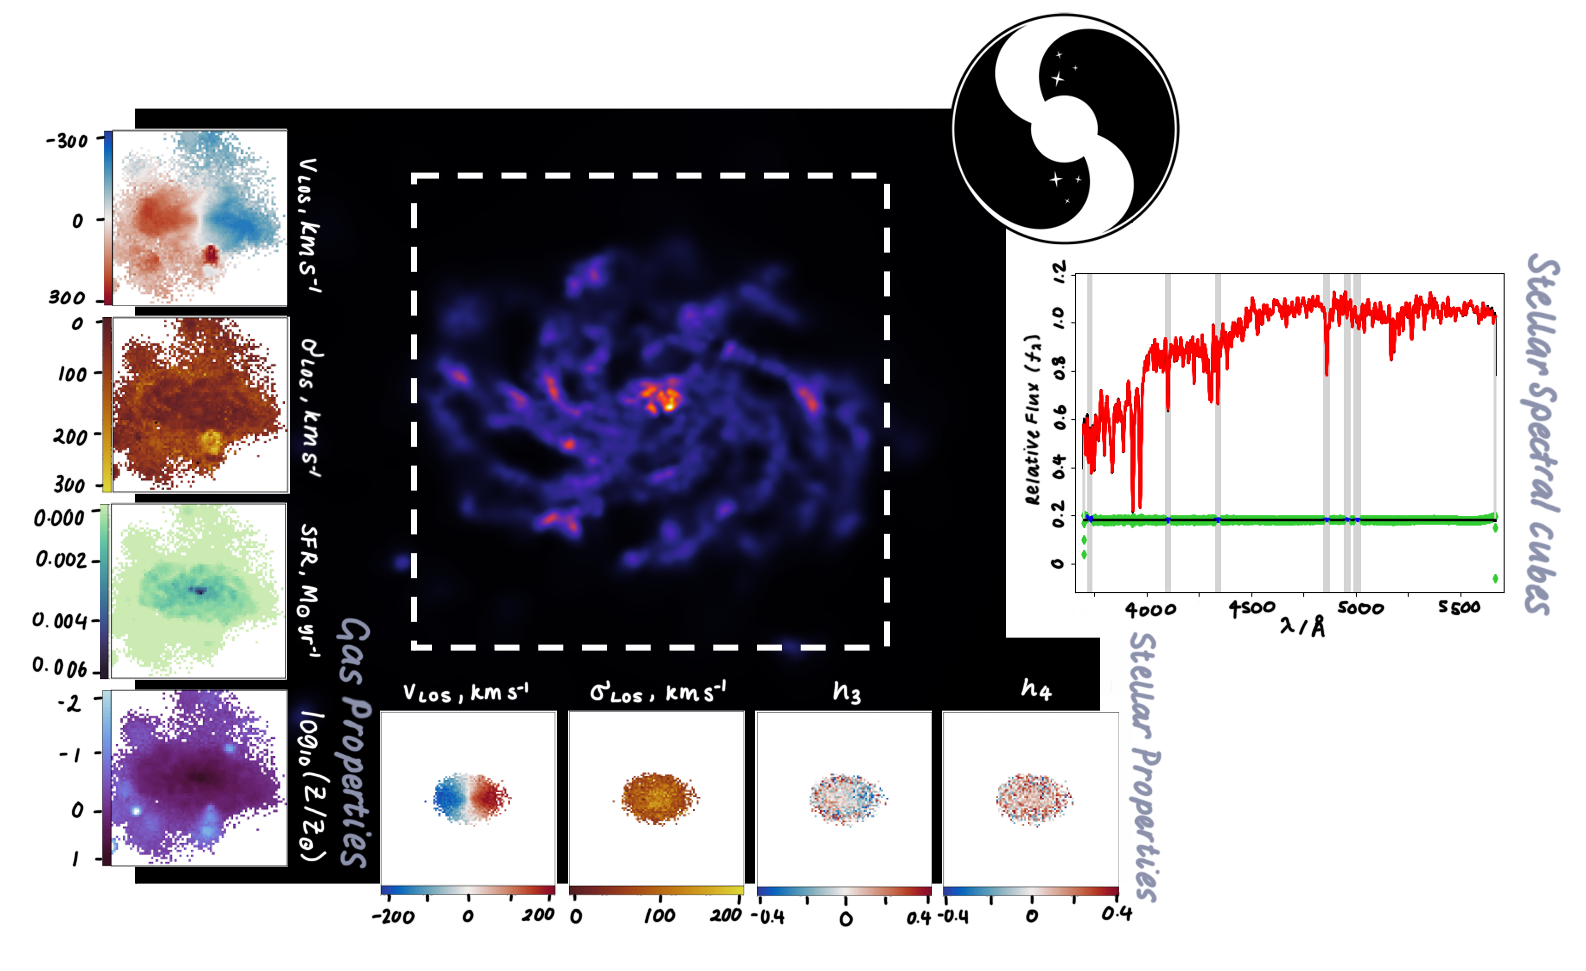
\includegraphics[keepaspectratio, width=14cm]{Figures/simspin_v25.png}
    \caption{Demonstrating the possible outputs of a \simspin{} observation using a MUSE-like telescope on an inclined \eagle{} disk galaxy from the z = 0.271 snapshot of the \texttt{RefL0100N1504} box. To the left, we show the possible outputs from a kinematic data-cube measured for the smoothed gas component. Along the bottom, we show a similar range of possible outputs for a kinematic mode observation of the stellar component. The central image of \eagle{} GalaxyID 16382120 has been made using the code \texttt{SPLASH} \citep{Price2007Splash}. }
    \label{fig:simspin_v2}
\end{figure*}

The key function performed by \simspin{} is the construction of a mock IFS data cube from a galaxy simulation input, as shown in Figure \ref{fig:simspin_v2}. 
In this section, we describe the methodology used for constructing such an observation. 
The process is broken into three steps: (1) preparing the input simulation; (2) preparing the mock observation settings (i.e. telescope and object projection); (3) building the mock data cube. 
This section does not aim to act as documentation for each function, rather to highlight the key methodological principles incorporated at each step. 
For specific documentation and examples, we refer the reader to the live and continuously-updated documentation website \url{https://kateharborne.github.io/SimSpin/}.

The aim is for this code to be agnostic to the type of simulation supplied: smoothed-particle hydrodynamics, adaptive mesh refinement, or $N$-body. 
In all cases, you should receive a consistent and comparable output cube with metadata such that the whole product can be reconstructed with the information contained within the file itself and the input simulation.

\subsection{Creating an input file} \label{sec:make_simspin_file}

We begin with a function, \makesimspinfile, whose purpose is to prepare the simulation into a consistent format. 
This first step allows all other processes to occur in the same way for any type of input simulation or requested telescope.
The function accepts an output simulation file (in either HDF5 or \gadget{} Binary format) and returns a binary (\texttt{.RData}) file in a universal format that \simspin{} can process.

\begin{lstlisting}[basicstyle=\fontsize{6}{8}\selectfont\ttfamily]
make_simspin_file(filename, cores = 1,
                  disk_age = 5, 
                  bulge_age = 10,
                  disk_Z = 0.024, 
                  bulge_Z = 0.001,
                  write_to_file = TRUE, 
                  output, overwrite = F,
                  template = "BC03lr", # spectral template choice
                  centre = NA, half_mass = NA, # alignment choice
                  sph_spawn_n = 1)             # smoothing choice
\end{lstlisting}

\begin{figure*}
    \centering
    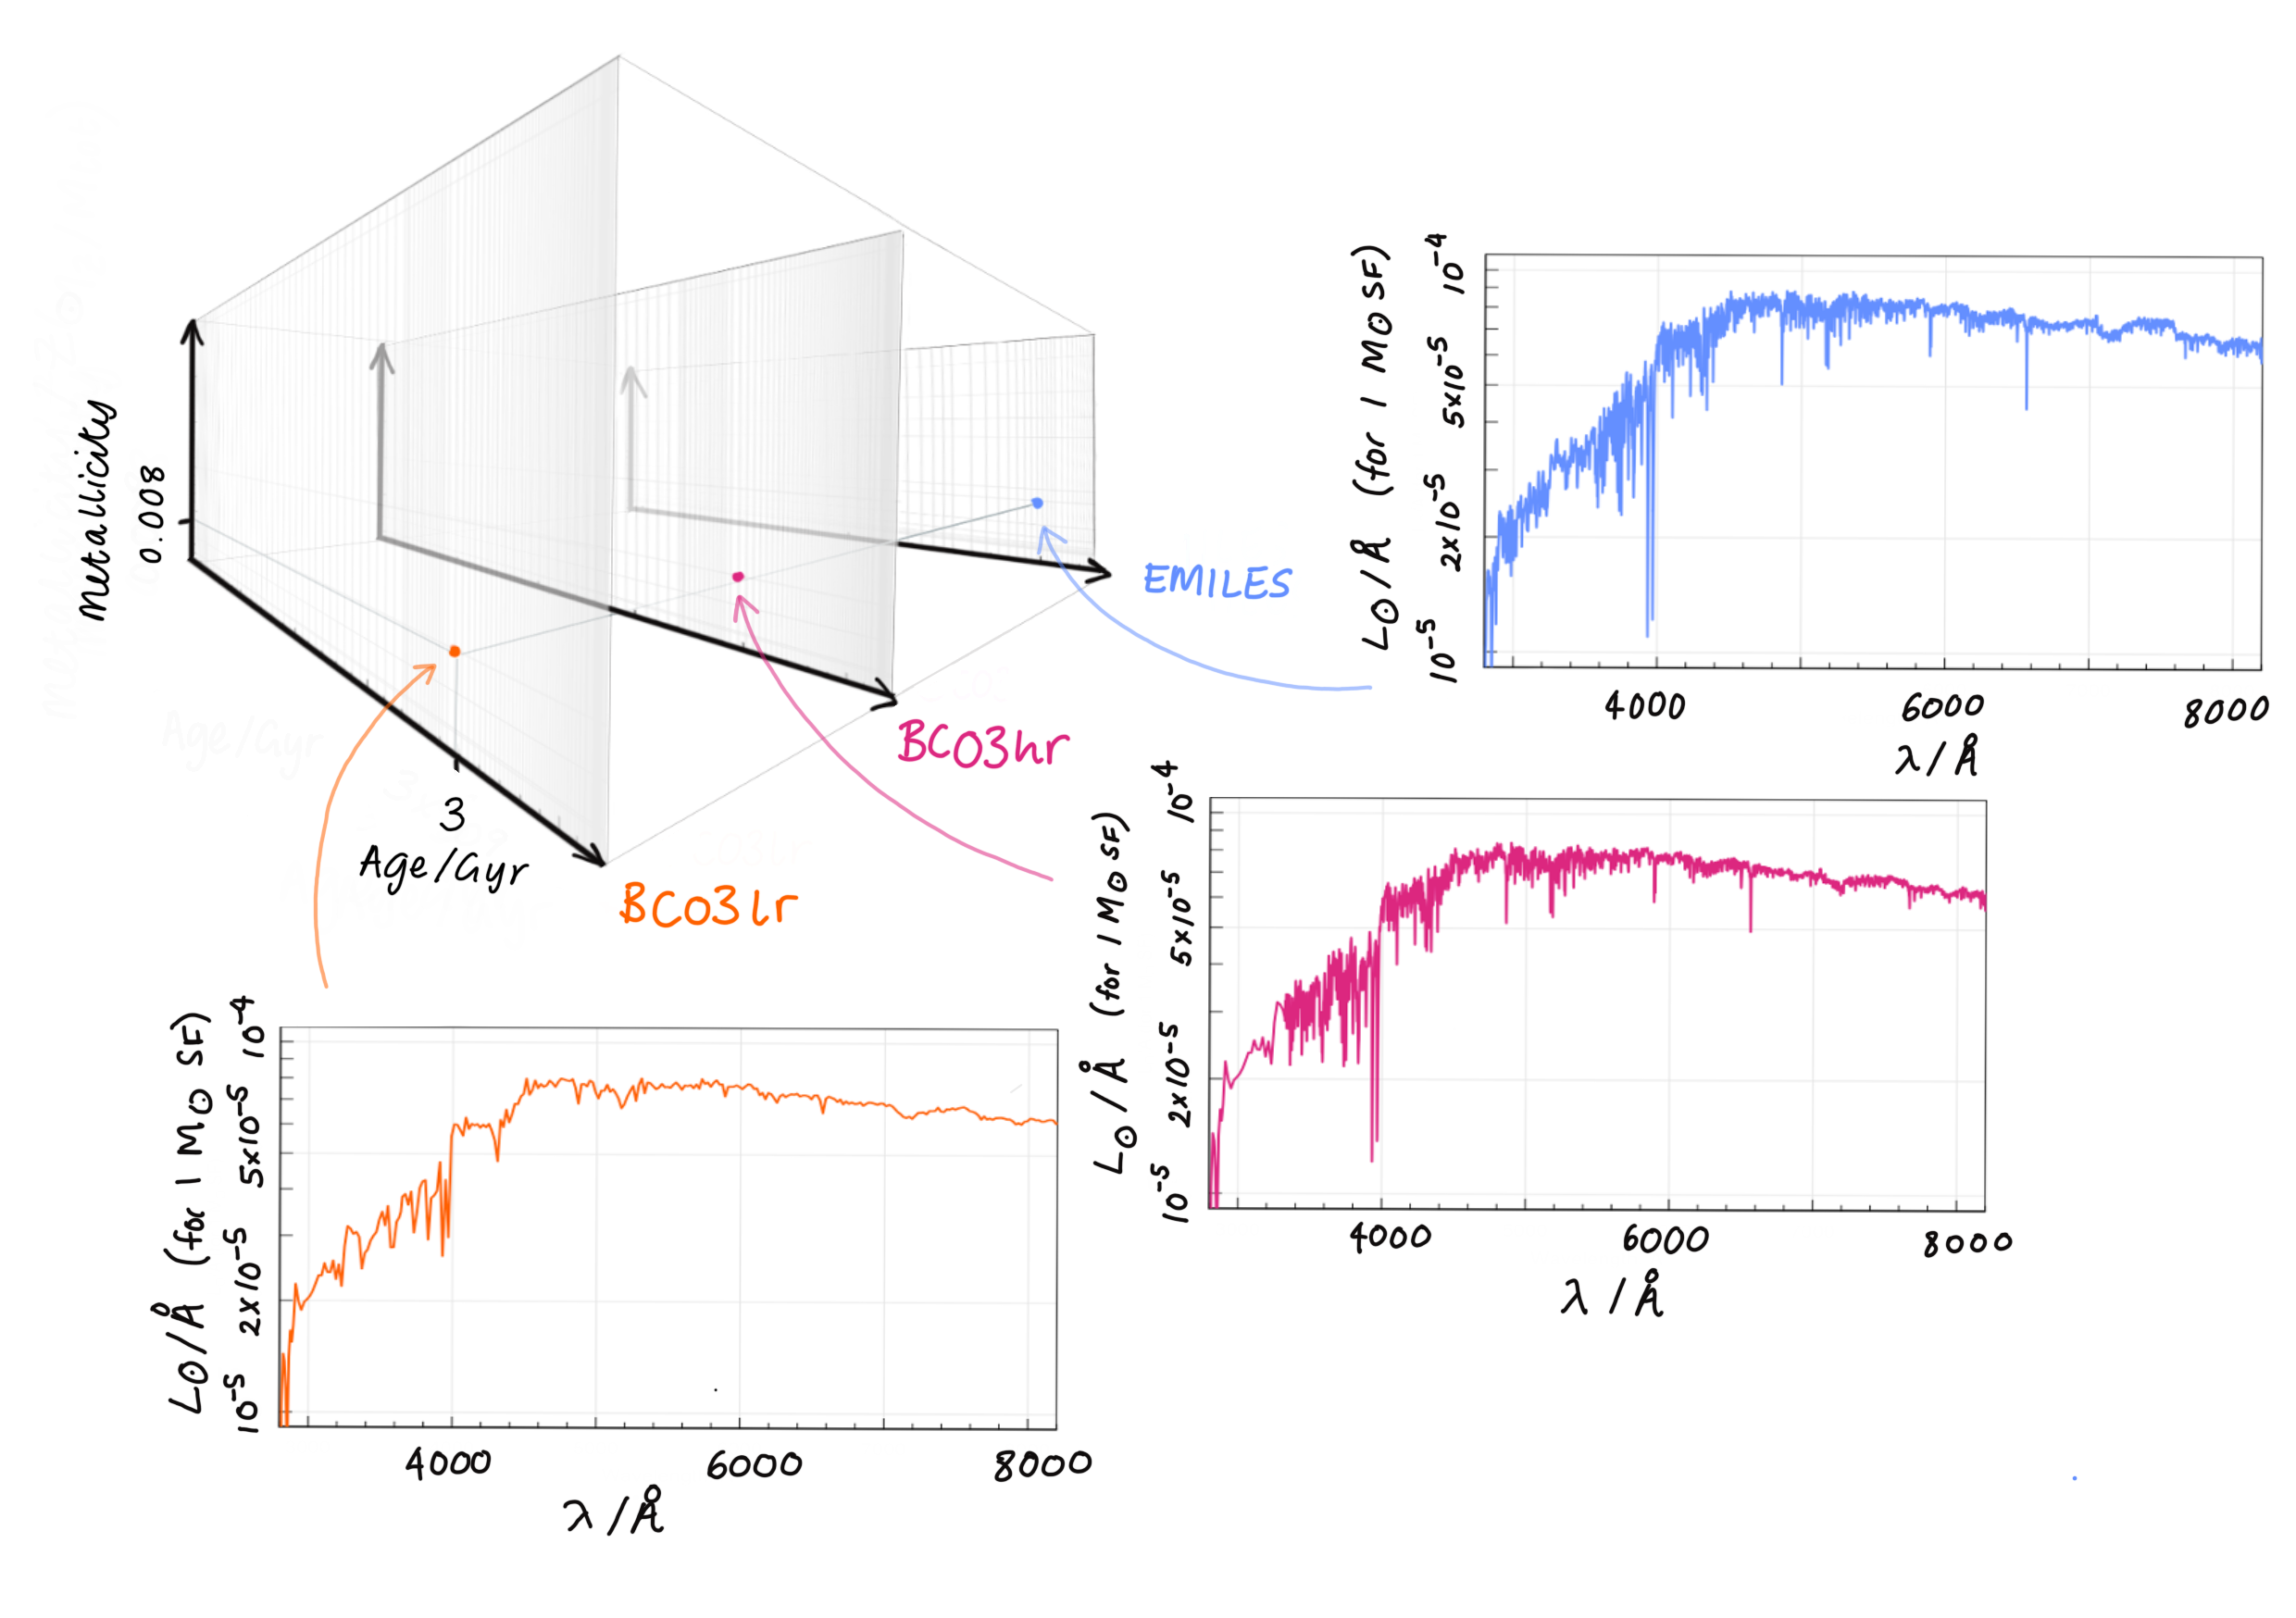
\includegraphics[keepaspectratio, width=14cm]{Figures/simspin_file_method.png}
    \caption{A diagram to explain the role of simple stellar population (SSP) template selection when preparing a SimSpin file. Given a template for a stellar population of a given age and metallicity, we ``tag'' each stellar particle from the simulation with one of the associated spectra. The choice of template library is one for the user dependent on the science you wish to achieve with the mock observations produced, and is obviously dependent on the underlying resolution of both the templates and the simulation in question.}
    \label{fig:SSP_template_selection}
\end{figure*}

Currently, \simspin{} directly supports simulation inputs cut-out from a range of cosmological models including \eagle{}, \magneticum{} Pathfinder, \horizon{} and \illustristng. 
However, the expected format is fully described within the documentation such that any HDF5 file with the required parameters and units can be read and processed by the code. 
Further details about how to format your simulation data for ingestion into \simspin{} can be found through the documentation website\footnote{\url{https://kateharborne.github.io/SimSpin/examples/generating_hdf5.html}}.
We summarise the main important features here. 

Each particle within a simulation will have a number of existing tagged properties used to track their progress throughout the simulation. 
In order to make a \simspin{} observation, the key elements we require include positions ($x, y, z$), velocities ($v_z, v_y, v_z$), and masses for the stellar and/or gas components. 
In order to assign spectra to a given ``stellar'' particle, we also require ages, metallicities and the initial mass of that star. 
In the case of hydro-dynamical simulations, these properties will be tracked throughout the evolution of the system and can be used directly from the output.
For N-body models, in which we are just tracing gravitational effects, we can specify the age and metallicity parameters for the bulge and disk components within the \makesimspinfile{} function to define these values arbitrarily. 
A summary of these necessary particle properties will be tabulated and stored as list elements within the \simspin{} file for later data cube processing. 
The stellar and gas particle properties will be split into two separate data tables, in the case that gas is present in the input model. 

This formatting of the \simspin{} input allows the code specific metadata to be summarised in an efficient way. 
In the output of this file, we summarise the properties of the input simulation (e.g. the simulation type and location of the input file from which this product has been made); the parameter choices (e.g. the name and properties of the chosen spectral templates); as well as a record of the code version used to build the file and the date on which it was constructed. 
This aids the user in inspecting the status of a given file in a human-readable way.
It also enables the user to re-create the same file with the same methodology in the future without needing to retain the code used to generate the file. 

Besides the universal formatting procedure and metadata addition, the main justification for creating a `\simspin{}'-formatted input file is to pre-compute the computationally expensive steps - (1) associating a spectrum with each particle, (2) to align the object within the field of view such that our observations are clearly defined and (3) smoothing gas particle or cell properties across their kernel. 
The galaxy within the output file can be observed multiple times once a single \simspin{} file has been constructed. 
However, there are some choices made at this stage that may depend on the type of observations you wish to make, as highlighted in the code snippet above. 
Further information about these choices will be discussed in this section.

\subsubsection{Spectral template choice}

\begin{table*}[!ht]
    \centering
   \begin{tabular}{@{}llllllll@{}}
    \toprule
    Name & Age Steps & Age Range (Gyr) & Z Steps & Z Range (Z$_{\odot}$) & $\lambda$ Steps (\AA) & $\lambda$ Range (\AA) & LSF FWHM (\AA) \\ \midrule
    `\texttt{BC03lr}' & 221 & 0 - 20 & 6 & 0.0001 - 0.05 & 1221 & 91 - 1.6$\times 10^{6}$ & 3 \\
    `\texttt{BC03hr}' & 221 & 0 - 20 & 6 & 0.0001 - 0.05 & 6990 & 91 - 1.6$\times 10^{6}$ & 3 \\
    `\texttt{EMILES}' & 53 & 0.03 - 14 & 12 & 0.0001 - 0.04 & 53689 & 1680.2 - 49999.4 & 2.51 \\ \bottomrule
    \end{tabular} 
    \caption{Demonstrating the resolution properties of the variety of spectral templates available in \simspin. It is useful to be aware that the resolution of mock data is built upon templates with finite resolution themselves.}
    \label{tab:templates}
\end{table*}

There are currently three options to choose from for spectral templates used to associate spectra with individual particles, which are listed in Table \ref{tab:templates}. 
We give this selection of options as a user may wish to focus on different science question with one set of templates better suited than the other, e.g. for observations with high spectral resolution instruments (such as MUSE), the high resolution template options will be necessary, but these may be avoided in other cases due to the increased memory requirements and computation. 
This suite of templates is also a reflection of those commonly used within the literature for exploring galaxy kinematics. 

%\br{We have ensured that all template spectra available are within the SAFE range of use as specified by ...} 

When selected, the spectral templates within the chosen library are used to tag each stellar particle with an associated spectrum.
We visually demonstrate this particle tagging step in Figure \ref{fig:SSP_template_selection} for some arbitrary stellar particle with age of 3 Gyr and metallicity of 0.008.
Here, the requirement to select the correct template for the science in question is made clear. 
While the EMILES templates are obviously higher spectral resolution ($\Delta \lambda = 0.9$\AA{} with $\sigma_{\text{LSF}} = 2.51$\AA{} in comparison to $\Delta \lambda = 1-50$\AA{} with $\sigma_{\text{LSF}} = 3$\AA{} for the BC03 templates), the grid of possible age and metallicity combinations is more sparse (with 636 combinations in comparison to the 1326 available for the BC03 templates). 

To aid memory load, we further choose to group particles into bins of age and metallicity in order to remove the requirement to save a single spectrum for every particle in a given simulation. 
We justify this by considering the match up between the possible age and metallicity grid for each set of templates and the intrinsic resolution limitations within the simulations themselves.
Taking the range of ages and Z for each simulation, we grid these parameters into bins equally distributed between the minimum and maximum in logarithmic space with widths of \texttt{log10(0.02)} in age and \texttt{log10(0.10)} in metallicity. 
We demonstrate the effect of this binning using an example galaxy from the \eagle{} simulation as shown in Figure \ref{fig:age_metal_bins}. 
Currently, the size of these bins are fixed within the code, but feasibly could be made adjustable to account for ranges in precision between simulations and additional template libraries. 

\begin{figure}
    \centering
    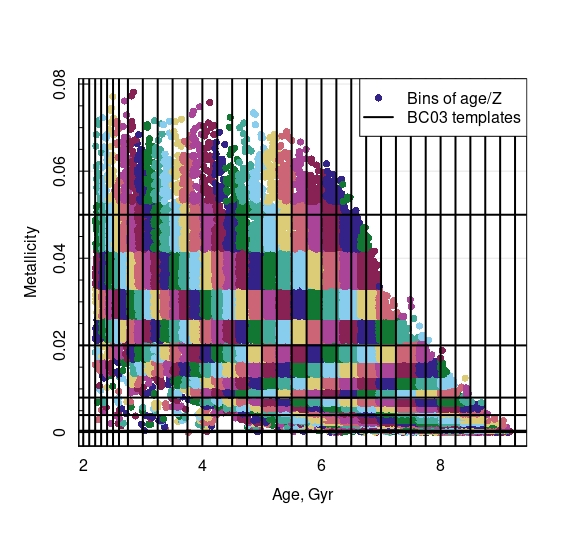
\includegraphics[keepaspectratio, width=7cm]{Figures/age_z_gridding_procedure.jpeg}
    \caption{Demonstrating the gridding of stellar ages and metallicities within the example \eagle{} galaxy (ID 16382120) relative to the higher age/Z resolution GalexEV templates. A single template spectrum is associated with the intersection of each black line. The points show the intrinsic age/Z of each particle. Each coloured cluster of points is assigned an age and Z at the centre of the cluster and all points in each cluster will be associated with a single spectrum. That assigned spectrum will be a weighted combination of the four nearest template spectra to that cluster.}
    \label{fig:age_metal_bins}
\end{figure}

Individual age-metallicity bins for each group of particles do not necessarily line up with the grid of available templates within the chosen library. 
The assigned spectrum for a given age-metallicity bin are computed as a weighted interpolation of the four nearest template spectra. 
These are then stored in a list element of the file, with references to each ``spectrum'' row stored in the stellar particle data table.

\subsubsection{Alignment choice}
By default, the galaxy is aligned such that the semi-major axis of an ellipsoid is oriented with the $x$-axis of the reference frame, and the minor axis of the ellipsoid is oriented with the $z$-axis. 
This provides consistency for multiple observations made at a variety of inclination angles. 
However, in the case that a full cluster, galaxy group, or a particularly `clumpy' galaxy with lots of substructure is requested for observation, this alignment will be arbitrary. 

Hence, \simspin{} gives the user the option to define a single location around which to centre the system (\texttt{centre}) and define a half-mass value at which the shape of the galaxy will be measured (\texttt{half\_mass}). 
If unspecified, the code will evaluate the alignment about the median stellar particle position with an iteratively fit ellipsoid that contains half the total stellar mass in the input file. 

This alignment is done using the method described in the work of \citealt{Bassett2019GalaxyShapes},  \citep[which in turn is based on the work from][]{Li2018TheShapesIllustris, Allgood2006ShapeDarkMatterHaloes}. 
We first assume that the initial distribution of stellar particles is an ellipsoid with axis ratios $p = q$ (i.e. a sphere, where $p = b/a$ and $q = c/a$, with $a, b$ and $c$ representing the axes lengths in decreasing size such that $a > b > c$ and $p > q$, by necessity).  
This ellipsoid is grown from the median position of all stellar particles within the file (or from the position specified by \texttt{centre}) until it contains half the total stellar mass within the file (or the threshold mass described by the specified \texttt{half\_mass} parameter input). 
Once this limit is reached, we use the stellar particles within the region to measure the reduced inertia tensor. 

The reduced inertia tensor, $I$, is computed:
\begin{equation}
    I_{i,j} = \sum_n{\frac{M_n x_{i,n} x_{j,n}}{r^2_n}},
\end{equation}
where we perform this sum for $n$ stellar particles within the ellipsoid with given positions, $x_n$, weighted by individual stellar particle masses, $M_n$, which may vary within the simulation and $r_n$, the 3D radius of that particle from the centre as described by,  
\begin{equation}
r_n = \sqrt{x_n^2 + y_n^2 / p^2 + z_n^2 / q^2}.    
\end{equation}

The eigenvalues and eigenvectors of this tensor, $I_{ij}$ give the orientation and distribution of matter within the ellipsoid. 
Specifically, $p$ and $q$ are given by the square-root of the ratios between the intermediate and largest eigenvalues ($b$ and $a$) and the smallest and largest eigenvalues ($c$ and $a$) respectively. 

The ellipsoid is then deformed to match the distribution of stellar particles.
The whole system is reoriented such that the major axis of the distribution identified is now aligned with the major axis of the ellipsoid. 
We then begin the procedure again, this time growing an ellipsoid with new $a, b,$ and $c$ reflecting the matter distribution of the stellar particles contained. 
This is repeated until the axis ratios $p$ and $q$ stabilise over ten iterations. 

All particles within the input simulation file are aligned with the major axis, $a$, along the $x$-axis of the volume and the minor axis, $c$, aligned with the $z$-axis using this method. 
In the majority of cases, we find that this is suitable for finding the underlying shape of the galaxy in question and aligning the object suitably within the frame. 
In a data set of 1835 galaxies taken from the IllustrisTNG50-1 simulation, a comparison between the alignment found by the \texttt{mgefit.find\_galaxy} function \citep{Cappellari2002Efficientgalaxies} and \simspin{} revealed that 92.3\% (1693/1835) of the alignments agreed within ten degrees. 
Caution is advised when making mock observations of ellipticals or galaxies undergoing merging, as a visual analysis of the farthest outliers found most fell under these categories.

This allows us to correctly re-orient the galaxy to the user specified inclination and twist projection at the stage of building the mock data cubes. 
In cases where the semi-major axis is not well defined, this can be adjusted for purpose with some experimentation of the alignment parameters, \texttt{centre} and \texttt{half\_mass}.


\subsubsection{Smoothing choice}
In the case of galaxies extracted from hydrodynamical simulations, a population of particles or cells trace the underlying distribution of a fluid (such as the gas in a galaxy). 
Properties of the fluid are computed across a volume, described by the smoothing `kernel' or cell size, centred at the given location. 
In order to ensure that we reproduce this smoothing in our data cubes and recover the underlying fluid properties appropriately within our images, we use an over-sampling method to visualise this kernel volume.

This means that, when we generate a mock observation of the gas component, we must project particles with adaptive sizes onto a fixed grid of pixels. 
As discussed in \citealt{Borrow2021ProjectingEnvironments}, there are many methods of doing this.
However, many of the simple methods result in inaccuracies and artifacts due to the projection of spherical kernels onto a rectangular grid.

The basic SPH kernel projection method is outlined in \citealt{Borrow2021ProjectingEnvironments} (a flavour of which is used in \citealt{Dolag2005ThePlanck}).
We have taken the sub-sampling regime described in these papers and redesigned them for use in \simspin{}. 
Particles are treated as Monte Carlo tracers of the field. 
The basic features of this algorithm are stated below:

\begin{enumerate}
    \item Each SPH particle read in contains information about its ``smoothing length'', $h$, across which hydrodynamical equations have been computed for the fluid represented at that particle position. In the case of AMR codes, the equivalent information about the ``cell size'' is used. 
    \item We randomly sample \texttt{sph\_spawn\_n} tracer particles within a sphere centred on the true SPH particle position. 
    \item Each tracer particle is associated with a numerical weight as described by the relevant SPH kernel. 
    All weights for an individual SPH particle will sum to one in order to conserve mass within the system.
    \item These new tracer particles replace the original SPH particle. 
    They gain all the properties of the original particle, but a weighted fraction of the total mass according to the weight assigned using the kernel. 
\end{enumerate}

This results in a new table of particle properties. 
The new table will contain \code{`sph\_spawn\_n'} times as many rows as the original component of SPH particles. 
However, once this table have been computed, the processing of these observations with \builddatacube{} will be very quick due to the $\mathcal{O}(n)$ computation used to grid particles into pixels. 
For this reason, we perform the smoothing at the point of making the \simspin{} input file, rather than at the \builddatacube{} step. 

When using this option, we attempt to ensure that the projection kernel corresponds to the kernel used for the SPH calculations within the simulation. 
For supported hydrodynamic simulations, we provide a smoothing kernel to best match the one used in the original model.
These are selected automatically based on the metadata contained within the input file. 

Most SPH simulations use a flavour of the Wendland kernel outlined in \citealt{Wendland1995PiecewiseDegree}. 
The $C^{2}$ Wendland kernel, used in \eagle{} \citep{Schaller2015TheScheme}, is a spherically symmetric kernel, $W(r,h)$, which has the form: 
\begin{equation}
    W(r,h) =
    \begin{cases}
        \frac{21}{2 \pi}(1 - r/h)^4 (4r/h + 1),& \text{if }\ 0 \leq r/h < 1\\
        0,                                     & \text{if }\ r/h \geq 1
    \end{cases}
\end{equation}
Here, $r$ denotes the distance from the particle to another position at which the weight is calculated and $h$ denotes the smoothing length of a particle. 
For each simulation, this smoothing length, $h$, is a value given by requiring that the weighted number of nearest neighbouring particles, $N_{neigh}$, is a pre-defined constant:
\begin{equation}
    N_{neigh} = \frac{4 \pi h_i^3}{3} \sum_j W\left(|x_i - x_j|, h_i \right).
\end{equation}
For the \eagle{} simulation, $N_{neigh} = 48$, but this will vary for each SPH simulation.
This smoothing length is computed for each particle throughout the simulation, as this value will obviously be dependent on the the local number density of particles.
The smoothing length, $h$, is commonly stored as a parameter within the output files. 
We can use this parameter to then determine the radius across which each individual gas particle should be over-sampled.   

The $C^{6}$ Wendland kernel used in \magneticum{} \citep{Teklu2015ConnectingMorphology} has the form:
\begin{equation}
    W(r,h) =
    \begin{cases}
        \frac{1365}{64 \pi}(1 - r/h)^8 \times \\ \hspace{3ex} (1 + 8 r/h  + 25 (r/h)^2 + 32 (r/h)^3),& \text{if }\ 0 \leq r/h < 1\\
        0,                                     & \text{if }\ r/h \geq 1
    \end{cases}
\end{equation}
In \magneticum{,} the smoothing lengths have been computed with $N_{neigh}=64$ \citep{Beck2016Ansimulations}, but again, the raw $h$ for each particle is given in the output for this simulation. 
When 

Finally, in the case of \gadget{} SPH simulations, and for visualisation of AMR/cell model implementations, we use the M4 cubic spline kernel to smooth gas distributions across our image grid.
In particular, for mesh-based codes, we do not have a smoothing length for a given cell. 
As an approximation, we use the quoted cell density and mass to compute an ``effective'' smoothing length at a position at the centre of the cell (at the position where cell properties are given).
\begin{equation}
    h_i = 2 \frac{3}{4 \pi} \left( M_i / \rho_i\right)^{1/3}
\end{equation}
where the effective smoothing length, $h$, for a given cell, $i$, is the mass within that cell, $M_i$, divided by the density of the cell, $rho_i$. 
A spherical distribution is assumed so that the system can be observed fairly from any angle without observing discontinuities at low density locations.  

We then use a simplest appropriate kernel, the M4 cubic spline kernel, as an approximation of the behaviour of the gas within a given cell:
\begin{equation}
    W(r,h) =
    \begin{cases}
        \frac{1}{4 \pi} \left((2 - r/h)^3 - (1 - r/h)^3\right) ,& \text{if }\ 0 \leq r/h < 1\\
        0,                                     & \text{if }\ r/h \geq 1
    \end{cases}
\end{equation}

This approximation is used for visualisation of \horizon{} and \illustristng{} simulations. 

\vspace{0.5cm}

\noindent Once this file is created for one simulated object, it can be used many times for observations. 
This file contains all of the multi-dimensional information from the simulation file, with an additional set of tagged properties for \simspin{} to construct each cube. 


\subsection{Initialising the telescope and observing strategy}

\simspin{} acts as a virtual telescope wrapper. 
You can choose to observe your galaxy model in a variety of different ways with any integral field unit (IFU) instrument. 
This requires you to set two distinct groups of properties - the properties of the instrument used to take the observation i.e. the \telescope{}, and the properties of the object under scrutiny i.e. the \observingstrategy{}. 

The properties are split in this way to enable a suite of observations to be generated in a straightforward manner. 
It is common that an observer will wish to observe a suite of galaxies using the same telescope, but may want to iterate over a number of projected inclinations, distances or seeing conditions. 
Hence, we have split the description classes for the observing telescope and observed object properties into two. 
We describe the mathematics behind the functions in the sections below, but direct the reader to the specific documentation pages\footnote{\url{https://kateharborne.github.io/SimSpin/docs/documentation}} for up-to-date, detailed examples of running each function.

\subsubsection{Telescope choice}

\begin{lstlisting}[basicstyle=\fontsize{6}{8}\selectfont\ttfamily]
telescope(type="IFU",  
          fov=15,                             
          aperture_shape="circular", 
          wave_range=c(3700,5700),   
          wave_centre,              
          wave_res=1.04,    
          spatial_res=0.5, 
          filter="g",      # luminosities output in this band  
          lsf_fwhm=2.65,
          signal_to_noise = NA) # target signal-to-noise ratio

\end{lstlisting}

\simspin{} has a number of predefined IFU telescopes, for which the required field-of-view, spectral and spatial resolutions have been taken from the available literature. 
In Table \ref{tab:telescope_options}, we describe the values associated with these defaults and their appropriate references. 

For a number of these choices, there are further selections that can be made. 
For example, the ``MaNGA'' telescope has a variable field-of-view size that the user can select.
If a specific telescope ``type'' is not covered by the available options, the parameters can be fully specified by using the \texttt{type = "IFU"}. 
This requires the user to describe the remaining parameter options of the telescope, including the field-of-view size in arcseconds, the shape of the aperture, the wavelength range and central peak wavelength in \AA, the wavelength resolution in \AA, the spatial resolution in arcseconds, and the associated line-spread function (LSF) of the instrument in \AA.
Two parameters can be further altered by the user when using the predefine telescope types: the filter, and the minimum level of signal-to-noise. 

\begin{table*}[ht!]
\caption{A list of predefined parameters for each \telescope{} ``type'' available in \ssversion. A number of these parameters are variables that the user can further specify, which have been emphasised in bold below.}
\label{tab:telescope_options}
\begin{tabular}{lllllll}
\hline
\textbf{Telescope parameter} & \textbf{Units} & \textit{SAMI} & \textit{MaNGA} & \textit{CALIFA} & \textit{MUSE} & \textit{Hector} \\
 &  & \citep{Croom2012SAMIOverview} & \citep{Bundy2015OverviewObservatory} &  &  &  \\ \hline
\texttt{fov} & arcsec & 15 & \textbf{n = 12, 17, 22, 27 or 32} & 74 & \textbf{n} \textless \textbf{60} & 30 \\
\texttt{aperture\_shape} &  & "circular" & "hexagonal" & "hexagonal" & "square" & "hexagonal" \\
\texttt{wave\_range} & \AA{} & 3750 - 5750 & 3600 - 6350 & 3700 – 4750 & 4700.15 - 9351.4 & 3720 - 5910 \\
\texttt{wave\_centre} & \AA{} & 4800 & 4700 & 4225 & 6975 & 4815 \\
\texttt{wave\_res} & \AA{} & 1.04 & 1.04 & 2.7 & 1.25 & 1.60 \\
\texttt{spatial\_res} & arcsec/pixel & 0.5 & 0.5 & 1 & \textbf{0.2 (WFM) or 0.025 (NFM)} & 0.2 \\
\texttt{lsf\_fwhm} & \AA{} & 2.65 & 2.85 & 2.7 & 2.51 & 1.3 \\ \hline
\end{tabular}
\end{table*}

The available filters in \simspin{} \ssversion{} include the SDSS $u$, $g$, $r$, $i$ and $z$ filters \citep{Doi2010PhotometricImager}. 
Details of these filters, including the range across which they act, are listed in Table \ref{tab:available_filters}.
Each of these data tables are stored as an \texttt{rda} file optimally compressed using \texttt{xz} compression such that they are lazy loaded with the package. 
The associated documentation gives the location from which these data have been collected. 
As with the predefined telescope types, the list of available filters may grow in time.
Any updates will be listed on the live documentation website. 
These filters are then ready to be used in the \builddatacube{} function.

\begin{table}[ht!]
\caption{The relative response of the available filters across the relevant wavelength range in Angstroms.}
\label{tab:available_filters}
\begin{tabular}{@{}lll@{}}
\toprule
\textbf{Filter Name} & \textbf{Wavelength Range, \AA}  \\ \midrule
\texttt{filt\_u\_SDSS} & 2980 - 4130 \\
\texttt{filt\_g\_SDSS} & 3630 - 5830 \\
\texttt{filt\_r\_SDSS} & 5380 - 7230 \\
\texttt{filt\_i\_SDSS} & 6430 - 8630 \\
\texttt{filt\_z\_SDSS} & 7730 - 11230 \\ \bottomrule
\end{tabular}
\end{table}

The signal-to-noise specified will be implemented in spectral and \rb{kinematic data cubes.} Following the mathematical implementation of noise to cubes given in \citealt{Nanni2022iMaNGAcubes}, we similarly scale the level of Gaussian perturbation added to each spectrum based on the total flux measured at each pixel:
\begin{equation}
    \frac{dF_i}{F_i} = \frac{\sqrt{F_{\text{max}}}}{S/N \times \sqrt{F_i}},
\end{equation}
where $dF/F$ is the maximum fractional perturbation of flux within a given spaxel $i$, $S/N$ is the requested parameter given in the \telescope{} function, and $F_{\text{max}}$ is the maximum flux from the observation. 
At each spaxel, we draw a random number from a Gaussian distribution, scaled by this $dF/F$, and add this perturbation as a function of wavelength to each spectrum. 
For kinematic cubes, this perturbation is applied to the observed fluxes alone. 

With the \telescope{} elements defined, parameters can be precomputed. 
The number of spatial pixels, \texttt{sbin}, required to fill the diameter of the field-of-view (FOV) is computed and stored for gridding purposes. 
When combined with the coordinate information for a simulation at the \builddatacube{} stage, we can use the following simple equation to label each particle with a corresponding pixel in the FOV of the telescope. 
We bin the particle data along the $x$- and $y$-axes respectively ($x_{\text{bin}}$ and $y_{\text{bin}}$) labelling each bin with an integer value from 1 to \textt{sbin} and then combine these using,
\begin{equation}
    \texttt{pixel\_pos} = x_{\text{bin}} + (\texttt{sbin} \times y_{\text{bin}}) - \texttt{sbin},
\end{equation}
such that every pixel within the FOV has a unique identifier which can be associated with each particle within the model at the \builddatacube{} stage.

Checks are also performed at this stage such that a user does not waste the time loading in a large simulation file only to have the code fall over because of a filter mismatch. 
We ensure that the requested filter will overlap with the telescope wavelength range coverage and the centre of this wavelength range, if not provided, is computed as the centre of the given range. 
A further check is made for the variable parameters such as \textsc{MaNGA} field-of-view, that the requested value is one of the available bundle sizes (i.e. 12, 17, 22, 27 or 32). 
If not, the closest value larger than the requested parameter will be taken by default and a warning will be issued.
Similarly, if a user asks for a MUSE cube with greater than 60'' field-of-view, the value will be rounded down. 
Users will also be able to specify wide-field mode (WFM) in which spaxels are 0.2'' or near-field mode (NFM) where spaxels are 0.025'' for MUSE. 
If another value is suggested, the function will default to WFM (as this is the most computationally efficient) and issue a warning to the user that this has occurred. 

Further default telescope types will be added in the future to keep up with ongoing developments.
The live documentation will reflect any changes made.

\subsubsection{Observation strategy choice} \label{sec:observation}
\begin{lstlisting}[basicstyle=\fontsize{6}{8}\selectfont\ttfamily]
observing_strategy(dist_z       = 0.05,   # projected distance
                   inc_deg      = 70,     # projected angle
                   twist_deg    = 0,      
                   pointing_kpc = c(0,0), # telescope centre 
                   blur         = T,      # seeing conditions
                   fwhm         = 1,
                   psf          = "Gaussian")      
\end{lstlisting}

Another necessary ingredient for specifying a mock observation is the description of the conditions in which the model galaxy is observed.
How far away is the object? 
How is it projected on the sky? 
How severe are the seeing conditions?
These properties are specified using the \observingstrategy{} function. 

It is expected that an individual may wish to observe the same galaxy at a range of distances, inclinations, and seeing conditions, while the overall properties of the \telescope{} are more likely to remain fixed.\footnote{It is also possible to iterate over a range of these parameters to produce a series of observations using \texttt{lapply} within R, an example of which can be found at \url{https://kateharborne.github.io/SimSpin/docs/observing_strategy.html}.}

To describe the distance to the observed galaxy model, the user may specify a redshift distance (\texttt{dist\_z}), a physical luminosity distance in Mpc (\texttt{dist\_Mpc}) or an angular scale distance in kpc per arcsecond (\texttt{dist\_kpc\_per\_arcsec}).
When any one of these parameters are specified, the other two are calculated through the S4 \texttt{Distance} class using the following methods \citep{Hogg1999DistanceCosmology} implemented in the \small{R} package \texttt{celestial}\footnote{\url{https://github.com/asgr/celestial}}:
\begin{align}
    \texttt{dist\_z} &= z, \\
    \texttt{dist\_Mpc} &= (1 + z) \; D_{M}(z), \\
    \texttt{dist\_kpc\_per\_arcsec} &= D_{M}(z) / (1 + z), 
\end{align}
where:
\begin{align}
    D_{M}(z)&= D_{H} \frac{1}{\sqrt{|\Omega_k|}} \; \text{sin}\left[D_C \int^z_0 \frac{dz}{E(z)}\right] \; \text{if } \; \Omega_{k} < 0, \\
    E(z) &= \sqrt{\Omega_{M} (1 + z)^3 + \Omega_k (1+z)^2 + \Omega_\Lambda}. 
\end{align}

Given one of the distance measures, the inverse are computed and all measurements returned. 

The inclination and twist parameters define how the model is projected onto the sky. 
Following the \makesimspinfile{} function, the system is aligned such that the major axis of the ellipsoid ($a$) is aligned with the $x$-axis, while the minor axis ($c$) is aligned with the $z$-axis. 
With this knowledge, we can then use basic trigonometry to incline the ellipsoid to a requested inclination and twist.

The inclination of the object describes the level of rotation about the $x$-axis. 
We use the definition that \texttt{inc\_deg} $= 0$ is a face on system, while \texttt{inc\_deg} $= 90$ is edge-on. 
The following mathematics then gives us the coordinates at which the particles would be observed in the $y$- and $z$-axis frames. 
\begin{align} \label{eqn:inc1}
    y^{obs}_i &= - y_i \text{sin}(\frac{\pi}{180} \texttt{inc\_deg}) + z_i  \text{cos}(\frac{\pi}{180} \texttt{inc\_deg}), \\
    z^{obs}_i &= y_i \text{cos}(\frac{\pi}{180} \texttt{inc\_deg}) + z_i \text{sin}(\frac{\pi}{180} \texttt{inc\_deg}), \label{eqn:inc2}
\end{align}
where the $y^{obs}_i$ and $z^{obs}_i$ denote the observed $y$ and $z$ coordinates of particle $i$ in the rotated frame, and $y_i$ and $z_i$ are the $y$ and $z$ coordinates in the original, fixed ellipsoid frame. 
The same projections are used for the velocities observed along the rotated $y$- and $z$-axis.

Similarly, the twist of the object is described as the rotation about the $z$-axis of the ellipsoid. 
Here, \texttt{twist\_deg} $= 0$ is an object viewed with the major axis, $a$, parallel to the $x-$axis of the projection, while \texttt{twist\_deg} $= 90$ would be the ellipsoid viewed from the side, such that $a$ is now aligned with the $y$ axis instead. 
This is computed using similar trigonometric projections as above, 
\begin{align} \label{eqn:twist1}
    x^{obs}_i &= x_i \text{cos}(\frac{\pi}{180} \texttt{twist\_deg}) - y_i \text{sin} (\frac{\pi}{180} \texttt{twist\_deg}), \\
    y^{obs}_i &= x_i \text{sin} (\frac{\pi}{180} \texttt{twist\_deg}) + y_i \text(cos) (\frac{\pi}{180} \texttt{twist\_deg}). \label{eqn:twist2}
\end{align}
where, as above, the $x^{obs}_i$ denotes the observed $x$  coordinates of particle $i$ in the rotated frame, and $x_i$ is the $x$ coordinate in the original, fixed ellipsoid frame. 
The same equations are used to project the particle velocities.

These projections are performed in the order discussed, i.e. the galaxy ellipsoid is inclined on the sky using Equations \ref{eqn:inc1}-\ref{eqn:inc2} and then twisted using Equations \ref{eqn:twist1}-\ref{eqn:twist2}, such that the object can be observed from any angle across the surface of a sphere. 
This is important for exploring the effects of inclination and projection on the recovery of galaxy kinematics.

The final specification of \observingstrategy{} describes the level of atmospheric seeing via the parameters \texttt{psf} and \texttt{fwhm}, describing the shape and full-width half-maximum size of the point-spread function (PSF) smoothing kernel respectively. 
We compute and store the kernel shape here, for each image plane of the observed cube to be convolved at a later stage. 

Two options are currently available to the user, where the \texttt{psf} may be described by a ``Gaussian''kernel, or a ``Moffat'' kernel \citep{Moffat1969APhotometry} which has a Normal-like distribution at the centre with more extended wings. 
These are taken from the parameterisation in the \small{R} package \texttt{ProFit} \citep{Robotham2017ProFit:Images}. A Gaussian kernel is parameterised:
\begin{equation}
    I(R) = I_0 \; \text{exp}\left(- \frac{R^2}{2 \sigma^2}\right),
\end{equation}
where,
\begin{equation}
    \sigma = \frac{\texttt{FWHM}}{2 \sqrt{2\text{ln}(2)}}
\end{equation}
and $I_0$ is the peak intensity at the centre and the \texttt{FWHM} is the value specified in the function. A Moffat kernel is parameterised:
\begin{equation}
I(R) = I_0 \left[ 1 + \left(\frac{R}{R_d}\right)^2 \right],
\end{equation}
where,
\begin{equation}
    R_d = \frac{\texttt{FWHM}}{2\sqrt{2^{1/c} - 1}}
\end{equation}
and $c = 5$, in line with the common defaults.
We ensure that the kernel is normalised to 1 such that convolution with the kernel results in suitable flux conservation.
These kernels are then stored for use in the blurring step later on. 

\vspace{0.5cm}

Having specified the nature of the observation, these functions (\telescope{} and \observingstrategy) are combined to summarise the properties of the resulting observation. 
This is stored as metadata in the final data cube produced.
Storing the data in this way ensures that the same file can be produced at a later time using the information stored in the output cube alone. 
With these parameters specified, we can now go about building our mock observation. 

\subsection{Building a data cube}

Once the observing telescope and properties of the underlying galaxy have been specified, we can go about building a mock observation. 
Within \simspin, we present the user with an option at this stage. 
Either, a series of kinematic maps can be generated from the line-of-sight velocity distributions at each spaxel using the 3D velocity information present for stars, gas or just star-forming, cold gas in the simulation; or, you can choose to create a spectral cube using the stellar spectra themselves, shifted in wavelength space to reflect those underlying velocities and projected redshift distance. 
The resulting spectral cube needs to be run through observational software to generate kinematic maps, and as such is useful for exploring the reliability of reduction pipelines.
This choice is specified in the input parameters by the key word \texttt{method}:

\begin{lstlisting}[basicstyle=\fontsize{6}{8}\selectfont\ttfamily]
build_datacube(simspin_file,              
               telescope,           
               observing_strategy,  
               method = "spectral", # "velocity","gas","sf_gas"
               verbose = F, 
               write_fits = F)  
\end{lstlisting}

The behaviour of the code will be different depending on the method chosen, though the outputs of the \texttt{method = ``spectral``} and \texttt{``kinematic``} are equivalent once run through an observational fitting code such as pPXF \citep{Cappellari2004ParametricLikelihood, Cappellari2017ImprovingFunctions}.
We demonstrate this equivalence in the results section. 

Despite the differences in the type of output, the structure and format followed for the two methods is also consistent. 
Whether we are building a kinematic data cube, or a spectral one, the process of re-projecting the model galaxy to a given orientation (using the information provided in the \observingstrategy) and gridding particles into the necessary pixel locations is done in the same way (using the \telescope{} specific information) before splitting off into method specific functions. 

The output of \builddatacube{} will always include five list elements containing (1) the observed data cube, (2) the metadata table recording the details of the observation, (3) the raw particle property images for reference against, (4), the observed kinematic property images and (5) the observed inverse variance cube ($1/noise^2$).
The final two image elements (``raw'' and ``observed'')  will vary in length depending on the type of observation requested. 
These are summarised in each \texttt{method} description below. 

\subsubsection{Spectral data cubes} \label{sec:spectral_cubes}

If \texttt{method = "spectral"}, the \builddatacube{} function will return a data cube containing spatial information along the $x-$ and $y-$axes of the cube, and wavelength information along the $z-$axis.  
As particles have been allocated to individual pixels within the FOV, we can parallelise over each pixel and perform the mathematics at each pixel in turn, as demonstrated in Figure \ref{fig:spectral_methodology}.

\begin{figure*}
    \centering
    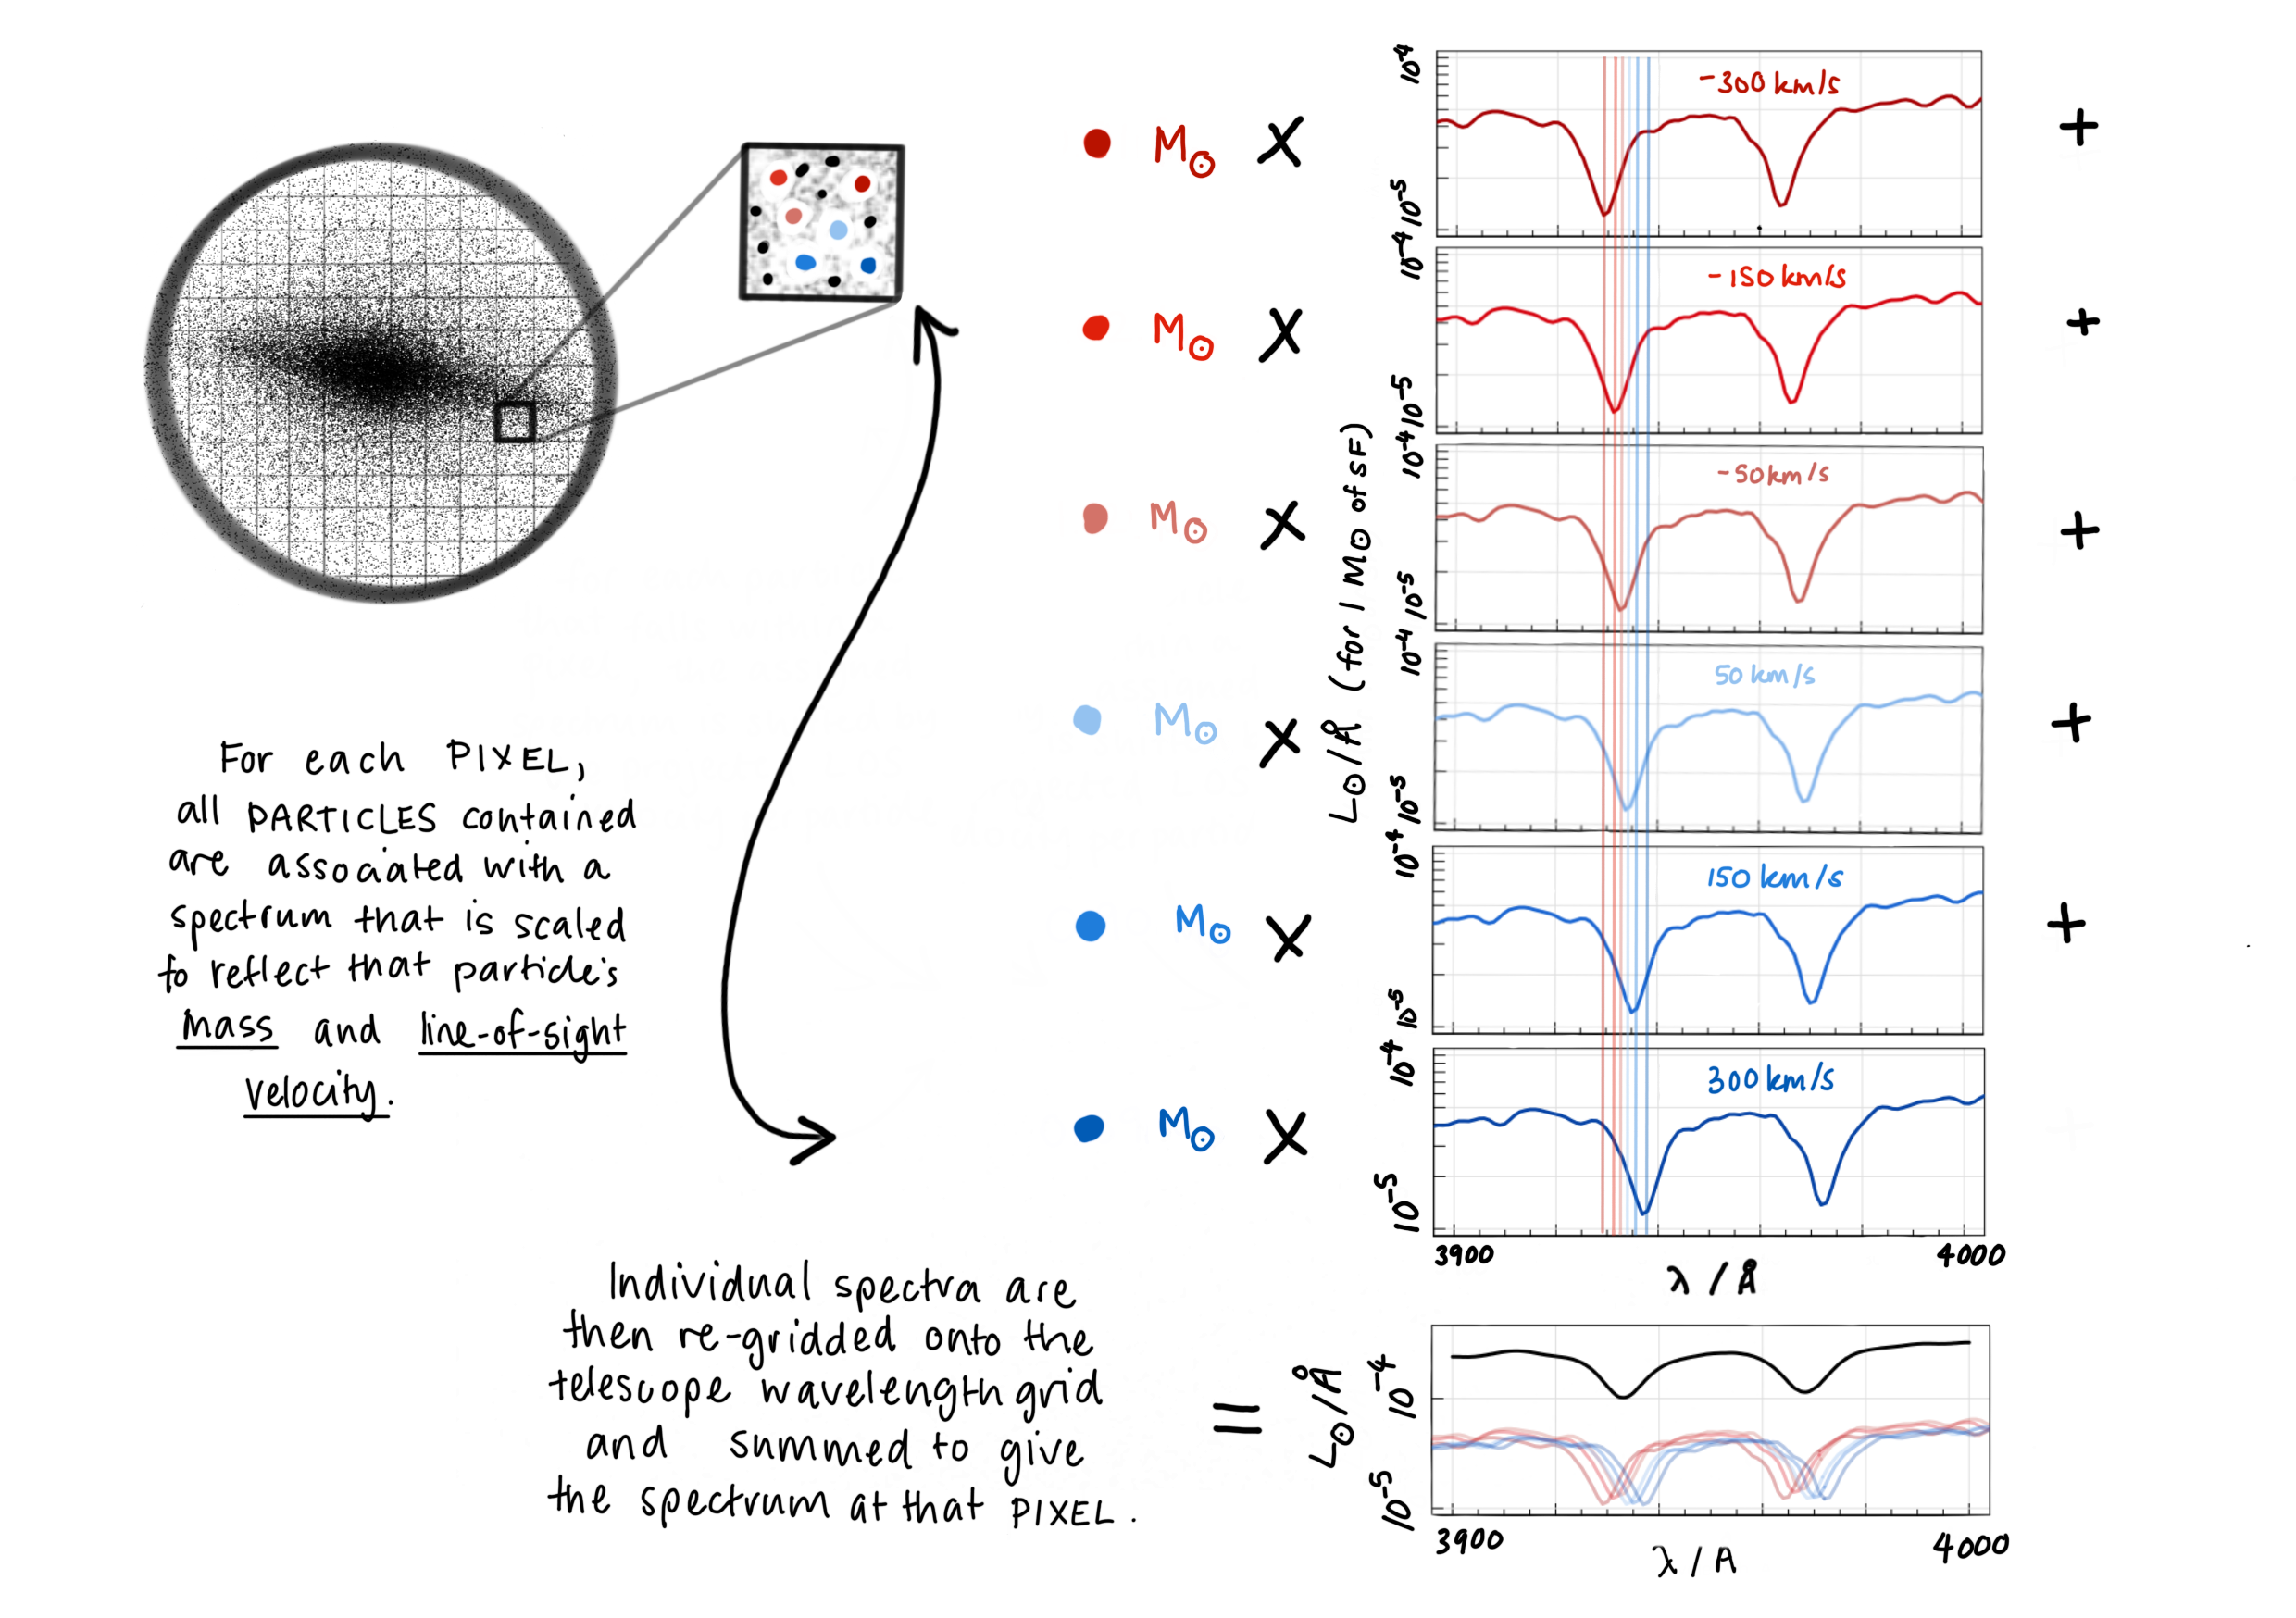
\includegraphics[keepaspectratio, width=14cm]{Figures/spectral_velocity_methodology.png}
    \caption{Method for constructing spectral data cubes. For the set of particles associated with each spaxel position across the field of view, we take the spectrum associated with each stellar particle, weight it by the initial mass of that star and then shift the spectrum in wavelength space to reflect that particle's line-of-sight velocity. Each spectrum in the pixel is then interpolated onto the wavelength range of the observing telescope and summed to give the overall spectrum at that spaxel position. The summed spectrum is finally convolved with the $\lambda_{\text{LSF}}$ of the observing telescope.}
    \label{fig:spectral_methodology}
\end{figure*}

Each stellar particle has been assigned a spectrum using the template described within the \makesimspinfile{} function in \cref{sec:make_simspin_file}. 
These spectra are at the resolution of the templates from which they have been drawn, e.g. with EMILES templates, these spectra will have a wavelength resolution of $\Delta \lambda = 0.9$\AA{} and a spectral resolution of 2.51\AA.
The template spectrum is weighted by the particle's stellar initial mass to give the luminosity as a function of wavelength.
    
We shift the wavelength labels to $\lambda_{\text{obs-z}} = \lambda (1 + z)$ to account for the input redshift of the system. 
Within each pixel, we then further shift the wavelength labels according to the LOS velocity of each individual particle, $\lambda_{\text{obs}} = \lambda_{\text{obs-z}} \text{exp}(v_{\text{LOS}}/c)$. 
At this stage we are still just modifying the raw spectral templates.

Once each template is both $z$-shifted and $v_{\text{LOS}}$-shifted, we then interpolate these spectra onto the wavelengths observed by the requested \telescope{}. 
This is done using a spline function in which an exact cubic is fitted using the method described by \citealt{Forsythe1977ComputerMethods}.
Next, the individual particle spectra are summed column-wise to produce the observed spectrum at that pixel. This procedure is repeated for every pixel within the FOV and then the spaxels are combined into a volume to construct a 3D data cube, with spatial dimensions in the $x$- and $y$-axes and wavelength information in the $z$-axes. 

If a point-spread-function (i.e. atmospheric blurring) has been specified in the \observingstrategy, we then perform a spatial 2D convolution across each $x-y$ plane in the cube.
The convolution kernel will have a shape and width as described by the \observingstrategy{}  in \S \ref{sec:observation}:
\begin{equation}
    F_{obs}(\lambda) = F(\lambda) \circledast PSF.
\end{equation}

Following the spatial convolution, we also need to convolve the summed spectrum with a Gaussian kernel, with width $\Delta \sigma_{\text{LSF}}$, mimicking the effects of the spectral resolution of the instrument, where $\Delta \sigma_{\text{LSF}}$ is the root-square of the difference between the telescope and the redshift-ed templates. 

\paragraph{Behaviour of the LSF}

\noindent The template spectra associated with a single particle have an intrinsic spectral resolution, $\lambda_{\text{LSF}}^{template}$. 
Of the templates included within this package, these resolutions range from 2.51 \AA{} - 3 \AA{} in the rest-frame.
This spectral resolution represents a ``minimum dispersion'' due to the instrument with which the template was observed or modelled. 
When the template spectrum is moved to greater redshift, the spectrum is stretched in wavelength space. 
When we wish to model a galaxy at redshift, $z$, the intrinsic spectral resolution of the templates must also be adjusted to this new redshift-ed spectrum. 
At higher redshift, the minimum dispersion we can detect with these templates becomes larger, as the wavelength space is broadened.

Hence, we must account for this when mimicking the effect of using our ``mock'' telescope with its spectral resolution, $\lambda_{\text{LSF}}^{telescope}$.
The value of this resolution is fixed by the telescope and is assumed constant with redshift. 
However, the templates which we have redshift-ed to some distance, $z$, will now have some intrinsic spectral resolution, $\lambda_{\text{LSF@z}}^{template} = \lambda_{\text{LSF}}^{template} (1 + z)$.
To match the spectral resolution of the observing telescope then, we only need convolve our templates with a Gaussian the root-square of the difference between the telescope and the redshift-ed templates, i.e. 

\begin{equation}
\Delta \lambda_{\text{LSF}} = \sqrt{(\lambda_{\text{LSF}}^{telescope})^2 - (\lambda_{\text{LSF@z}}^{template})^2}.
\label{eq:LSF}
\end{equation}

This is computed using the metadata information contained in the input SimSpin file. 
The user simply needs to specify the resolution of the observing telescope. 

Finally, we add the level of noise requested to each spectrum, as described in the \telescope{} function. 
The inverse variance of this noise ($1/noise^{2}$) is also returned to the user under the ``\texttt{variance\_cube}'' list element.
If no noise is requested, this list element will be returned the user with NULL. 

The resulting ``observed'' spectral cube is returned under the ``\texttt{spectral\_cube}'' list element. 
A summary of the run observation details are tabulated and returned under the list element ``\texttt{observation}''. 
At each pixel, we also measure a number of particle properties, including the total number of particles in each location, the total particle flux, the mean and standard deviation LOS velocity, the mean stellar age and mean stellar metallicity.  
This information is stored as an image returned to user under the list element ``\texttt{raw\_images}''.
All of these details can optionally be saved to a FITS file that contains each of these elements in subsequent HDU extensions for later processing with observational pipelines. 
Examples of this can be found at the documentation website.\footnote{\url{https://kateharborne.github.io/SimSpin/examples/examples}}

\subsubsection{Kinematic data cubes}
\label{sec:velocity_cubes}

If \texttt{method = "velocity"}, the \builddatacube{} function will return a data cube containing spatial information along the $x-$ and $y-$axes of the cube, and velocity information along the $z-$axis.  
A visual representation of this process is outlined in Figure \ref{fig:velocity_methodology}.

\begin{figure*}
    \centering
    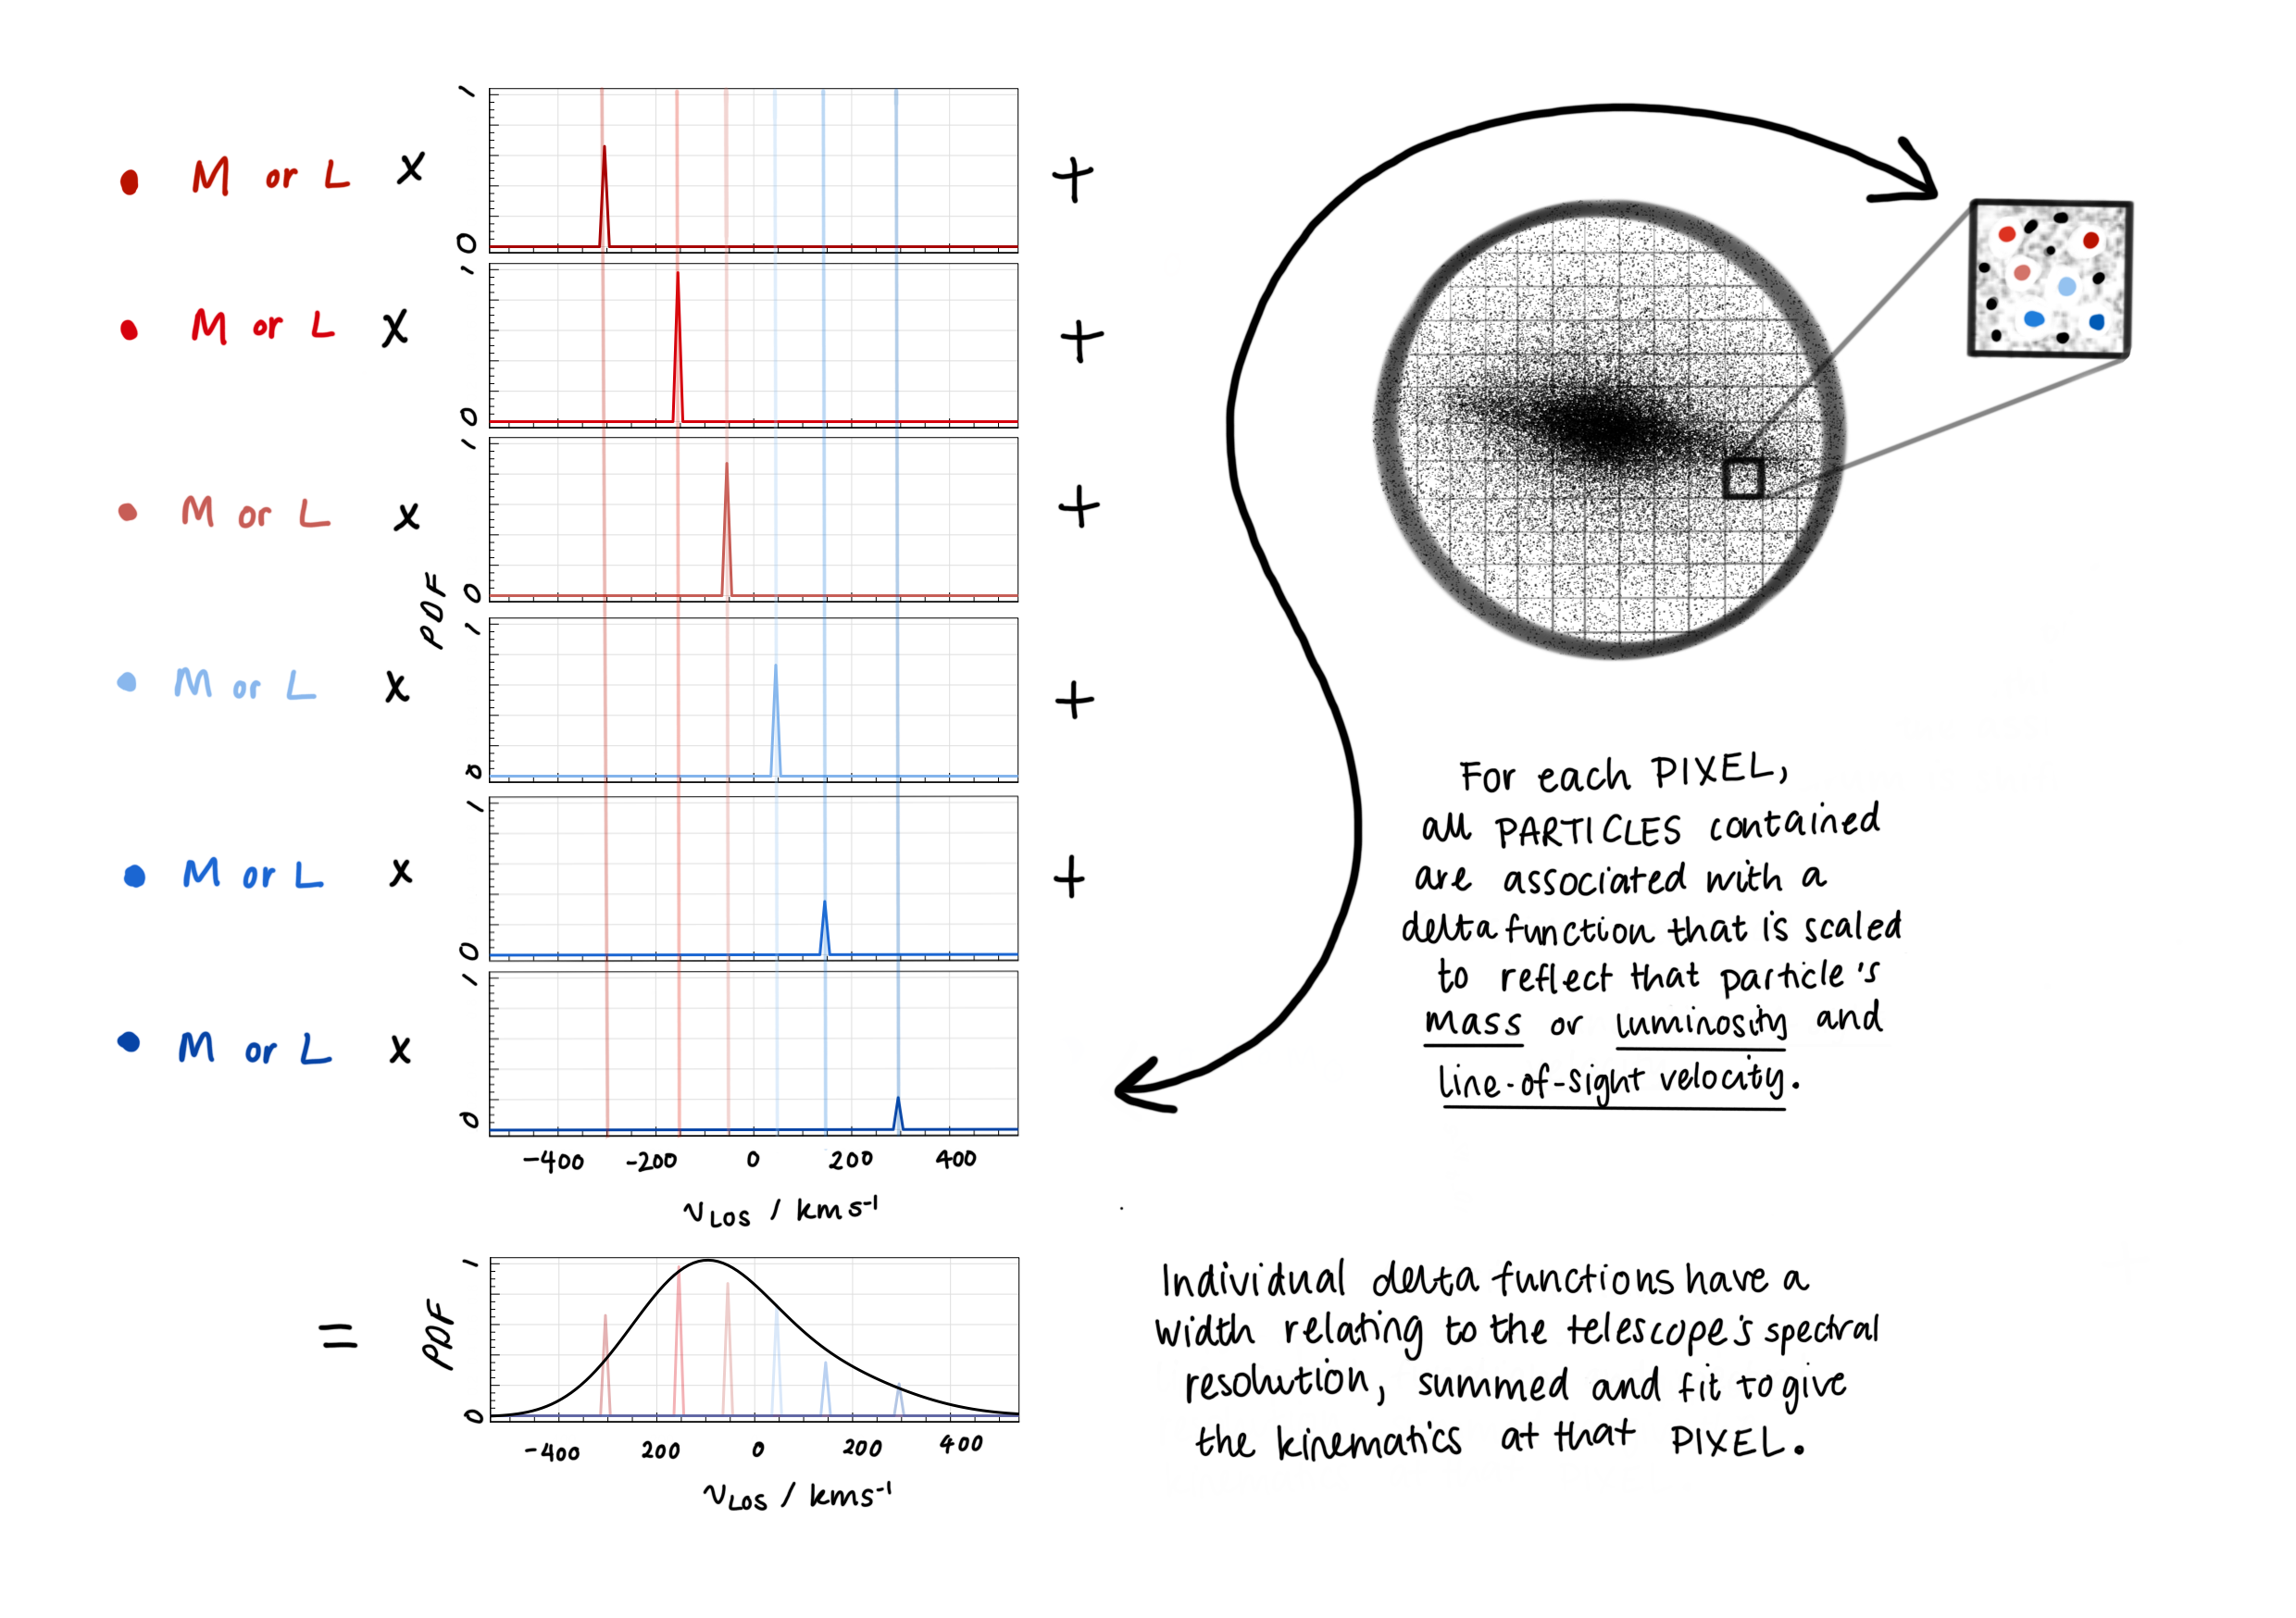
\includegraphics[keepaspectratio, width=14cm]{Figures/velocity_mode_methodology_v2.png}
    \caption{Method for constructing kinematic data cubes. At each pixel, the velocities of the contained particles are modelled as Gaussian distributions and binned into velocity channels that map back to the underlying spectral resolution of the observing telescope. These LOSVD's can be weighted by the underlying particle mass or luminosity depending on the settings selected at the \builddatacube{} stage.}
    \label{fig:velocity_methodology}
\end{figure*}

Given the wavelength and spectral resolution of the underlying telescope, we can compute the effective velocity sampling rate of a given instrument as:
\begin{equation}
\label{eq:vel_res}
    \Delta v = c \; \Delta \text{log}(\lambda)_{\text{min}},
\end{equation}
were $\lambda$ is the wavelength resolution of the given instrument, $\Delta \text{log}(\lambda)_{\text{min}}$ represents the smallest wavelength gap in log space and $c$ is the speed of light. 

As in the previous methodology, we can use the gridded FOV to perform the required mathematics on a pixel-by-pixel basis. 
For each pixel, we take each contained stellar particle. 
Each stellar particle has been assigned a spectrum using the template described within the \makesimspinfile{} function in \cref{sec:make_simspin_file}. 
This spectrum is multiplied by the initial mass of the stellar particle and re-gridded on the wavelength scale of a given telescope to give the luminosity at all wavelengths measured.
From this spectrum, the luminosity of that particle can be computed. 
Each particle also has a mass, which can be used to weight the kinematics in place of the particle luminosity when \texttt{mass\_flag = T}.

%We assume that the velocity of each particle has some uncertainty due to the resolution of the observing telescope. 
%This means that we can approximate the velocity of each particle as a Gaussian with mean equal to the line-of-sight velocity, $v_{los}$, and width equal to \br{the corresponding Nyquist scale of the associated resolution} as specified in \telescope. 
Each particle's velocity is binned along the velocity axis dependent on the wavelength (and associated velocity) resolution as specified in Equation \ref{eq:vel_res}. 
The height of this distribution is scaled to either the particle's luminosity in a given band or the mass of the particle. 
This leaves us with a line-of-sight velocity distribution (LOSVD) for each spatial pixel at the resolution of the respective \telescope. 
This process is repeated for every spatial pixel. 

At each pixel, as in the spectral mode case, we also measure a number of the raw particle properties including the total number of particles, the mean and standard deviation of the population of particle velocities, the mean stellar age and mean stellar metallicity. These are returned to the user as 2D named arrays embedded within the list element, ``\texttt{raw\_images}''.

If an atmospheric blurring is specified, convolution of the kernel selected and described in \S \ref{sec:observation} is performed across each spatial plane of the kinematic data cube following its construction, this time as a function of the velocity channels rather than wavelength channels:
\begin{equation}
    F_{obs}(v) = F(v) \circledast PSF.
\end{equation}

If requested, noise is added per spaxel as described in the \telescope{} function. 
We save a volume of the added noise as an inverse variance velocity cube ($1/noise^{2}$) and return this to the user under the list element ``\texttt{variance\_cube}''. 
The final, ``observed'' 3D array structure, containing spatial planes of the data in the $x-y$ at subsequent velocity channels along the $z-$axis, is returned to the user under the ``\texttt{velocity\_cube}'' list element. 

From this kinematic data cube, we also compute a number of ``\texttt{observed\_images}''. 
At each pixel in the cube, we now have a LOSVD sampled at the same resolution as the wavelength resolution of the telescope. 
This distribution is fit with a Gauss-Hermite function of the form:
\begin{equation}
    L(\omega, h_3, h_4) = \frac{1}{\sigma\sqrt{2\pi}} \; \text{exp}\left(-\frac{\omega^2}{2} \right) \left[ 1 + h_3 H_3 + h4 H_4 \right],
\end{equation}
where,
\begin{align}
    \omega &= \frac{v_i - V}{\sigma}, \\
    H_3 &= \frac{1}{\sqrt{6}} \left( 2\sqrt{2} \omega^3 - 3\sqrt{2} \omega \right), \\
    H_4 &= \frac{1}{\sqrt{24}}\left( 4 \omega^4 - 12 \omega^2 + 3 \right),
\end{align}
where $v_i$ is the observed velocity channels, $V$ and $\sigma$ are the first and second order moments of the LOSVD, $h_3$ and $h_4$ represent the expanded third and fourth moments of the Hermite polynomial \citep{vanderMarel1993AGalaxies, Cappellari2017ImprovingFunctions}.
This fit is performed using the quasi-Newton method published simultaneously by  Broyden, Fletcher, Goldfarb and Shanno in 1970 (known as BFGS) \citep{Broyden1970BFGS, Fletcher1970BFGS, Goldfarb1970BFGS, Shanno1970BFGS} using the \texttt{optim} minimisation provided in base R. 

We compute the observed LOS velocity, dispersion and higher-order kinematics $h_3$ and $h_4$ on a pixel by pixel basis through this fit. 
If a PSF has been specified in the \observingstrategy, this fit is performed on the spatially blurred cubes and the resulting images will have this blurring effect incorporated (unlike the raw particle properties, which will be returned as a summary of the underlying simulation). 
Each parameter is stored as a 2D array and returned to the user under the list element ``\texttt{observed\_images}''.
The residual of this fit to the LOSVD is also returned to give an understanding of how well these returned parameters describe the true underlying distribution.
This is also output as a 2D array under the same list element as the observed images. 

As in the spectral mode case, the returned observation can be written to a FITS file for later processing.
Each of the arrays in the list elements are saved to subsequent HDU extensions with explanatory names so that the raw and observed images can be distinguished (e.g. \texttt{OBS\_VEL} and \texttt{RAW\_VEL} for the observed LOSVD and the raw particle mean velocity images respectively).
These will be presented in a consistent format to the spectral FITS files, but with the velocity cube output under the \texttt{DATA} extension, with the necessary axes labels given the the header information. 

\subsubsection{Gas data cubes}
If \texttt{method = "gas"} or \texttt{"sf gas"}, the \builddatacube{} function will follow the kinematic data cube methodology, but only for the gas component (or gas classed as star-forming, in the later case) of the input model. 
As in \S\ref{sec:velocity_cubes}, this results in a data cube containing the spatial information about the gas distribution along the $x-y$ axes, with velocity information along the $z-$axis.

To distinguish between all gas and gas particles that are classed as star forming, we filter by the instantaneous star-formation rate.
These properties are commonly reported against each gas particle within the model and allow us to filter gas that has met the threshold for star formation. 

Beyond the focus on the gas component, rather than the stellar component, the process by which this cube is constructed is identical to above. 
The gas kinematics are weighted by the observed gas mass per pixel, rather than using a luminosity. 
This is equivalent to forcing \texttt{mass\_flag = T} in the stellar kinematic cube construction.
The mock observed kinematic images are constructed as above and we return the observed mass, velocity, dispersion, $h_3$ and $h_4$ images under the \texttt{"observed\_images"}
However, a number of additional raw particle properties are also included in the gas output. 

In addition to the raw gas mass per pixel, we record the mean mass-weighted instantaneous star formation rate, the mean gas metallicity, and the mean oxygen over hydrogen abundance ratio. 
The raw mass-weighted mean velocity and standard deviation are also returned in this \texttt{"raw\_images"} list under clearly named 2D arrays. 
A number of these images are shown for our example galaxy from the EAGLE simulation in Figure \ref{fig:simspin_v2} in the gas property maps on the right hand side.

In the future, we aim to incorporate the gas information at each pixel position within the spectral cube, through the addition of emission lines of appropriate ratio and kinematics.
This is currently beyond the scope of the code, due to the necessity to incorporate other features of realism such as the attenuation and re-emission due to dust which is currently beyond the resolution limits of the majority of simulations. 

\section{RESULTS}

\subsection{Comparison of spectral and kinematic cubes}
\label{sec:cs1}

A kinematic data cube should mimic the kinematic information included within a full spectral cube. 
Here, we present a series of tests to ensure the similarity of these products using two high-resolution galaxy models.
One model represents a disk galaxy with highly coherent, rotational support.
The other represents an elliptical galaxy with highly dispersive support. 
At these extremes, we hope to identify any systematic offsets between the kinematic cubes and spectral cubes as a function of the underlying model. 

These high-resolution $N$-body models have been constructed using the initial conditions code \texttt{GalIC} \citep{Yurin2014AnEquilibrium} and evolved in a smooth analytic potential using a modified version of \texttt{Gadget2} \citep{Springel2005TheGADGET-2}. 
Each galaxy contains $6.5 \times 10^{6}$ particles, each of mass $1 \times 10^{4}$ M$_{\odot}$. 

The elliptical system is modelled as a spherically symmetric model with density profile described by:
\begin{equation}
    \rho(r) = \frac{M}{2 \pi} \frac{a}{r(r+a)^3},
\end{equation}
where $a$ is the scale factor given by,
\begin{equation}
    a = \frac{r_{200}}{c}\sqrt{2 \left[ \text{ln}(1 + c) - \frac{c}{(1 + c)} \right]},
\end{equation}
where $r_{200}$ and $c$ is the concentration of the distribution. 

The disk model has been initialised with an exponential radial profile and sech$^{2}$-profile in the vertical height, described by:
\begin{equation}
    \rho(R,z) = \frac{M_*}{4 \pi z_{0} h^2}\text{sech}^2\left( \frac{z}{z_{0}} \right)\text{exp}\left( - \frac{R}{h} \right)
\end{equation}

The velocity profiles of these structures are initialised using the optimisation procedure outlined in \citealt{Yurin2014AnEquilibrium}. 
We allow these systems to evolve in an analytic potential for 10 Gyr using \texttt{Gadget2}. We outline the procedure for each test below.

We begin by generating three \simspin{} files. 
As these are $N$-body models, we must assign each particle a stellar age and metallicity (such that an appropriate stellar template can be assigned). 
We produce two \simspin{} files with identical particle ages and metallicities in order to examine both the variation of the underlying kinematic model (i.e. bulge vs. disk) with consistent underlying spectra:
    
\begin{lstlisting}[basicstyle=\fontsize{6}{8}\selectfont\ttfamily]
make_simspin_file(filename = "disk_model.hdf5", 
                  disk_age = 5, 
                  disk_Z   = 0.024, 
                  template = "EMILES", 
                  output = "disk_age05_Z024.Rdata")
    
make_simspin_file(filename  = "bulge_model.hdf5", 
                  bulge_age = 5, 
                  bulge_Z   = 0.024, 
                  template  = "EMILES",
                  output = "bulge_age05_Z024.Rdata")
                  
\end{lstlisting}
    
The final \simspin{} file contains more realistic stellar ages and metallicities for their component, with older, more metal poor stars present in the elliptical system and younger, more metal rich stars in the disk galaxy. 
This allows us to examine the effect of varied stellar templates on the comparison between spectral and kinematic data cubes.

\begin{lstlisting}[basicstyle=\fontsize{6}{8}\selectfont\ttfamily]
make_simspin_file(filename  = "bulge_model.hdf5", 
                  bulge_age = 10, 
                  bulge_Z   = 0.001, 
                  template  = "EMILES",
                  output = "bulge_age10_Z001.Rdata")
                  
\end{lstlisting}

We build two versions of each of these files. 
One is prepared using the \textsc{EMILES} templates \citep{Vazdekis2016UV-extendedGalaxies}, which have both higher wavelength and spectral resolution parameters than the alternative \textsc{GalexEV} models \citep{Bruzual2003Stellar2003} from which we prepare the second \simspin{} file.  

These \simspin{} files are used for the following tests in an effort to evaluate the consistency between our two mock observing methods.
In each case, we generate a kinematic data cube and a spectral data cube.
These cubes have identical observing conditions, i.e. projected distance, observed projection angle on the sky, field of view, etc. 
The spectral cube is then fit using pPXF, with the EMILES spectra used as fitting templates.
We then compare the kinematic maps produced through the penalised pixel fitting method and our kinematic cubes. 
With the two versions of SimSpin file (\textsc{EMILES} and \textsc{GalexEV}), we can examine consistency across a variety of spectral qualities.
Within each test, we can further turn the dials of the \telescope{} and \observingstrategy{} functions to explore the reliability of the results with respect to the LSF, spatial and spectral resolution and seeing.

Selected properties are described in each of the case studies below. 
We have comparison figures for each test contained in the supplementary material at the end of the paper, though a summary of these is also presented at the end of the results section. 
A walk-through of code used to generate these examples can also be found at the SimSpin website. 

\subsubsection*{Test 1: Observations of intrinsic template spectral resolution at low redshift. \\ }

We would like to ensure that, in the simplest regime where no line-spread-function convolution is applied and negligible redshift is applied to the spectral cubes, a kinematic data cube and a spectral data cube fit with pPXF will return consistent answers. 
In essence, this tests that the velocity-shift added to each particle's spectrum is working appropriately. 
This is done for all three examples (the young disk, young bulge and old bulge). 
We use different \telescope{} configurations for the EMILES and \textsc{GalexEV} cubes to suit the different resolution constraints for these spectra, and to explore the robustness of the comparison to different configurations of the telescope. 

This is done using the following telescope parameters for the EMILES and BC03hr cubes respectively:
\begin{lstlisting}[basicstyle=\fontsize{6}{8}\selectfont\ttfamily]
telescope(type = "IFU", signal_to_noise = 30, 
          lsf_fwhm = 0, wave_res = 1.04,
          aperture_shape = "circular", fov = 15,
          spatial_res = 0.5)

telescope(type = "IFU", signal_to_noise = 30, 
          lsf_fwhm = 0, wave_res = 3, 
          aperture_shape = "hexagonal", fov = 17,
          spatial_res = 0.7)
\end{lstlisting}

\noindent The same observing strategy is used for all observations:
\begin{lstlisting}[basicstyle=\fontsize{6}{8}\selectfont\ttfamily]
observing_strategy(dist_kpc_per_arcsec = 0.3, 
                   inc_deg = 60, blur = F)
\end{lstlisting}

In this test, we force SimSpin to generate a spectral cube at the intrinsic template spectral resolution by requesting a telescope with a $\lambda_{\text{LSF}}^{telescope} = 0$ \AA.
This will cause the code to issue a warning that the templates used have insufficient resolution to construct such an observation, but will produce the output spectral cube never-the-less. 

\begin{figure}
    \centering
    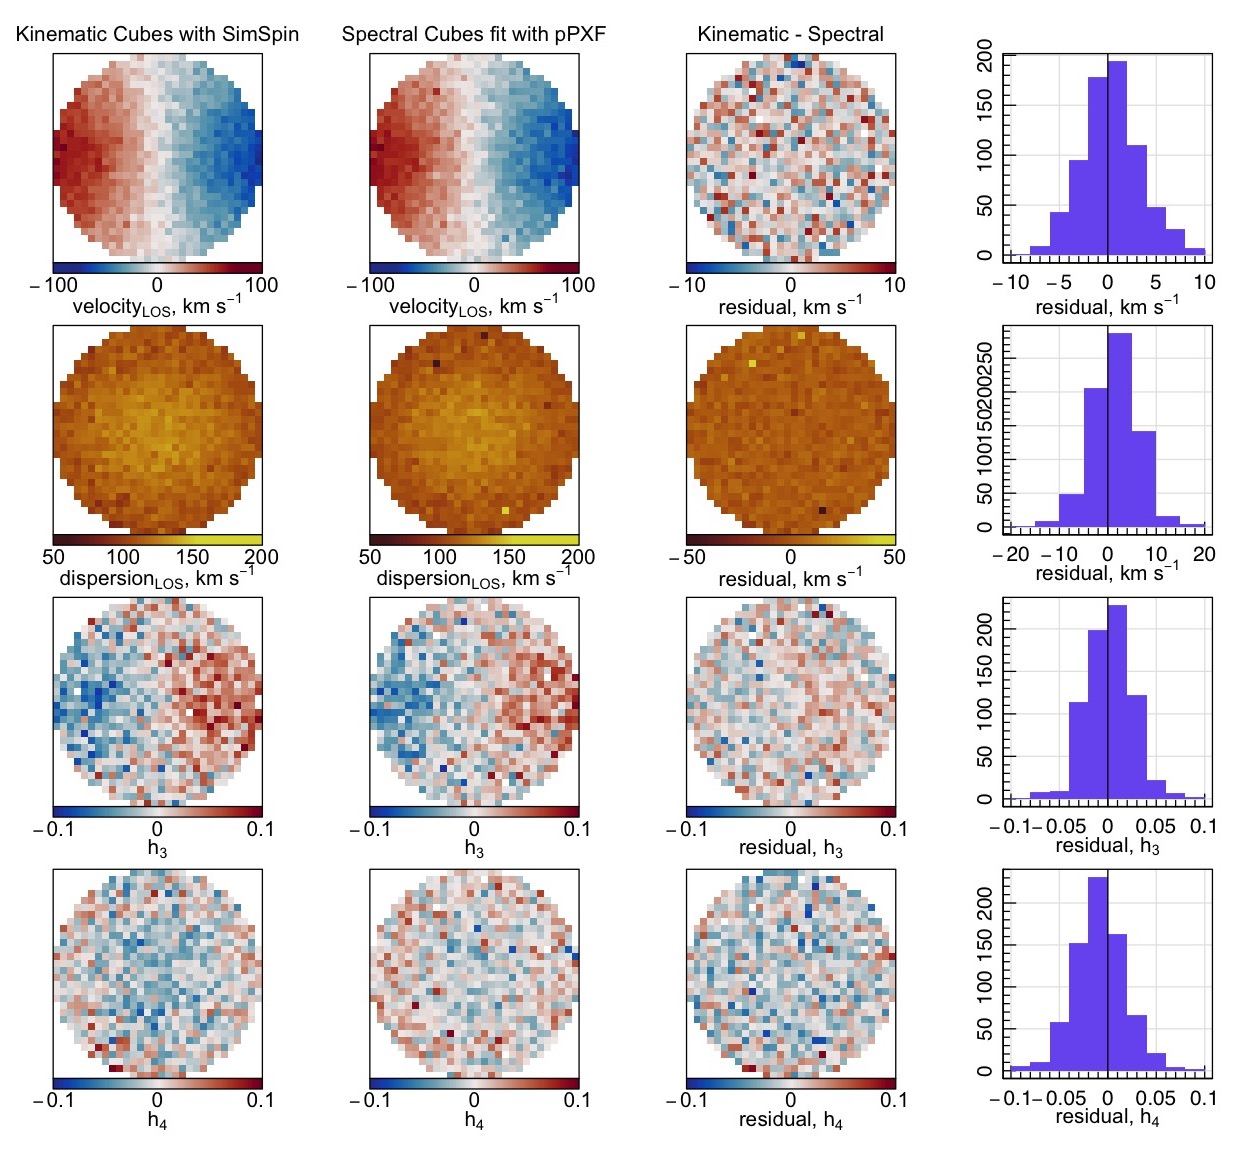
\includegraphics[keepaspectratio, width=8cm]{Figures/cs1_disk_velocities_lowz_EMILES.jpeg}
    \caption{Case Study 1: The disk model built with EMILES templates observed with an intrinsic telescope resolution of  $\lambda_{\text{LSF}}^{telescope} = 0$ \AA{} at a low redshift distance of $z = 0.0144$. Here we compare the output kinematic cubes to the kinematics fit with pPXF.}
    \label{fig:cs1_disk_EMILES}
\end{figure}

\begin{figure}
    \centering
    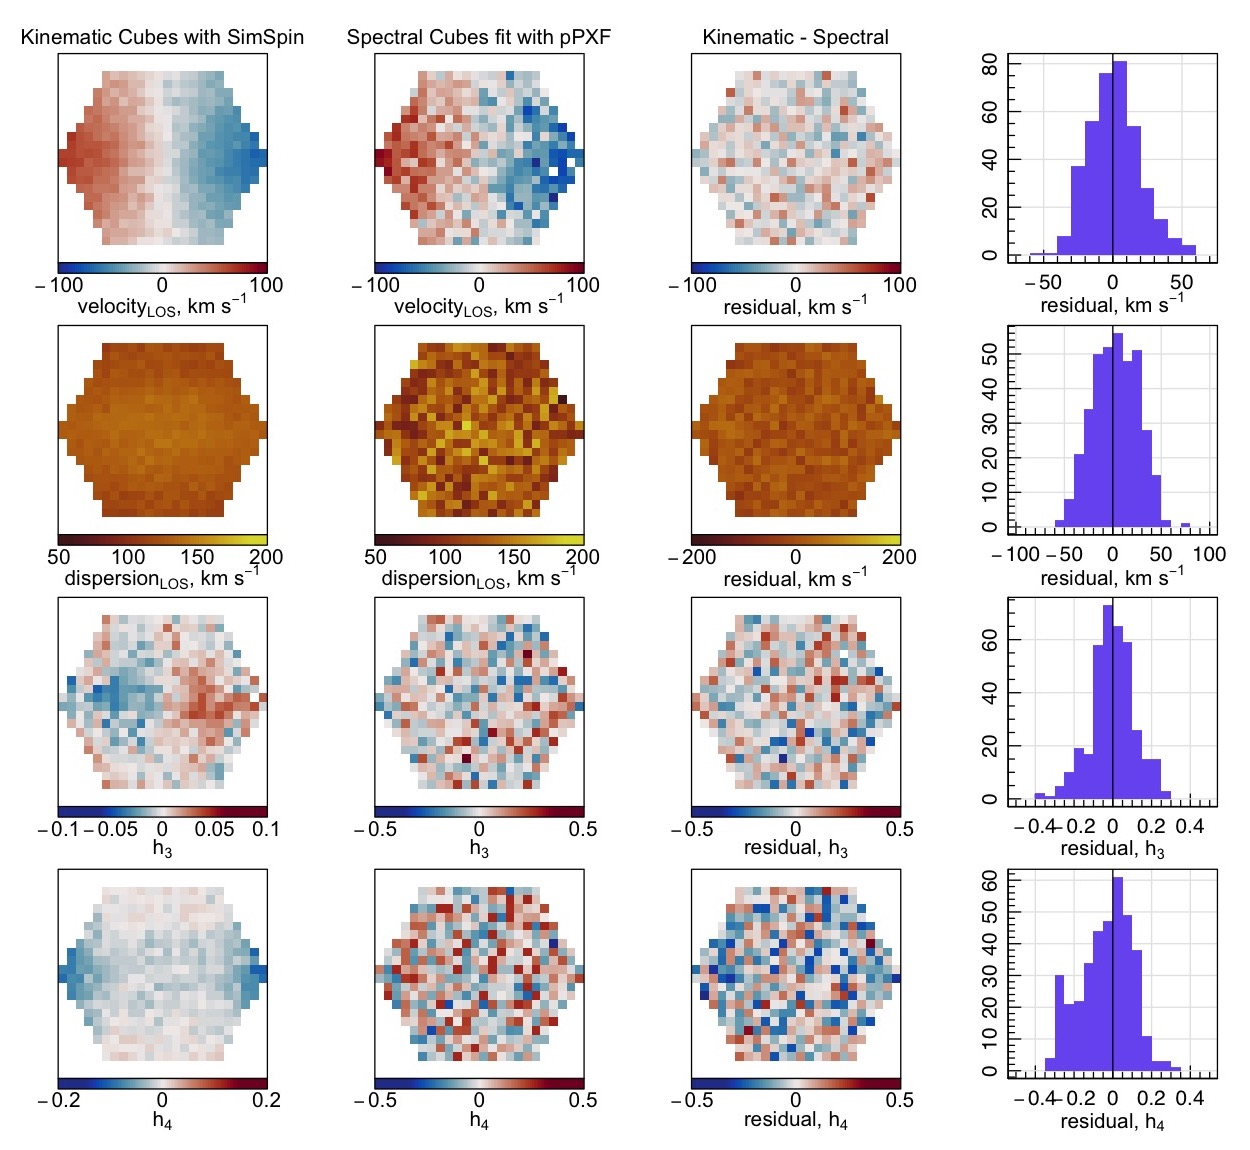
\includegraphics[keepaspectratio, width=8cm]{Figures/cs1_disk_velocities_lowz_BC03.jpeg}
    \caption{Case Study 1: The disk model built with BC03 templates observed with an intrinsic telescope resolution of  $\lambda_{\text{LSF}}^{telescope} = 0$ \AA{} at a low redshift distance of $z = 0.0144$. Here we compare the output kinematic cubes to the kinematics fit with pPXF.}
    \label{fig:cs1_disk_BC03}
\end{figure}

It is important to remember that the underlying templates used to construct the observed galaxy do have some intrinsic line-spread-function, as shown in Table \ref{tab:templates}.
Hence, when using spectral templates to fit the SimSpin spectral cubes with pPXF, it is important that we do match the fitting templates to the true underlying LSF, which is dependent on the templates from which the cube has been made ($\lambda_{\text{LSF}}^{templates} = 2.51$ \AA{} in the case of EMILES SimSpin cubes and $\lambda_{\text{LSF}}^{templates} = 3$ \AA{} in the case of \textsc{GalexEV} SimSpin cubes). 
When performing the pPXF fit using the EMILES templates to fit the model spectra, we do convolve the fitting templates with the root-square difference between the \textsc{GalexEV} and EMILES line spread function (i.e. $\sqrt{3^{2} - 2.51^{2}} = 1.64$\AA{} and $\sqrt{2.51^{2} - 2.51^{2}} = 0$\AA), due to the fact that the intrinsic templates from which the mock observation has been built have a greater LSF than the templates used to perform the fit. 

We compare the output of the pPXF run in this case to a kinematic data cube run using the same parameters, but this time with \texttt{method = "velocity"}. 
We expect that the observed kinematics will be consistent within the noise. 
The resulting comparison can be seen visually for our disk model in Figures \ref{fig:cs1_disk_EMILES} and \ref{fig:cs1_disk_BC03}. 
Similar plots for each of the models built for these tests can be found in \ref{app:cs1}.
Visually, it is clear that the EMILES spectral cube comparison in Figure \ref{fig:cs1_disk_EMILES} is much more consistent than the BC03 spectral cube comparison in Figure \ref{fig:cs1_disk_BC03}. 
However, in both cases the residual distributions are centred around zero. 
In the recovery of the kinematics in the \textsc{GalexEV} example, we struggle to find a sufficiently good fit, with the mean $\chi^2$/DOF averaging 4.8, as opposed to the EMILES comparison value of 1.2. 
We believe this is due in part to template mismatch. 

\begin{figure}
    \centering
    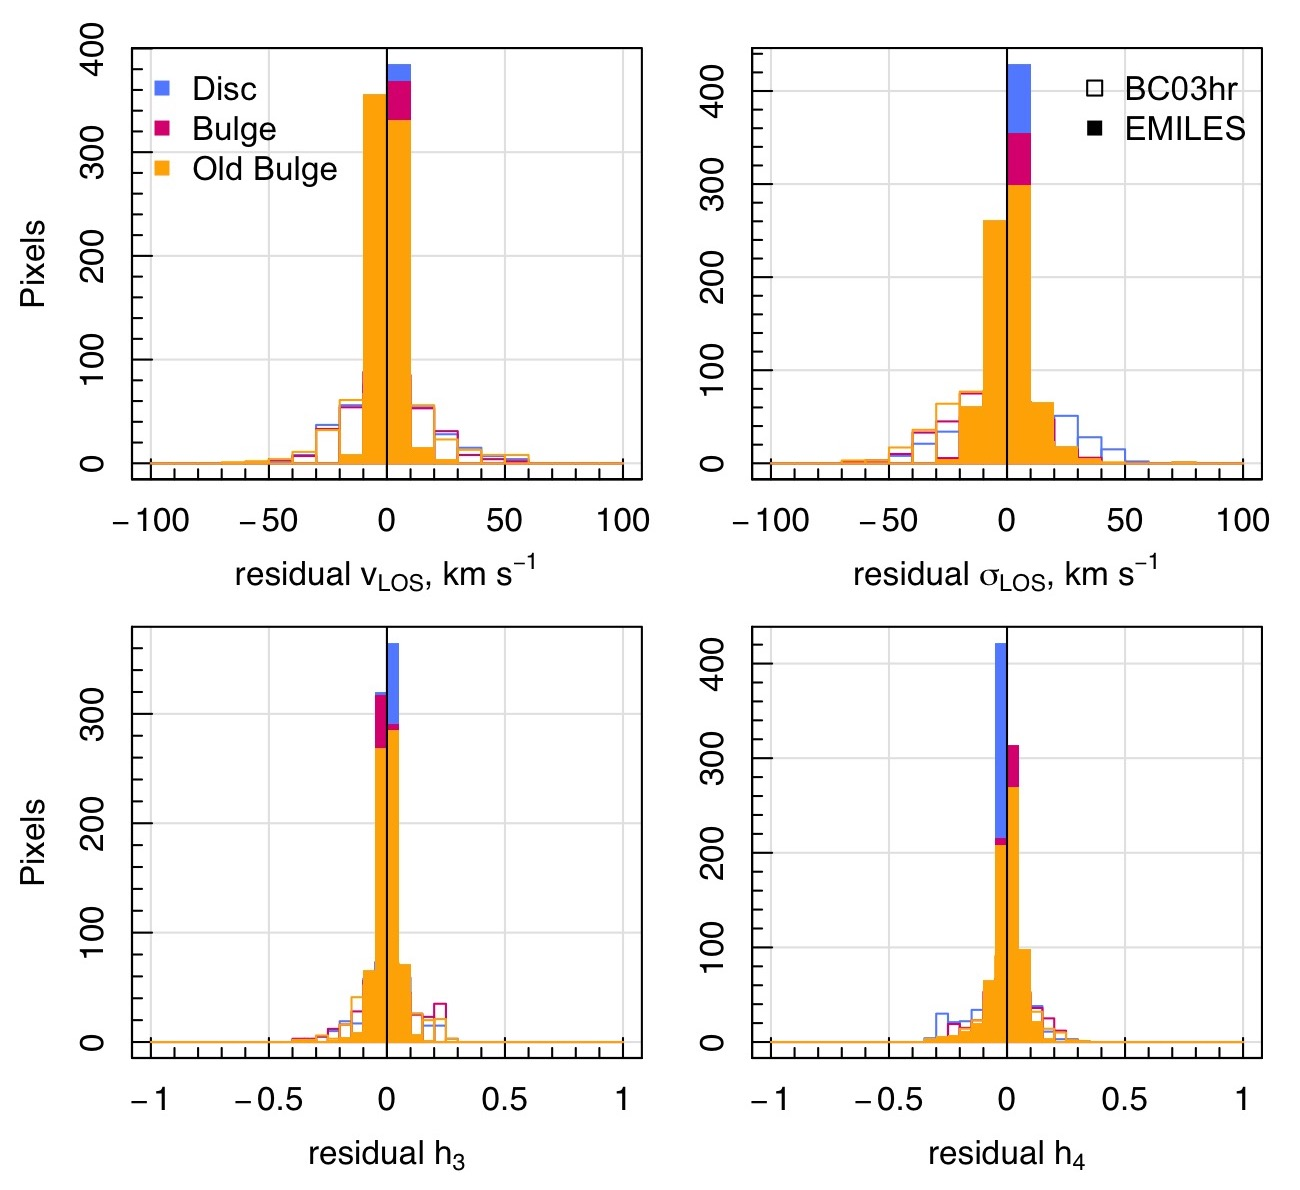
\includegraphics[keepaspectratio, width=8cm]{Figures/cs1_histograms.jpeg}
    \caption{Case Study 1: The residual differences between the kinematic observations and the spectral fits in case study 1 for the $v_{\text{LOS}}$, the $\sigma_{\text{LOS}}$, $h_3$ and $h_4$ for each of the models (disc, bulge, and old bulge in blue, pink and yellow respectively). The bold colours show the residual relationship for the EMILES cubes, while the outline demonstrates the residuals for the BC03hr cubes. All are nicely centred around zero as we would expect, though we do see significantly broader distributions for the BC03hr models in comparison to the EMILES models.}
    \label{fig:cs1_hist}
\end{figure}

In Figure \ref{fig:cs1_hist}, we show the residual differences between the kinematic and spectral cubes as a histogram for each model and spectral template set. 
This allows us to directly compare the differences between spectral cubes built with the EMILES and \textsc{GalexEV} templates.
At low redshift and with no additional LSF effects, we see that the two methods (\texttt{"spectral"} and \texttt{"velocity"}) compare quite nicely, with all resulting residuals centred around zero.
As noted visually from the kinematic maps, there is a broader difference between the returned kinematics for the \textsc{GalexEV} SimSpin cubes fit with the EMILES templates through pPXF.


%We further note here that, despite the very low redshift of the observation at $z=0.0144$, the fits with pPXF do require that we bring all spectra back to rest-frame before performing the kinematic fit.
%In \ref{app:rest}, we demonstrate the increased dispersion measured when this step is not followed, and we allow the velocity to be found through the spectral fit alone.
%We caution that it is best to shift all observed spectra back to rest-frame before performing the spectral fit through pPXF. 

%Finally, we examine specifically the residuals of the dispersion measure as a function of radius, the number of particles per pixel, and the $\chi^2$/DOF value from the pPXF fit.
%This is shown in Figure \ref{fig:cs1_res}.
%Clearly, we see that the EMILES models have a tighter spread about the zero line for all properties. 


%\begin{figure}
%    \centering
%    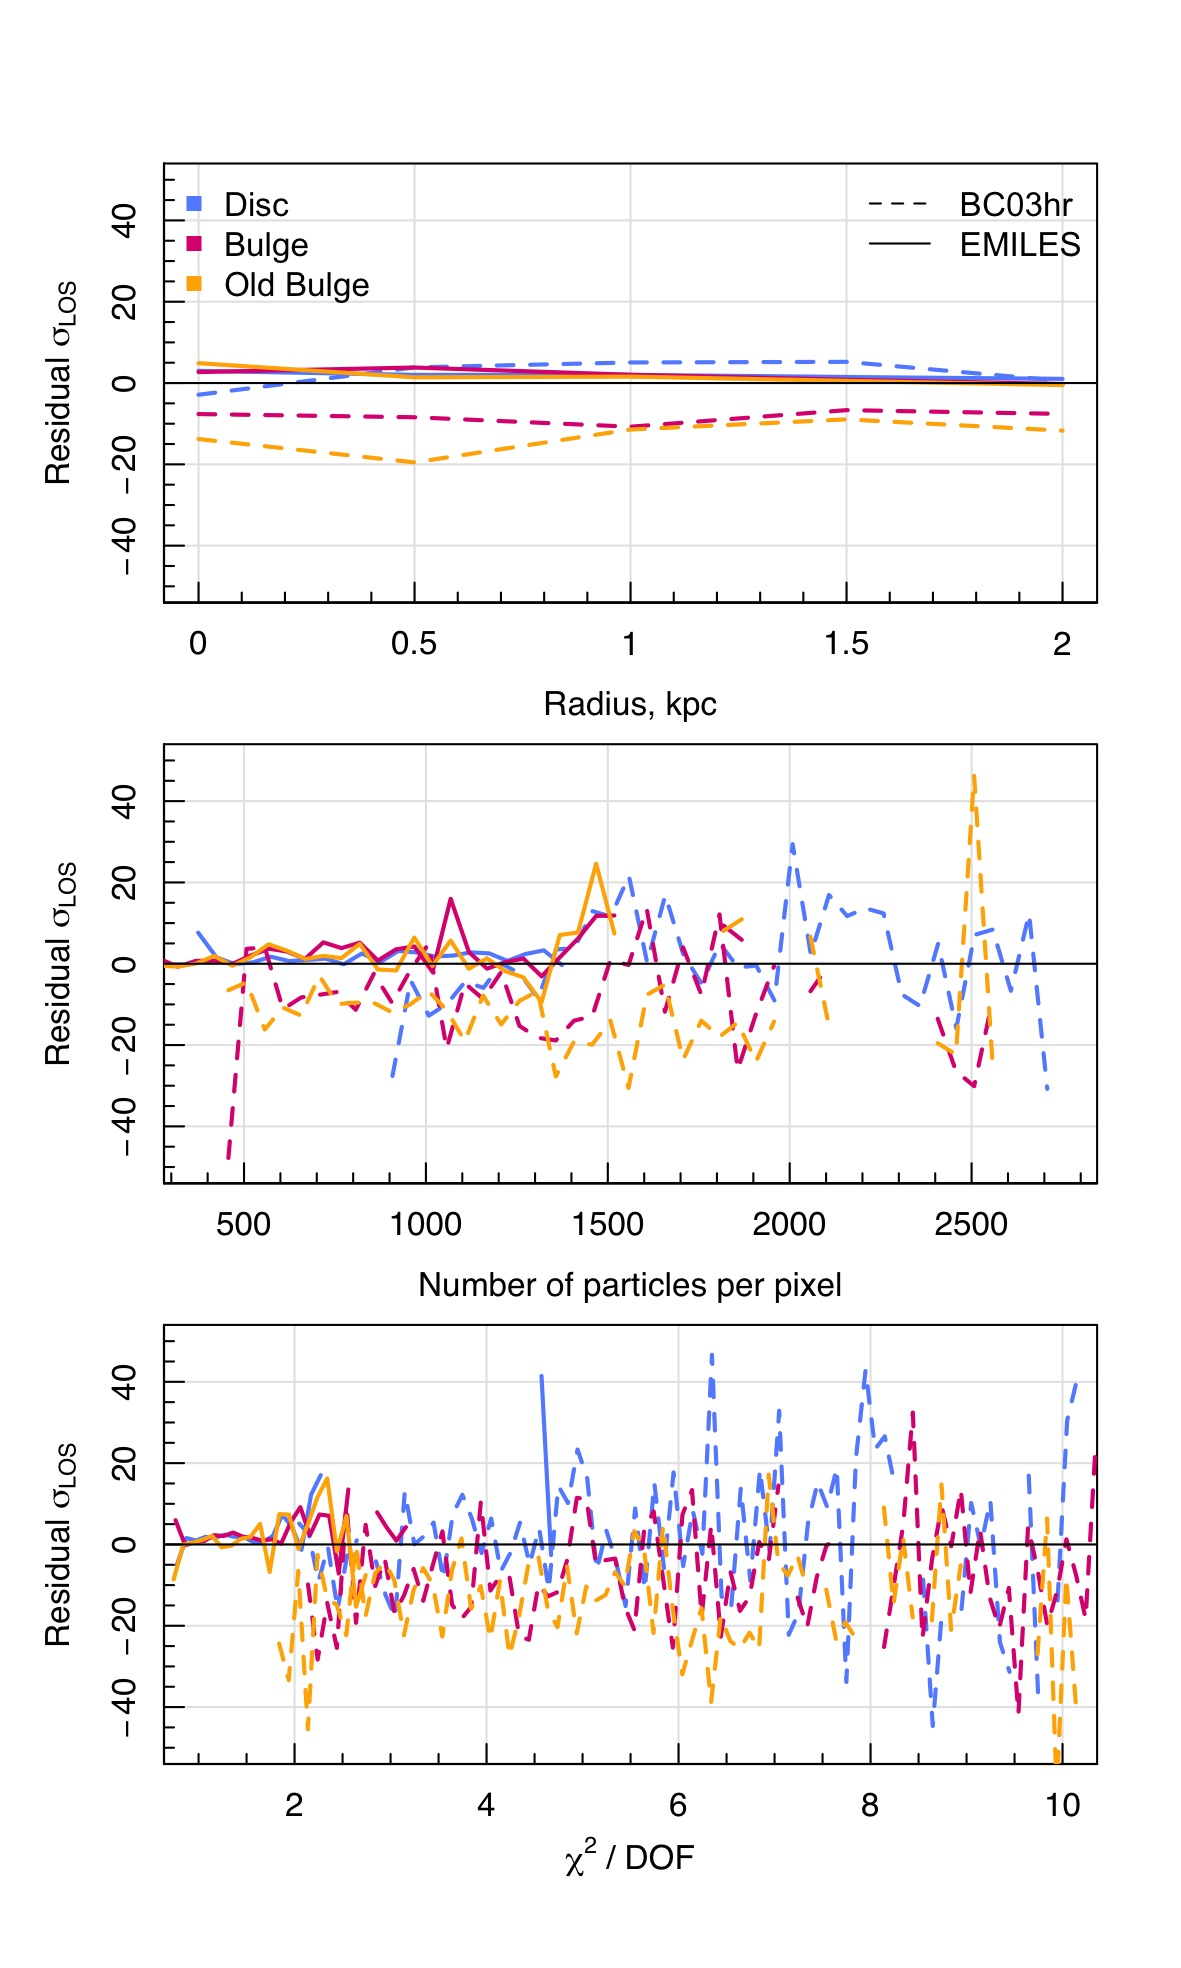
\includegraphics[keepaspectratio, width=8cm]{Figures/cs1_dispersion_residuals.jpeg}
%    \caption{The residual differences between the kinematic observations and the spectral fits for the $\sigma_{\text{LOS}}$, for each of the models (disc, bulge, and old bulge in blue, pink and yellow respectively) as a function of radius (top), number of particles per pixel (centre) and the $\chi^2$/DOF of the pPXF fit (bottom). The bold colours show the residual relationship for the EMILES cubes, while the dashed demonstrates the residuals for the BC03hr cubes. The strongest driver of the residual in these cases appears to be the goodness of fit, where the scatter about zero increases with larger values of $\chi^2$/DOF.}
%    \label{fig:cs1_res}
%\end{figure}

\subsubsection*{Test 2: Observations of intrinsic template spectral resolution at high redshift. \\ }

Following the success at low redshift, where we tested that spectra are shifted in wavelength space effectively, we next consider the effect of projecting the galaxies to larger distances. 
In this study, we use the same telescope definitions as in Test 1, keeping the templates from which the cubes are built at their intrinsic resolution using $\lambda_{\text{LSF}}^{telescope} = 0$ \AA, but modifying the observing strategy as follows:
\begin{lstlisting}[basicstyle=\fontsize{6}{8}\selectfont\ttfamily]
observing_strategy(dist_z = 0.3, 
                   inc_deg = 60, blur = F)
\end{lstlisting}

Here, we examine whether the red-shifting module is working effectively in both methods and still produces equivalent results between the \texttt{spectral} and \texttt{velocity} cubes.
We build both a spectral and velocity cube of each of the simulations with these specifications.
The resulting spectral cubes are fit using pPXF to find the observed spectral kinematics and the maps are compared with their \texttt{method = "velocity"} counterparts. 

\begin{figure}
    \centering
    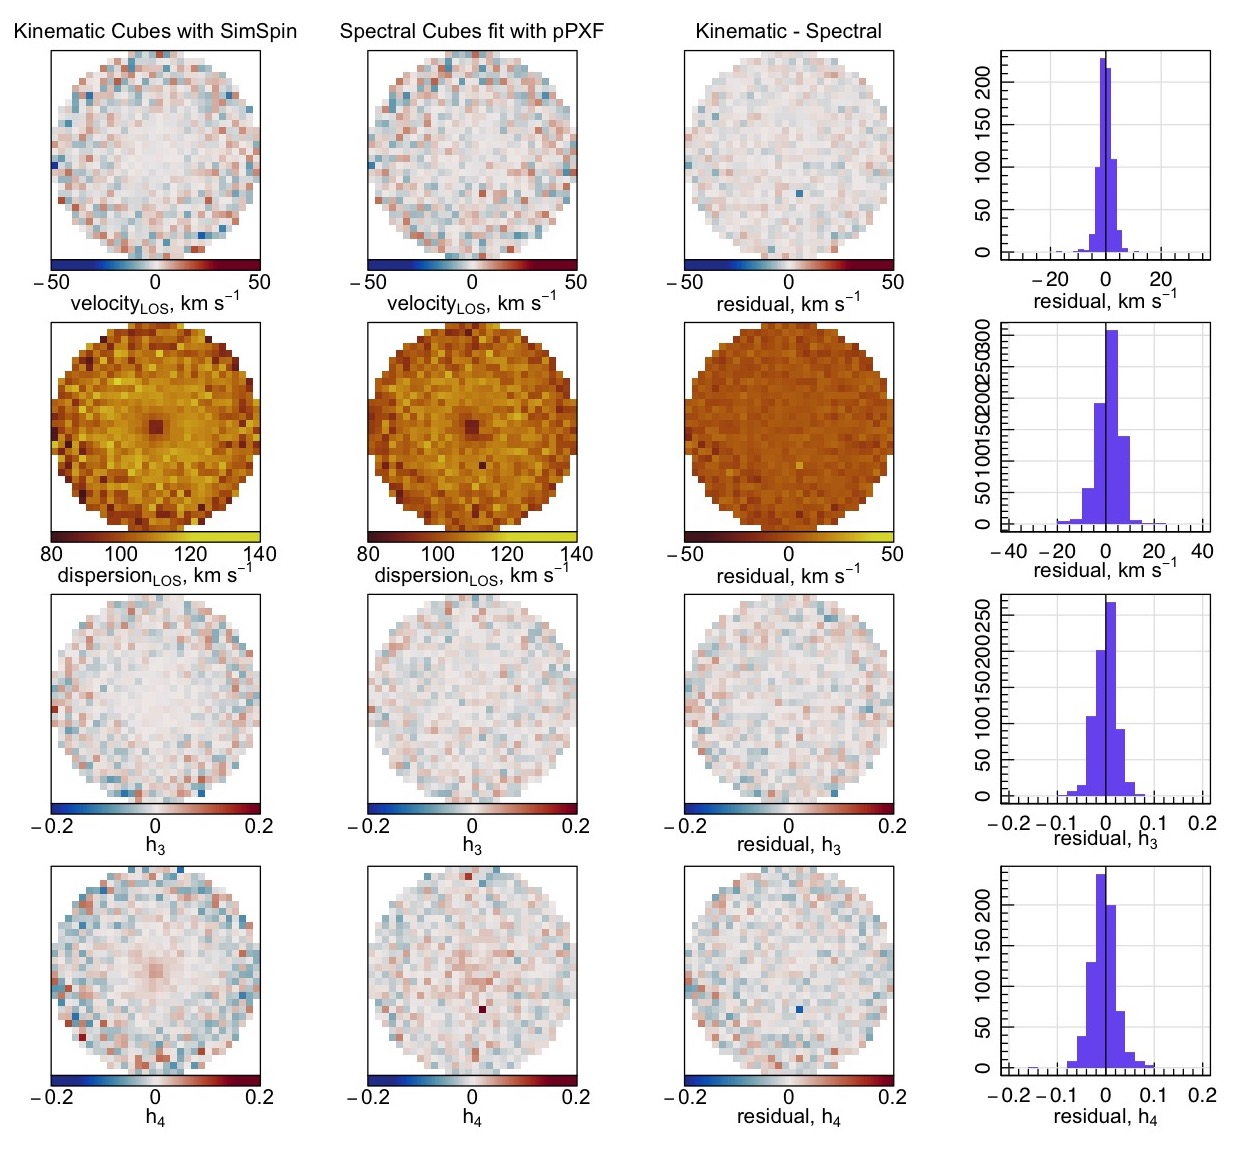
\includegraphics[keepaspectratio, width=8cm]{Figures/cs2_bulge_velocities_highz_EMILES.jpeg}
    \caption{Case Study 2: The bulge model built with EMILES templates observed with an intrinsic telescope resolution of  $\lambda_{\text{LSF}}^{telescope} = 0$ \AA{} at a high redshift distance of $z = 0.3$. Here we compare the output kinematic cubes to the kinematics fit with pPXF.}
    \label{fig:cs2_bulge_EMILES}
\end{figure}

\begin{figure}
    \centering
    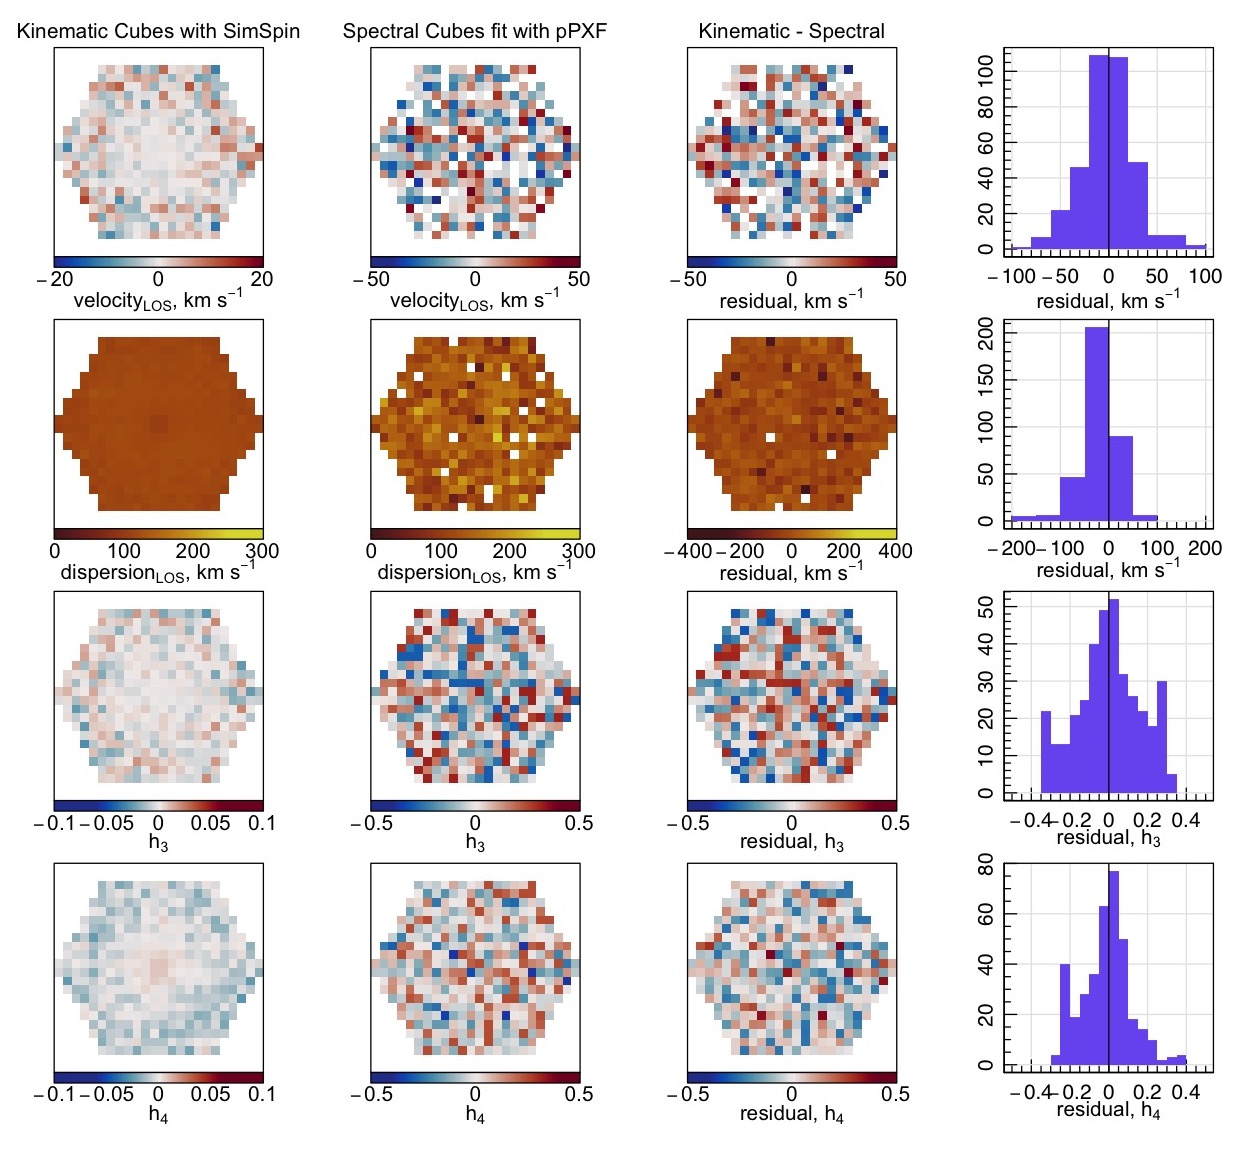
\includegraphics[keepaspectratio, width=8cm]{Figures/cs2_bulge_velocities_highz_BC03hr.jpeg}
    \caption{Case Study 2: The bulge model built with BC03 templates observed with an intrinsic telescope resolution of  $\lambda_{\text{LSF}}^{telescope} = 0$ \AA{} at a high redshift distance of $z = 0.3$. Here we compare the output kinematic cubes to the kinematics fit with pPXF.}
    \label{fig:cs2_bulge_BC03}
\end{figure}

As in the previous test, we produce visual analysis by comparing the kinematic maps for each model, as shown in Figures \ref{fig:cs2_bulge_EMILES} and \ref{fig:cs2_bulge_BC03}.
This time, we demonstrate using the bulge model, but provide the images for every model tested in \ref{app:cs2}.
We successfully recover kinematic details in the EMILES built images in Figure \ref{fig:cs2_bulge_EMILES}.  
However, we find that it is much more difficult to get a successful fit for the BC03 spectral cubes through pPXF. 
The direct comparison between the two is clearly demonstrated in the histograms in Figure \ref{fig:cs2_hist}.
At the wavelength resolution of 3 \AA, as is run for the \textsc{GalexEV} SimSpin cubes, we find that it is especially difficult to recover the higher order kinematics.

\br{Following fits from Caro and Sam, I'm hoping that we can improve the quality of these fits as they are quite poor but visibly so from the output spectra fits and $\chi^2$...}

\begin{figure}
    \centering
    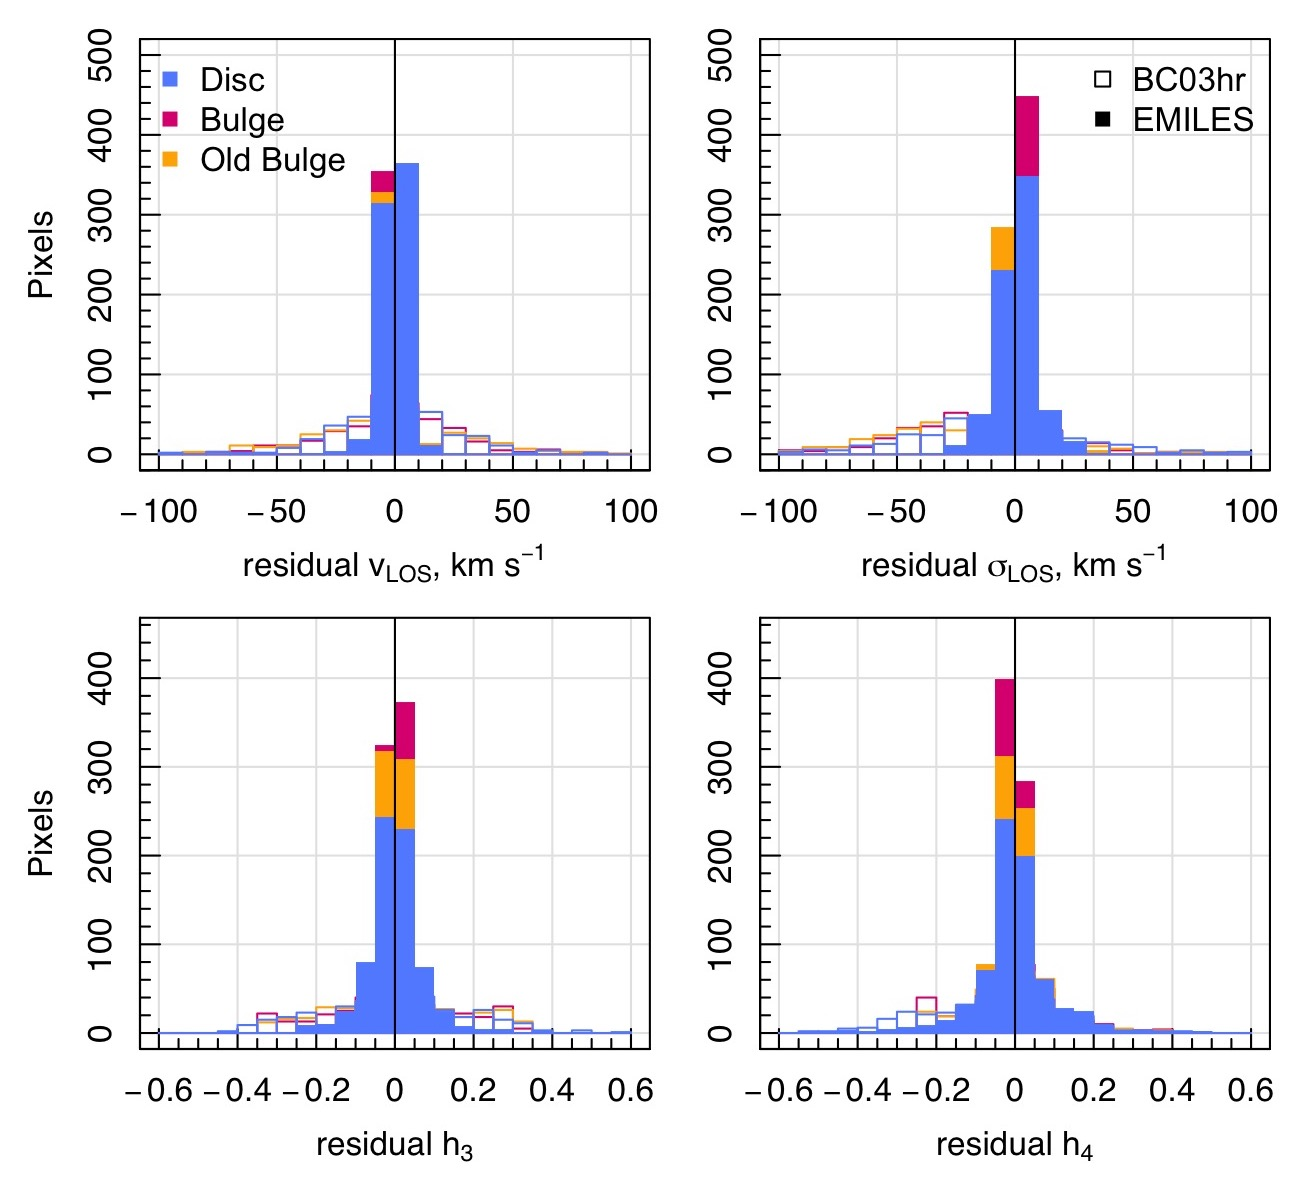
\includegraphics[keepaspectratio, width=8cm]{Figures/cs2_histograms.jpeg}
    \caption{Case Study 2: The residual differences between the kinematic observations and the spectral fits as in Figure \ref{fig:cs1_hist}, but for case study 2. Again, we find that all distributions are nicely centred around zero as we would expect, though we do see significantly broader distributions for the BC03hr models in comparison to the EMILES models.}
    \label{fig:cs2_hist}
\end{figure}

\subsubsection*{Test 3: Observations with \telescope{} spectral resolution applied at low \& high redshift. \\ }

The next test is designed to evaluate the module of the code that varies the spectral resolution. 
In this case study, we take the disk simulation built with each the EMILES and \textsc{GalexEV} templates and observe them using telescopes with line-spread functions greater than the underlying templates. 
We do this with the disc projected at both low and high redshift, as the convolution kernel used for the LSF will change as a function of $z$ as demonstrated by equation \ref{eq:LSF}.

We broaden each set of templates by different amounts as shown in the \telescope{} specifications below for the EMILES and BC03 SimSpin files respectively:
\begin{lstlisting}[basicstyle=\fontsize{6}{8}\selectfont\ttfamily]
telescope(type = "IFU", signal_to_noise = 30, 
          lsf_fwhm = 3.61, wave_res = 1.04,
          aperture_shape = "circular", fov = 15,
          spatial_res = 0.5)

telescope(type = "IFU", signal_to_noise = 30, 
          lsf_fwhm = 4.56, wave_res = 3, 
          aperture_shape = "hexagonal", fov = 17,
          spatial_res = 0.7)
\end{lstlisting}

\noindent We then run each model twice, once at low and once at high $z$, using the following \observingstrategy{} functions:
\begin{lstlisting}[basicstyle=\fontsize{6}{8}\selectfont\ttfamily]
observing_strategy(dist_kpc_per_arcsec = 0.3, 
                   inc_deg = 60, blur = F)

observing_strategy(dist_z = 0.3, 
                   inc_deg = 60, blur = F)
\end{lstlisting}

As before, we produce a spectral and kinematic \simspin{} cube for each iteration and run the spectral cubes through pPXF to recover the observable kinematics. 
For this set of pPXF fits, when using the EMILES templates to fit the model spectra, we only need to convolve the fitting templates with the root-square difference between \telescope{} line spread function for each observation and the fitting templates (i.e. $\sqrt{3.61^{2} - 2.51^{2}} = 2.59$\AA{} and $\sqrt{4.56^{2} - 2.51^{2}} = 3.81$\AA{} for the EMILES and BC03 examples respectively).

The results of these fits are demonstrated visually in Figures \ref{fig:cs3_disk_highz_EMILES} and \ref{fig:cs3_disk_highz_BC03}. 
These examples show the high redshift examples, with the low $z$ fits shown in \ref{app:cs3}.

\begin{figure}
    \centering
    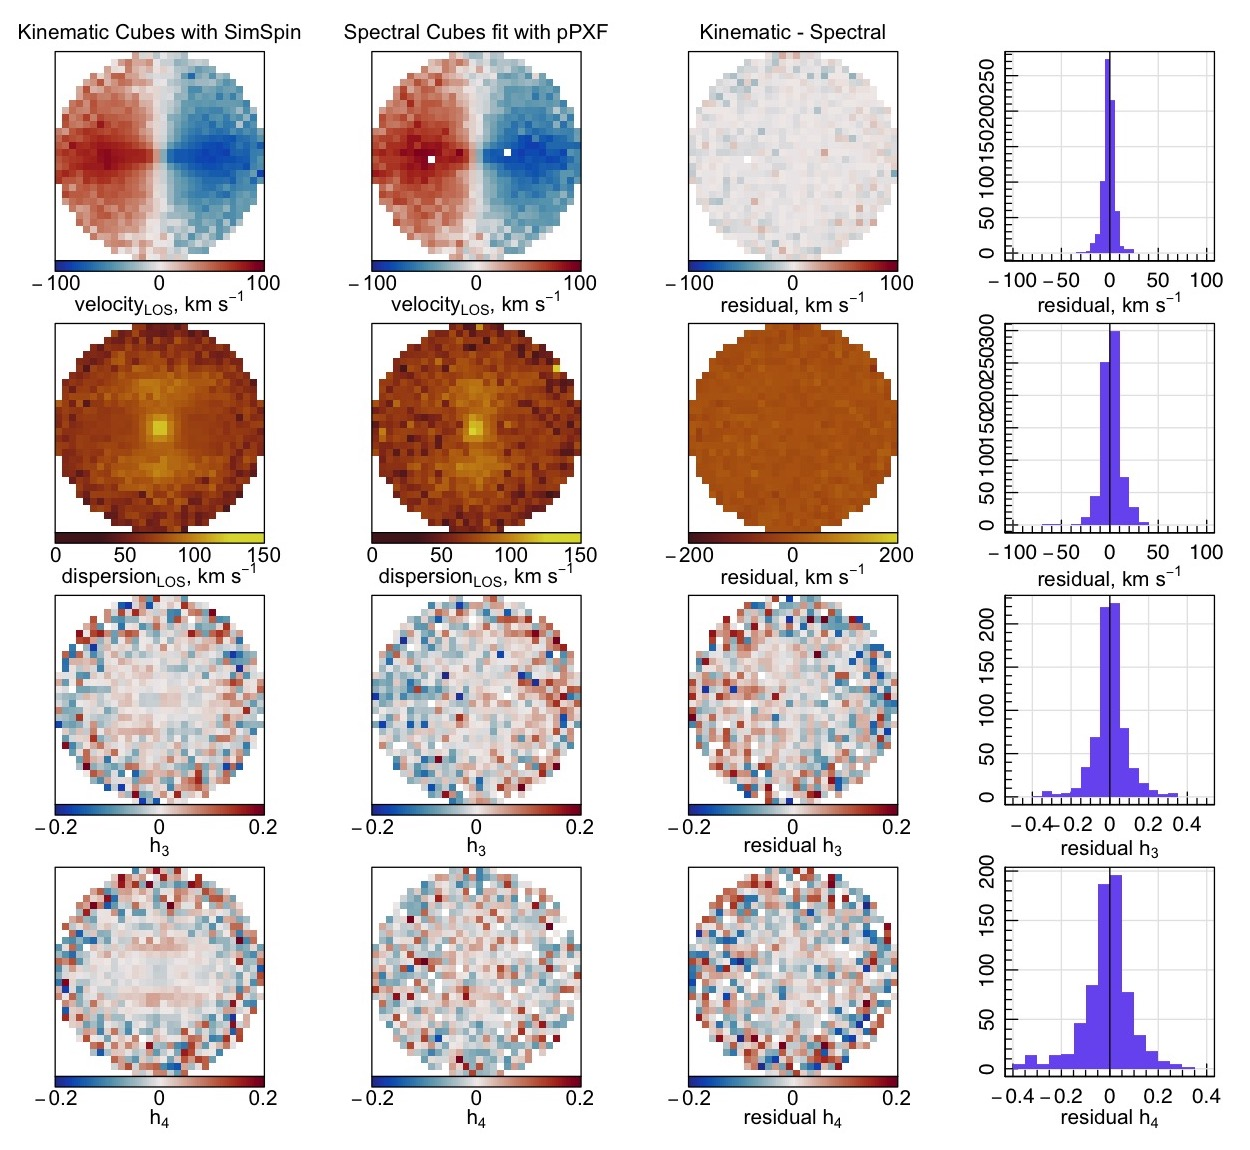
\includegraphics[keepaspectratio, width=8cm]{Figures/cs3_disk_velocities_highz_fwhm_EMILES.jpeg}
    \caption{Case Study 3: The disk model built with EMILES templates observed with an intrinsic telescope resolution of  $\lambda_{\text{LSF}}^{telescope} = 3.61$ \AA{} at a high redshift distance of $z = 0.3$. Here we compare the output kinematic cubes to the kinematics fit with pPXF.}
    \label{fig:cs3_disk_highz_EMILES}
\end{figure}

\begin{figure}
    \centering
    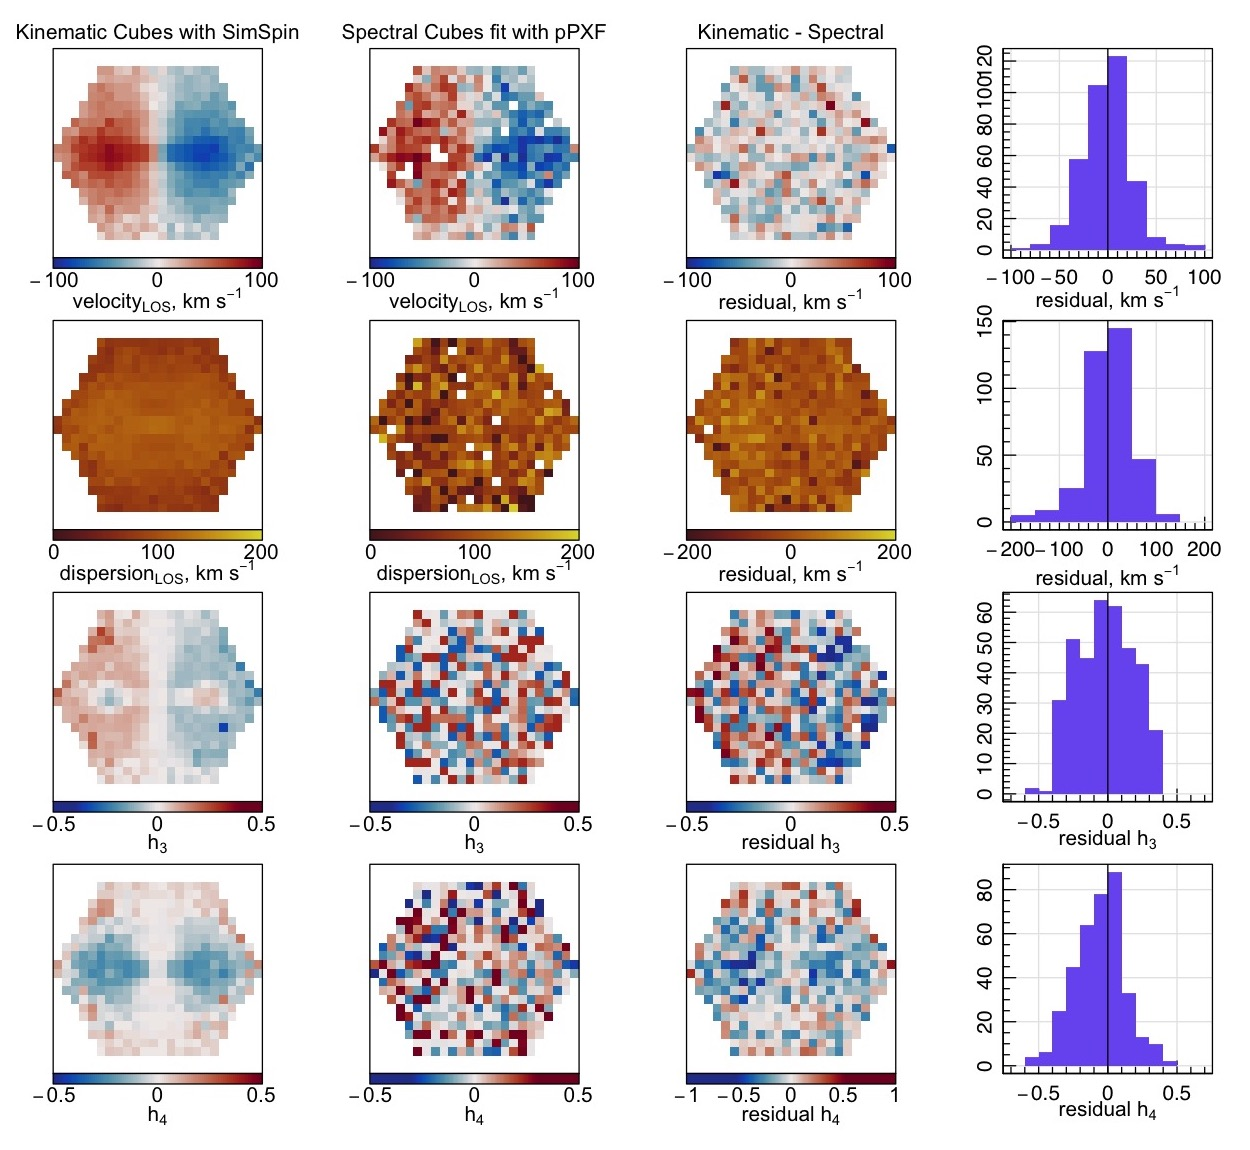
\includegraphics[keepaspectratio, width=8cm]{Figures/cs3_disk_velocities_highz_fwhm_BC03.jpeg}
    \caption{Case Study 3: The disk model built with BC03 templates observed with an intrinsic telescope resolution of  $\lambda_{\text{LSF}}^{telescope} = 4.56$ \AA{} at a high redshift distance of $z = 0.3$. Here we compare the output kinematic cubes to the kinematics fit with pPXF.}
    \label{fig:cs3_disk_highz_BC03}
\end{figure}

In Figure \ref{fig:cs3_disk_highz_EMILES}, we can see that the structure of the LOS dispersion has been well captured in the resulting spectral fit. 
However, we see that the higher order kinematics, $h_3$ and $h_4$ become quite difficult to explore as you go out in radius where noise begins to dominate.

We provide a direct comparison between the \textsc{GalexEV} and EMILES residuals in Figure \ref{fig:cs3_hist}, built at both high and low redshift.
It is quite clear from this comparison that there is no significant difference between the high and low redshift behaviour, except in the case of the cube built with \textsc{GalexEV} templates.
In this example, we see that the lower redshift model appears to under-estimate the true dispersion, as shown by the positive dispersion residuals. 

Given the difficulty we have had fitting the BC03 spectral models for kinematics, it is unclear whether these discrepancies are the fault of the \simspin{} code, or the fitting methodology. 
As the fits are quite consistent for the EMILES spectral cubes, we will proceed with the final test to check for consistency when atmospheric blurring conditions are incorporated. 

\begin{figure}
    \centering
    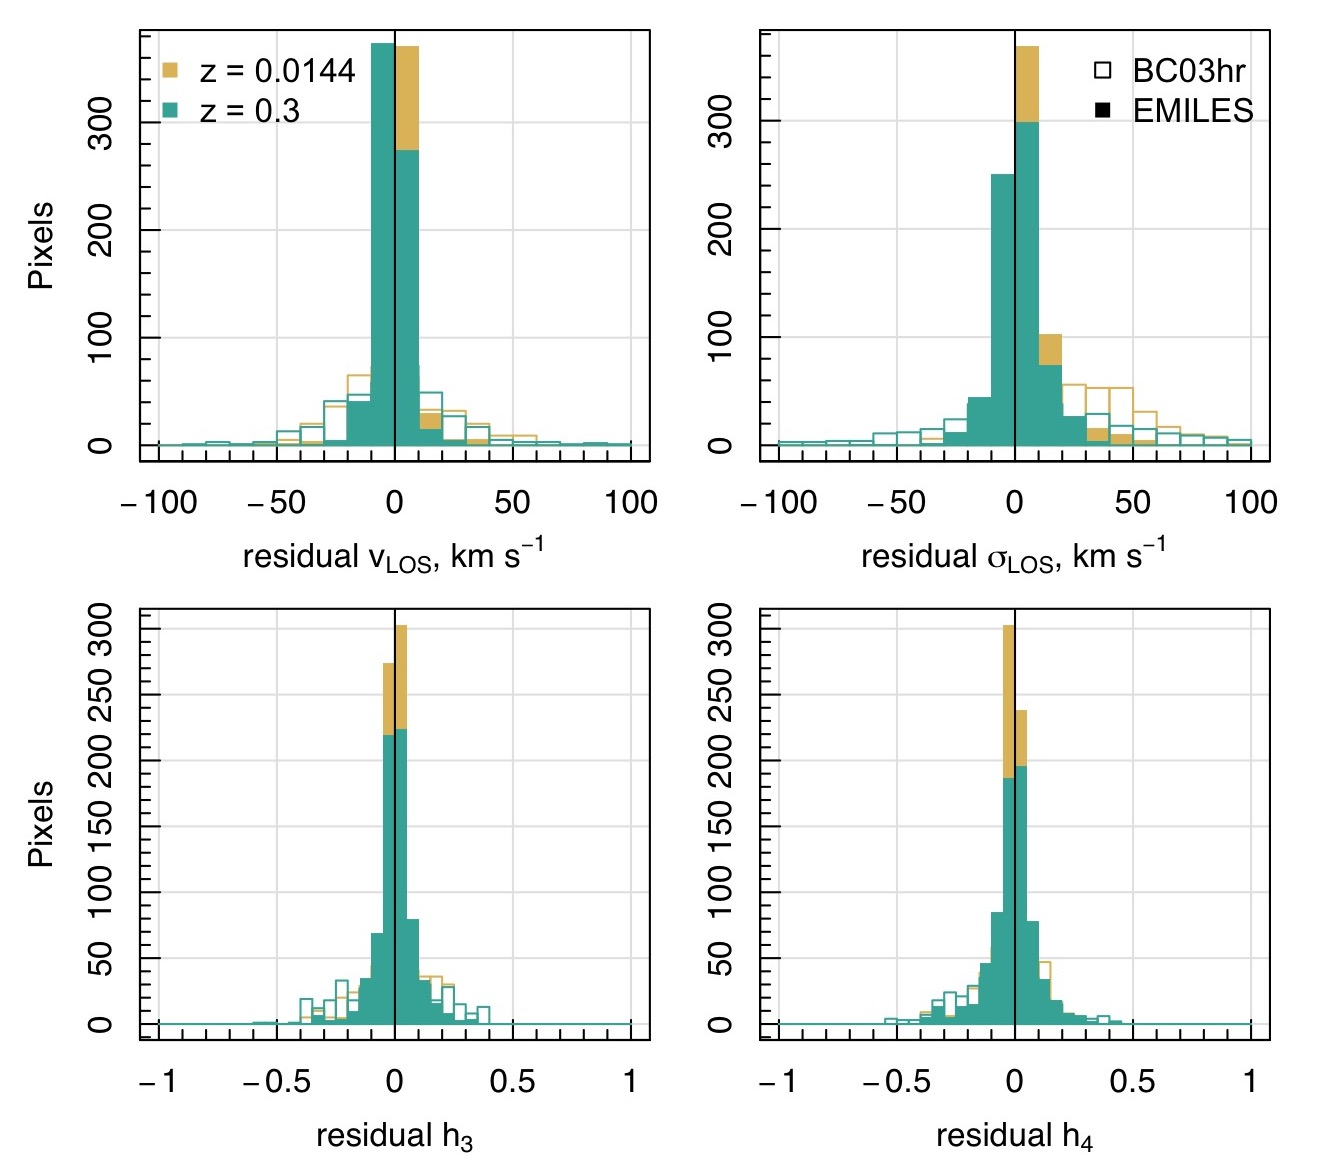
\includegraphics[keepaspectratio, width=8cm]{Figures/cs3_histograms.jpeg}
    \caption{Case Study 3: The residual differences between the kinematic observations and the spectral fits for the low and high redshift disc models (in yellow and green respectively) built with EMILES and BC03 templates. All distributions are nicely centred around zero as we would expect, though we do see significantly broader distributions for the BC03hr models in comparison to the EMILES models.}
    \label{fig:cs3_hist}
\end{figure}

\subsubsection*{Test 4: Observations with \telescope{} spectral resolution applied with atmospheric seeing conditions included. \\ }

The final test involves taking the previous mock observations, and introducing seeing conditions. 
As described in section \ref{sec:observation}, we convolve each spatial plane of our spectral or velocity data cube with a kernel to imitate the blurring effects of the atmosphere. 
This is done by specifying the \texttt{blur = T} parameter below, indicating that we would like the image to be blurred, as well as the size and shape of the convolution kernel. 
This is all done in the \observingstrategy{} function. 
For the following study, we use the following specification for the EMILES and \textsc{GalexEV} models, projecting each to both near and far distances with the varied seeing conditions:

\begin{lstlisting}[basicstyle=\fontsize{6}{8}\selectfont\ttfamily]
observing_strategy(dist_kpc_per_arcsec = 0.3, 
                   inc_deg = 60, blur = T,
                   fwhm = 1, 
                   psf="Gaussian")

observing_strategy(dist_z = 0.3, 
                   inc_deg = 60, blur = T,
                   fwhm = 2.8, 
                   psf="Moffat")
\end{lstlisting}

The rest of the \telescope{} parameters remain consistent with the previous case study. 
As in the previous case, we test these observations at both high and low redshift distances for the young disc model with the two flavours of spectral templates.
The results of these fits are demonstrated in Figures \ref{fig:cs4_disk_lowz_EMILES} and \ref{fig:cs4_disk_lowz_BC03}, where we show the fitting results for the low redshift EMILES galaxy and the high redshift BC03 galaxy. 
The remaining images are included in the final \ref{app:cs4}.

\begin{figure}
    \centering
    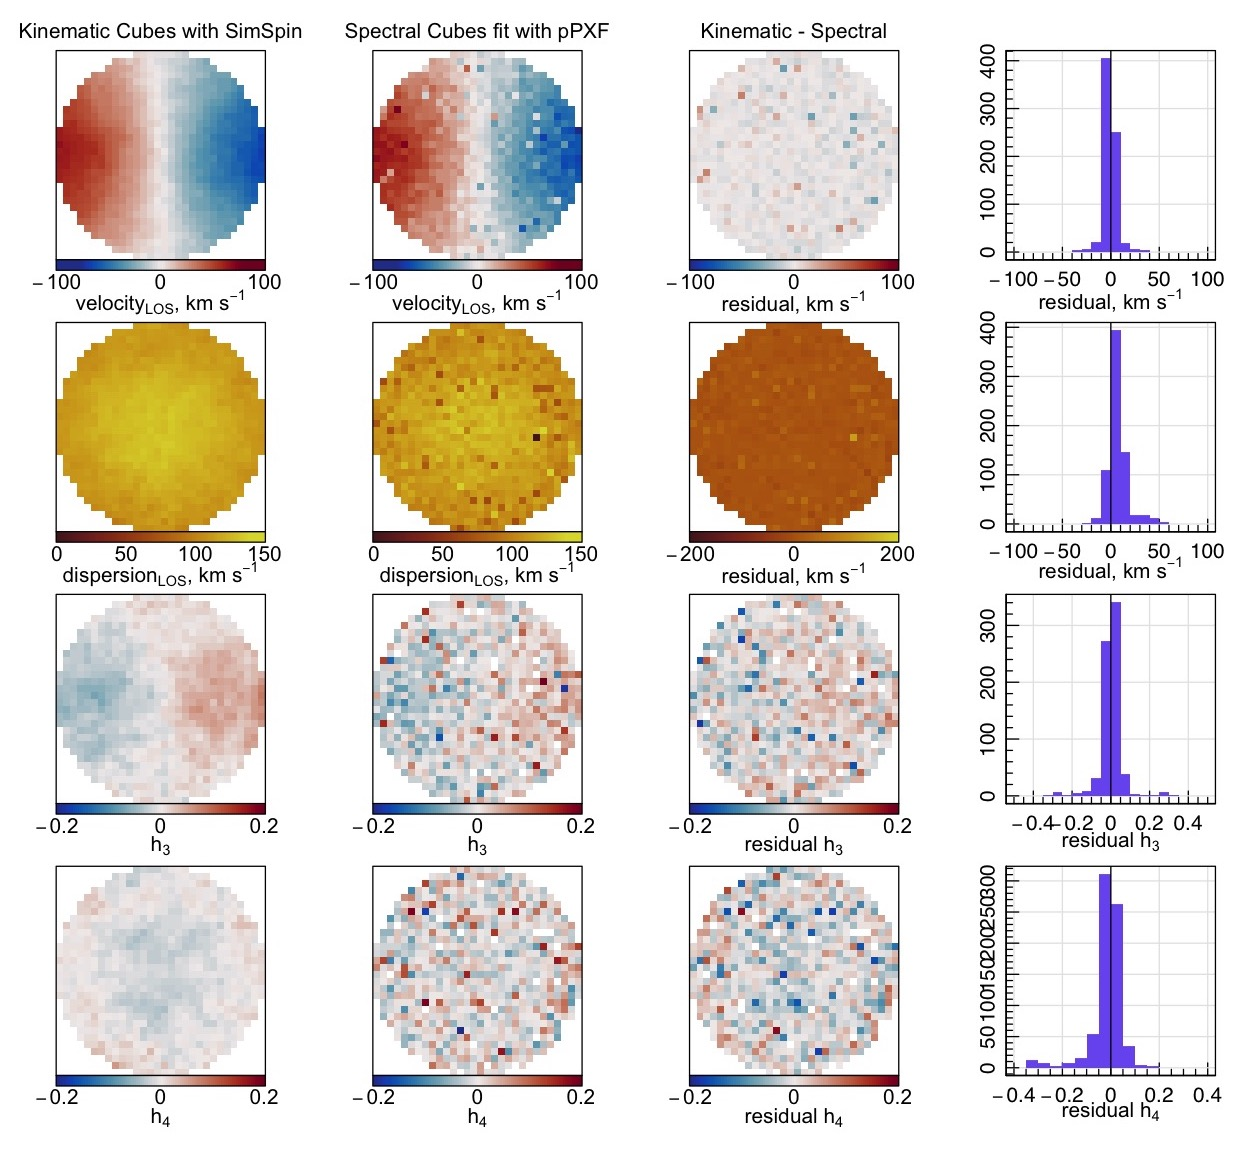
\includegraphics[keepaspectratio, width=8cm]{Figures/cs4_disk_velocities_lowz_fwhm_blur_EMILES.jpeg}
    \caption{Case Study 4: The disk model built with EMILES templates observed with an intrinsic telescope resolution of  $\lambda_{\text{LSF}}^{telescope} = 3.61$ \AA{} at a low redshift distance of $z = 0.0144$ with an added seeing condition of a Gaussian kernel with FWHM of 1 arcsec. Here we compare the output kinematic cubes to the kinematics fit with pPXF.}
    \label{fig:cs4_disk_lowz_EMILES}
\end{figure}

\begin{figure}
    \centering
    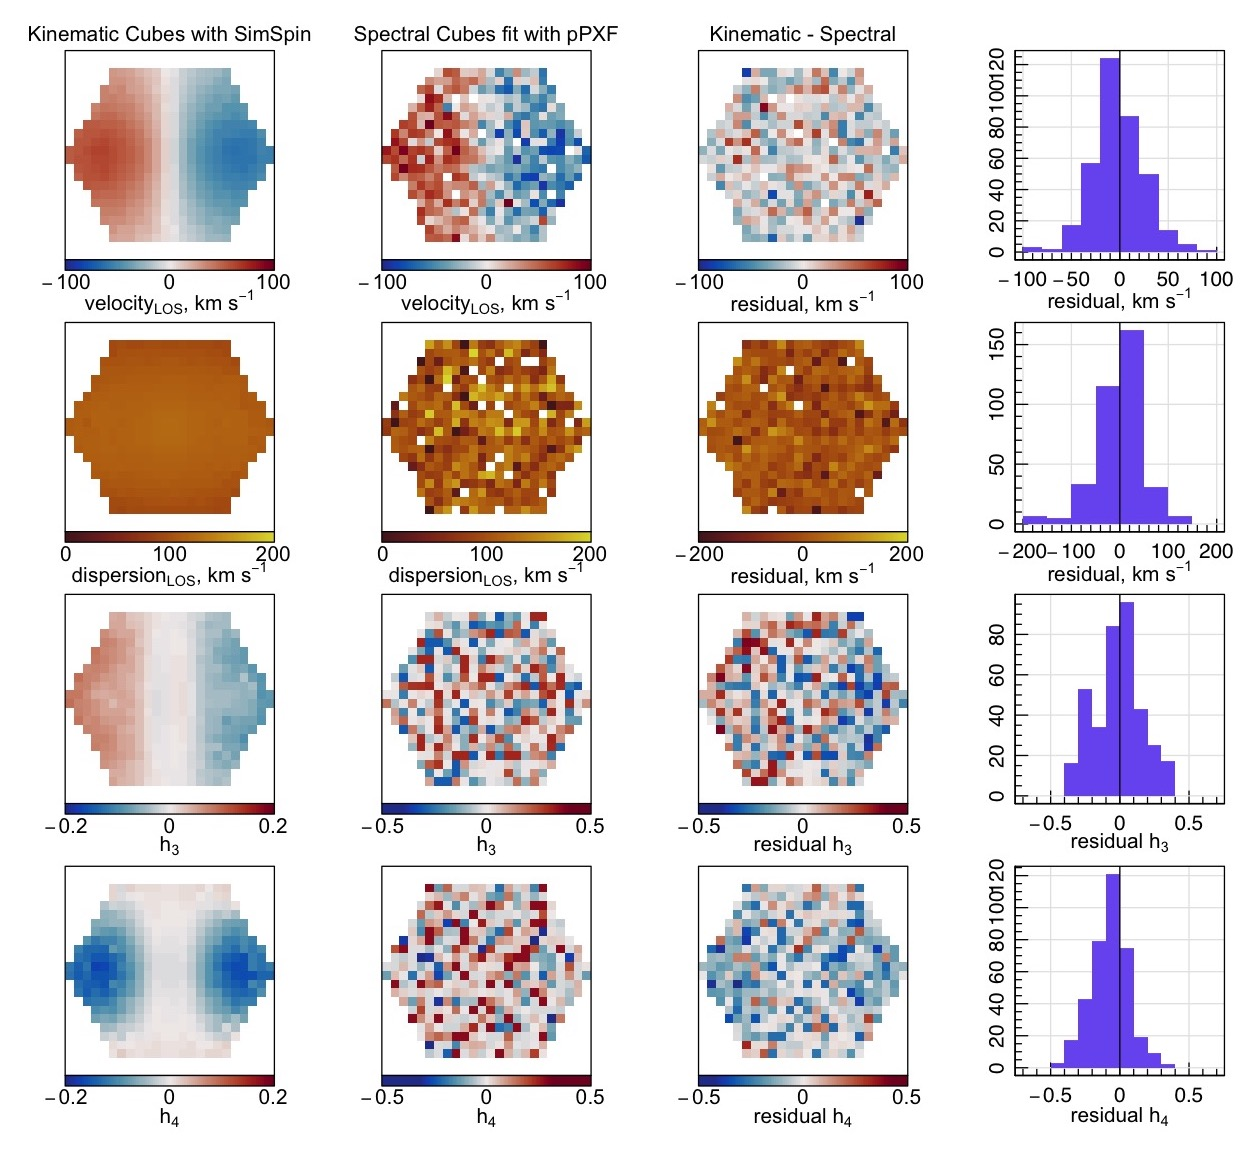
\includegraphics[keepaspectratio, width=8cm]{Figures/cs4_disk_velocities_highz_fwhm_blur_BC03.jpeg}
    \caption{Case Study 4: The disk model built with BC03 templates observed with an intrinsic telescope resolution of  $\lambda_{\text{LSF}}^{telescope} = 4.56$ \AA{} at a high redshift distance of $z = 0.3$ with an added seeing conditions of a Moffat kernel with FWHM of 2.8 arcsec. Here we compare the output kinematic cubes to the kinematics fit with pPXF.}
    \label{fig:cs4_disk_highz_BC03}
\end{figure}

Even in the blurred images, as shown in Figure \ref{fig:cs4_disk_lowz_EMILES}, we can see that the kinematics between the \texttt{method = "velocity"} and \texttt{"spectral"} cubes are closely comparable, with residuals nicely balanced around the zero point.
With the BC03 systems, we see a poorer recovery. 
Comparing the two directly using the histograms in Figure \ref{fig:cs4_hist}, a hollow yellow bump is visible towards the positive residuals showing that the kinematic cubes provide an overestimate of the dispersion in comparison to the spectral cube fit with pPXF. 

\begin{figure}
    \centering
    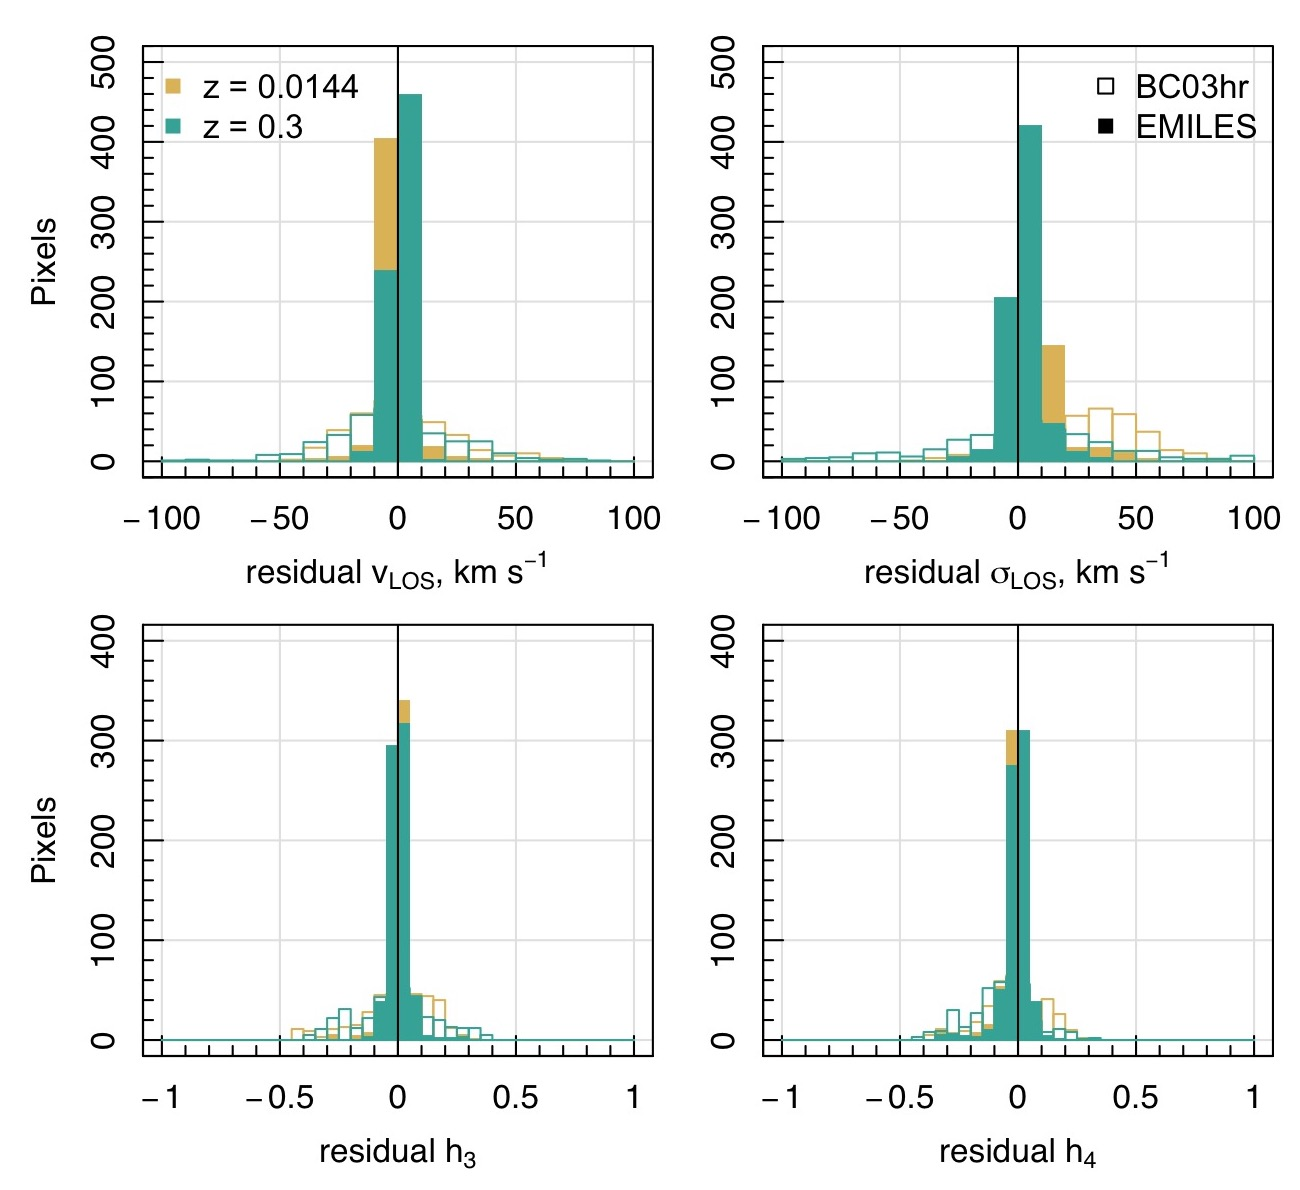
\includegraphics[keepaspectratio, width=8cm]{Figures/cs4_histograms.jpeg}
    \caption{Case Study 4: The residual differences between the kinematic observations and the spectral fits for the low and high redshift disc models (in yellow and green respectively) built with EMILES and BC03 templates. Most distributions are nicely centred around zero as we would expect, though we do see significantly broader distributions for the BC03hr models as well as some offset between the low redshift dispersion measured.}
    \label{fig:cs4_hist}
\end{figure}

\vspace{0.5cm}

These are important tests to run in order to evaluate the success and flexibility of the code. 
Here we have taken each feature in turn and assessed how it's addition affects the resulting kinematic image. 
We note that, within the extra-galactic community, the use of EMILES templates for kinematic fitting is commonplace and as such it is good to see the consistency between input and output in the simulations that have been built and kinematics fit using the same set of stellar population synthesis models. 
Concern is raised with regards to the poorer fits found between the BC03 models fit using EMILES templates. 
The \textsc{GalexEV} empirical templates are empirical evolutionary stellar population synthesis codes that are commonly used within the theory community for semi-analytic models and for stellar population fitting. 

\vspace{0.5cm}

\subsection{Web application}
\simspin{} is a flexible and modular code, as demonstrated in this article and the numerous examples available online. 
As the number of applications for mock simulation data grows with ever more resolved models of galaxy formation and evolution, it is important that access to the code is accessible and usable by a wide range of users, theorists and observers alike.
In order to remove some of the barriers we perceive preventing users working with this code (including working with \small{R}, handling simulation data, or running large memory jobs locally), we have built a web application of \simspin  \footnote{\url{https://simspin.datacentral.org.au/app/}}. 

The \simspin{} web application has the same range of functionality as the R-package, without the necessity to download and install the package yourself.
It is a performant React Single Page App communicating asynchronously with a RESTful API, hosted by Data Central. 
The application allows for instant data exploration via a dedicated viewer, where authenticated users can re-visit previous queries and share results with others. 
Generated FITS files can be directly downloaded for further exploration and quantification. 
All services are containerised and managed by docker compose, such that the project is easily re-deployable. 
The API is fully documented, and comes with an API Schema (adhering to the OpenAPI Specification) to aid users in calling the API from other services.

The SimSpin app removes the barrier of entry for novice astronomers, providing an accessible and time-saving tool for simulated galaxy visualisations.
The API further removes a code language barrier as individuals can generate \simspin{} queries using whichever language they choose. 
An example of this can be found within the documentation.\footnote{\url{https://kateharborne.github.io/SimSpin/examples/query_the_API.html}}.

\section{CONCLUSION}

In conclusion, we have presented a significant update to the mock observation code, \simspin. 
We have demonstrated a number of new features available in the code \ssversion, including the measurement of higher-order kinematics, the construction of spectral data cubes and the inclusion of gas component analysis.
The code now supports a wide number of different hydrodynamical simulations, including \eagle, \illustristng, \magneticum, and \horizon. 
We further have containerised the code into a web application such that anyone can work with mock data, regardless of their coding language or computer specifications. 

All of these features have been tested using unit testing, as well as the longer case study explorations that are presented in the results of this paper. 
In line with standard continuous integration procedures, we run all unit tests and require them to pass before any changes can be merged into the main branch of the code. 
We also require the code coverage (as measured by the number of lines within the code hit by the unit tests) to remain at approximately 90\% for tests to pass. 
In the future, as more developers aim to expand the capabilities of the code, we may further implement another set of checks by core developers using the review system in place through GitHub. 

The range of applications for this code is already beginning to be demonstrated within the literature for applications from designing corrections for the effects of seeing conditions \citep{Harborne2020RecoveringData}, exploring the observational signatures of slow rotating systems formed in different ways \citep{Lagos2022Thesimulations}, or building machine learning models to explore the connection between intrinsic 3D shape and observable kinematics (Yong et al., in prep). 
Of particular interest, with the ready incorporation of theory data with observational surveys, we hope to see similar data releases of simulated galaxies for comparison alongside observations  \citep[such as is being prepared for the MAGPI survey as described in][]{Foster2021MAGPIOverview}. 
With tools like \simspin, we are enabling these comparisons to be made consistently, both between simulations and observations, but also consistently between the different simulations themselves. 

Simulations provide us with the ability to explore the far reaches of space and time, while \simspin{} now enables us to compare these simulations to our exquisite observations. 
The benefit of this is that, we our models we know the ground truth - projection effects can be modified by simply moving our observer, the atmosphere can be turned "on" or "off", and we can fast-forward through time to examine how a given system may change over the course of it's life. 
Such information is undoubtedly useful for contextualising the results we find in observations, as well as to improve existing sub-grid recipes within simulations in line with this. 
The future of mock observables is bright. 



\bibliography{references}


\appendix

%\section{The importance of de-redshifting spectra at low $z$}
%\label{app:rest}

%Throughout our case studies presented in section \ref{sec:cs1}, we used pPXF to fit our spectral cubes for comparison with the kinematic measurements.
%During this exercise, we had a number of different co-authors running the fits using their own implementations of the code in order to understand the robustness of our results. 

%It was of interest that, despite the comments within the examples within the code, we found a significant change in predicted dispersion measures when choosing to return low-redshift observations to the rest-frame. 
%We show the results of the two methods here.
%Both fits appear reasonable but we note the difference between the two dispersion maps output by the code. 

%As we can compare these results with the intrinsic kinematics of the underlying simulation, we can tell that the `more correct` methodology is to return any spectrum to the rest-frame before fitting the kinematics. 

%We demonstrate this in \ref{fig:}

\section{Additional case study figures}
\subsection{Observations of intrinsic template spectral resolution at low redshift}
\label{app:cs1}

Here, in Figures \ref{fig:cs1_bulge_EMILES}-\ref{fig:cs1_oldbulge_BC03}, we present the young bulge and old bulge observations from case study 1, where we have used the intrinsic spectral resolution of the underlying templates at a negligible redshift of $z = 0.0144$. The hexagonal maps are those models that have been built with the BC03 templates, while the circular maps have been built with the EMILES templates. 

\begin{figure}
    \centering
    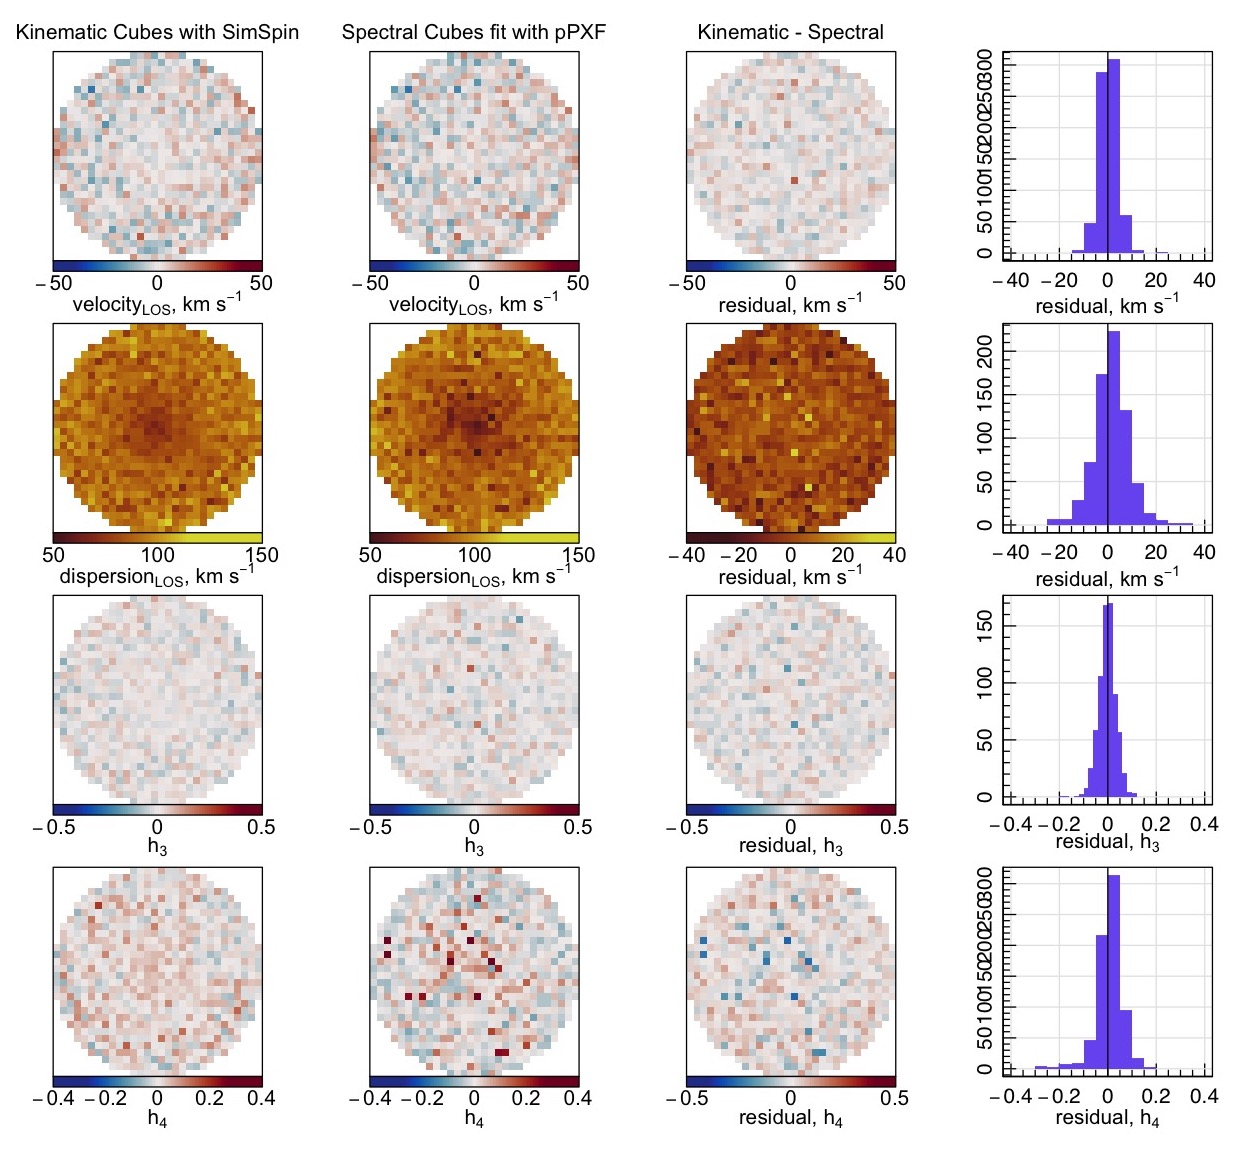
\includegraphics[keepaspectratio, width=8cm]{Figures/cs1_bulge_velocities_lowz_EMILES.jpeg}
    \caption{Case Study 1: The bulge model built with EMILES templates observed with an intrinsic telescope resolution of  $\lambda_{\text{LSF}}^{telescope} = 0$ \AA{} at a low redshift distance of $z = 0.0144$. Here we compare the output kinematic cubes to the kinematics fit with pPXF.}
    \label{fig:cs1_bulge_EMILES}
\end{figure}

\begin{figure}
    \centering
    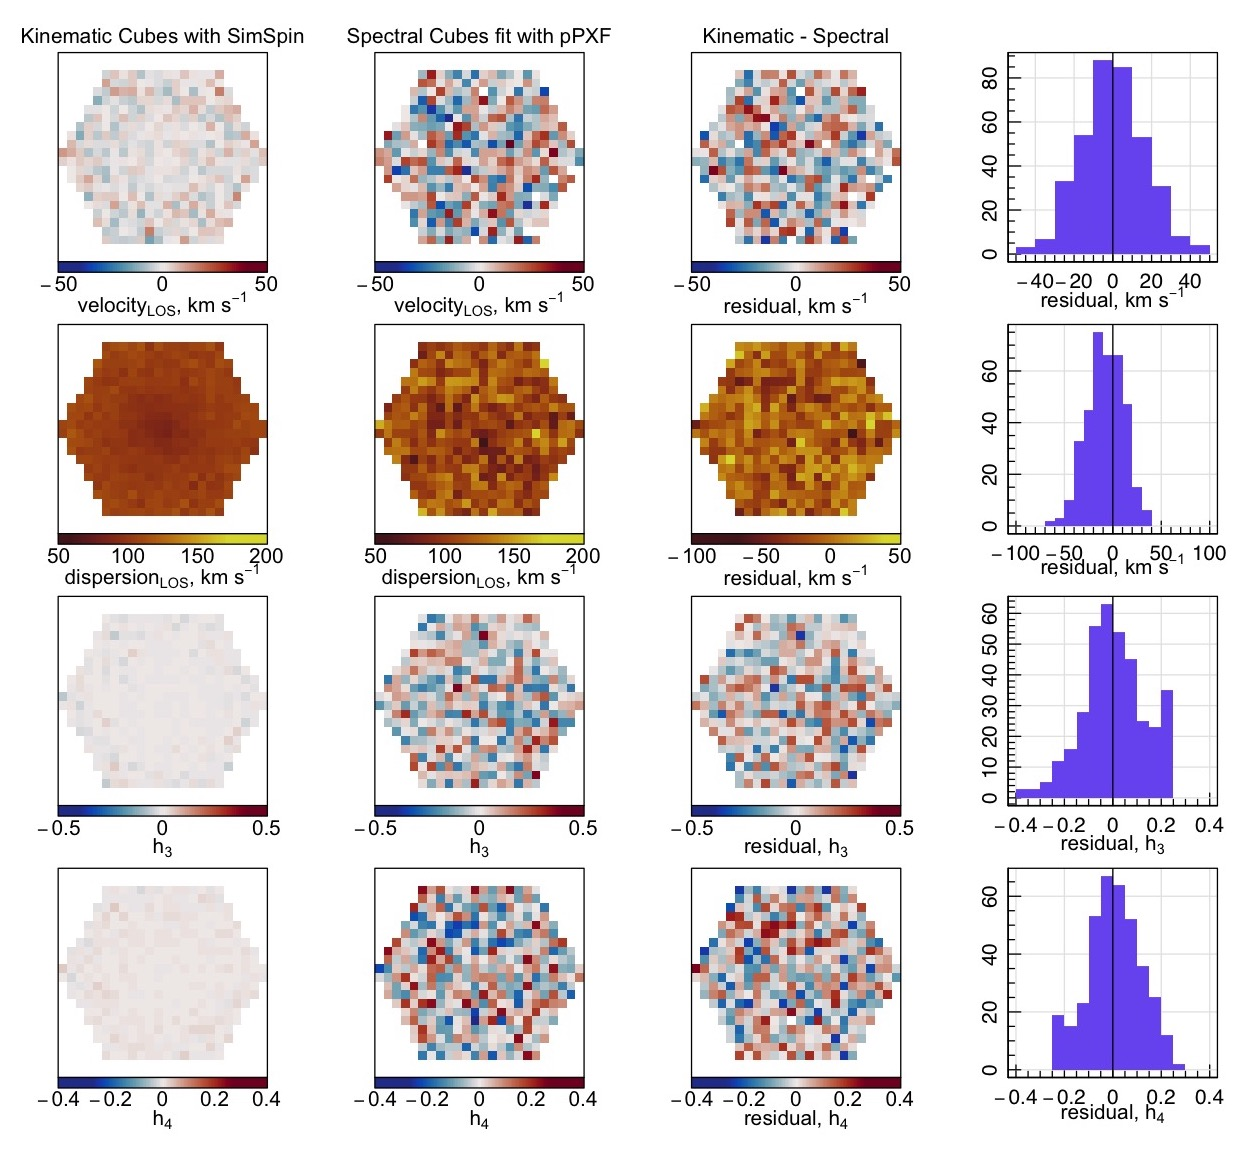
\includegraphics[keepaspectratio, width=8cm]{Figures/cs1_bulge_velocities_lowz_BC03hr.jpeg}
    \caption{Case Study 1: The bulge model built with BC03 templates observed with an intrinsic telescope resolution of  $\lambda_{\text{LSF}}^{telescope} = 0$ \AA{} at a low redshift distance of $z = 0.0144$. Here we compare the output kinematic cubes to the kinematics fit with pPXF.}
    \label{fig:cs1_bulge_BC03}
\end{figure}

\begin{figure}
    \centering
    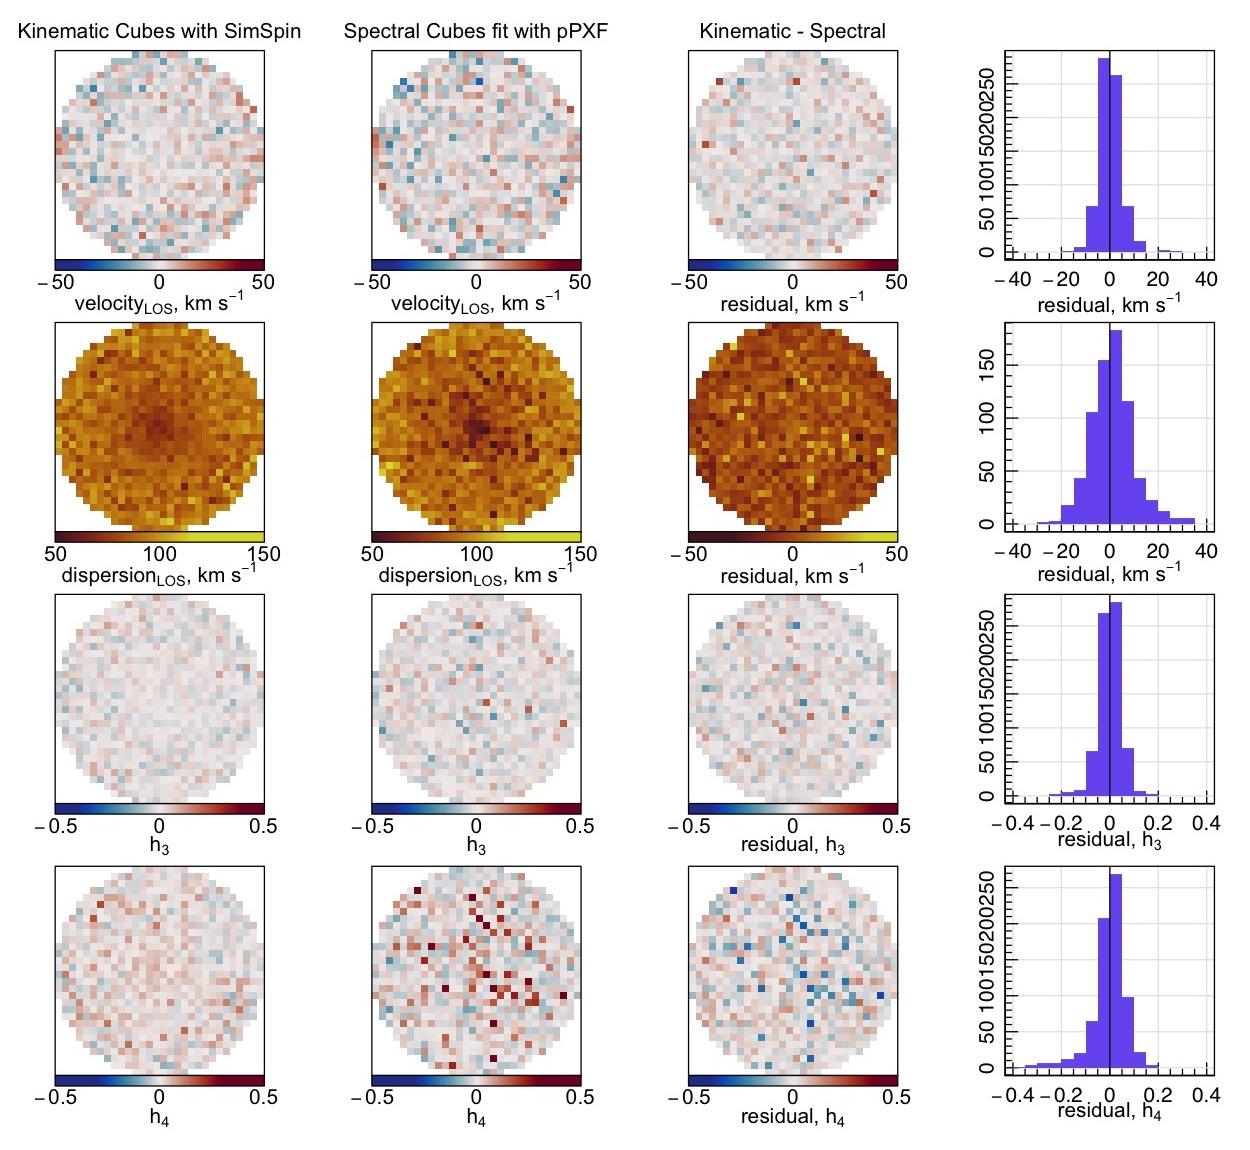
\includegraphics[keepaspectratio, width=8cm]{Figures/cs1_old_bulge_velocities_lowz_EMILES.jpeg}
    \caption{Case Study 1: The old bulge model built with EMILES templates observed with an intrinsic telescope resolution of  $\lambda_{\text{LSF}}^{telescope} = 0$ \AA{} at a low redshift distance of $z = 0.0144$. Here we compare the output kinematic cubes to the kinematics fit with pPXF.}
    \label{fig:cs1_oldbulge_EMILES}
\end{figure}

\begin{figure}
    \centering
    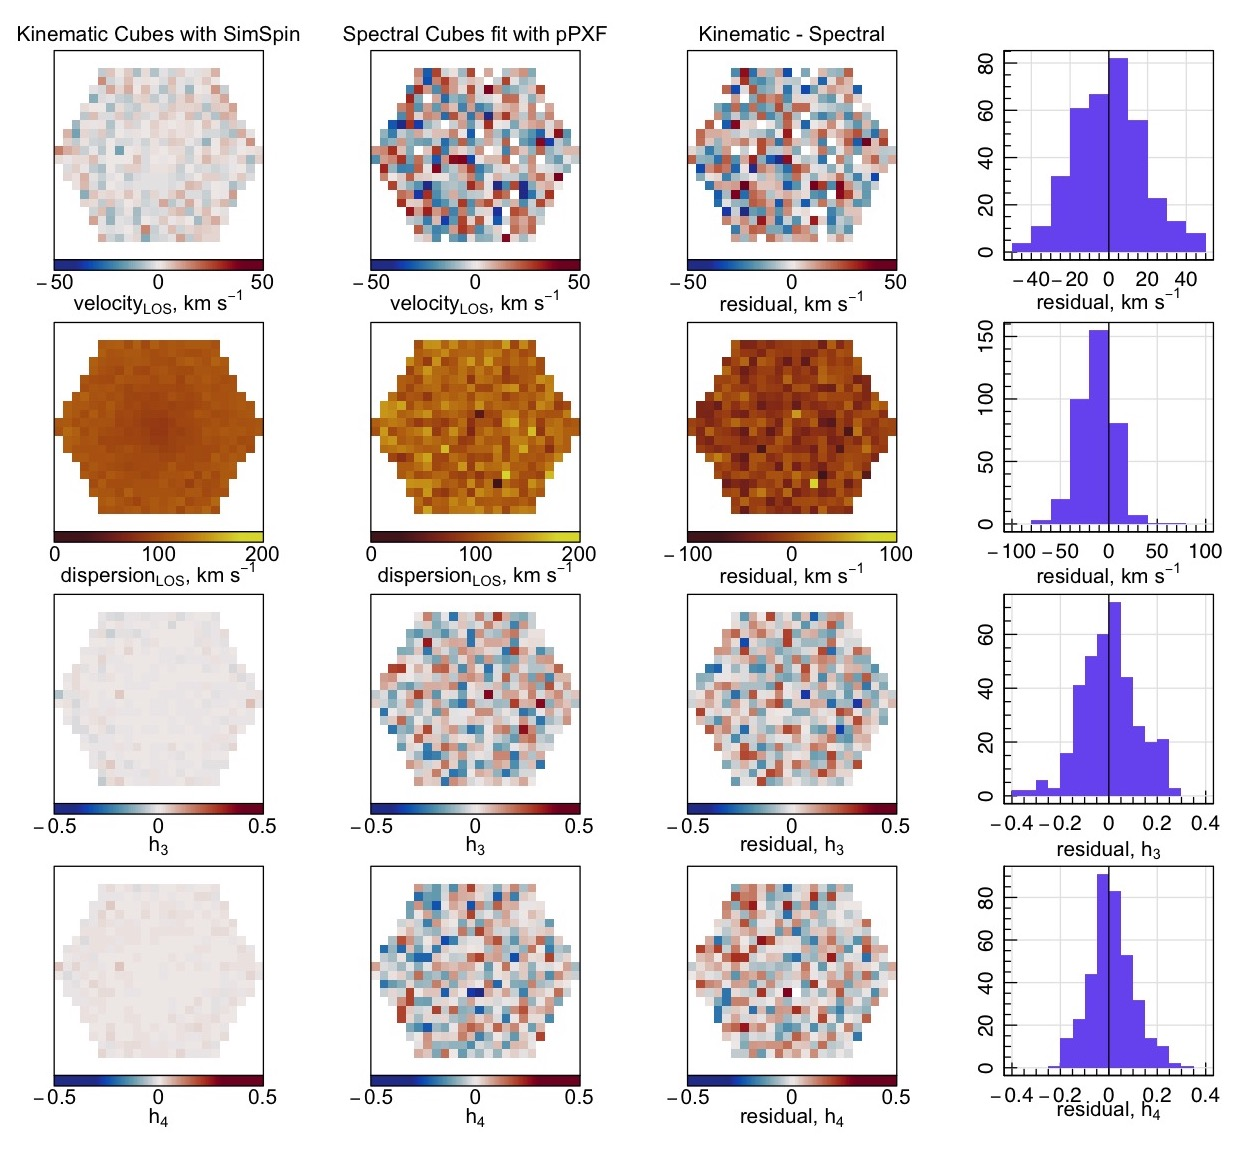
\includegraphics[keepaspectratio, width=8cm]{Figures/cs1_old_bulge_velocities_lowz_BC03hr.jpeg}
    \caption{Case Study 1: The old bulge model built with BC03 templates observed with an intrinsic telescope resolution of  $\lambda_{\text{LSF}}^{telescope} = 0$ \AA{} at a low redshift distance of $z = 0.0144$. Here we compare the output kinematic cubes to the kinematics fit with pPXF.}
    \label{fig:cs1_oldbulge_BC03}
\end{figure}

\FloatBarrier

\subsection{Observations of intrinsic template spectral resolution at high redshift}
\label{app:cs2}

Here, in Figures \ref{fig:cs2_disk_EMILES}-\ref{fig:cs2_oldbulge_BC03}, we present the young disc and old bulge observations from case study 2, where we have used the intrinsic spectral resolution of the underlying templates shifted up to a redshift of $z = 0.3$. The hexagonal maps are those models that have been built with the BC03 templates, while the circular maps have been built with the EMILES templates. 

\begin{figure}
    \centering
    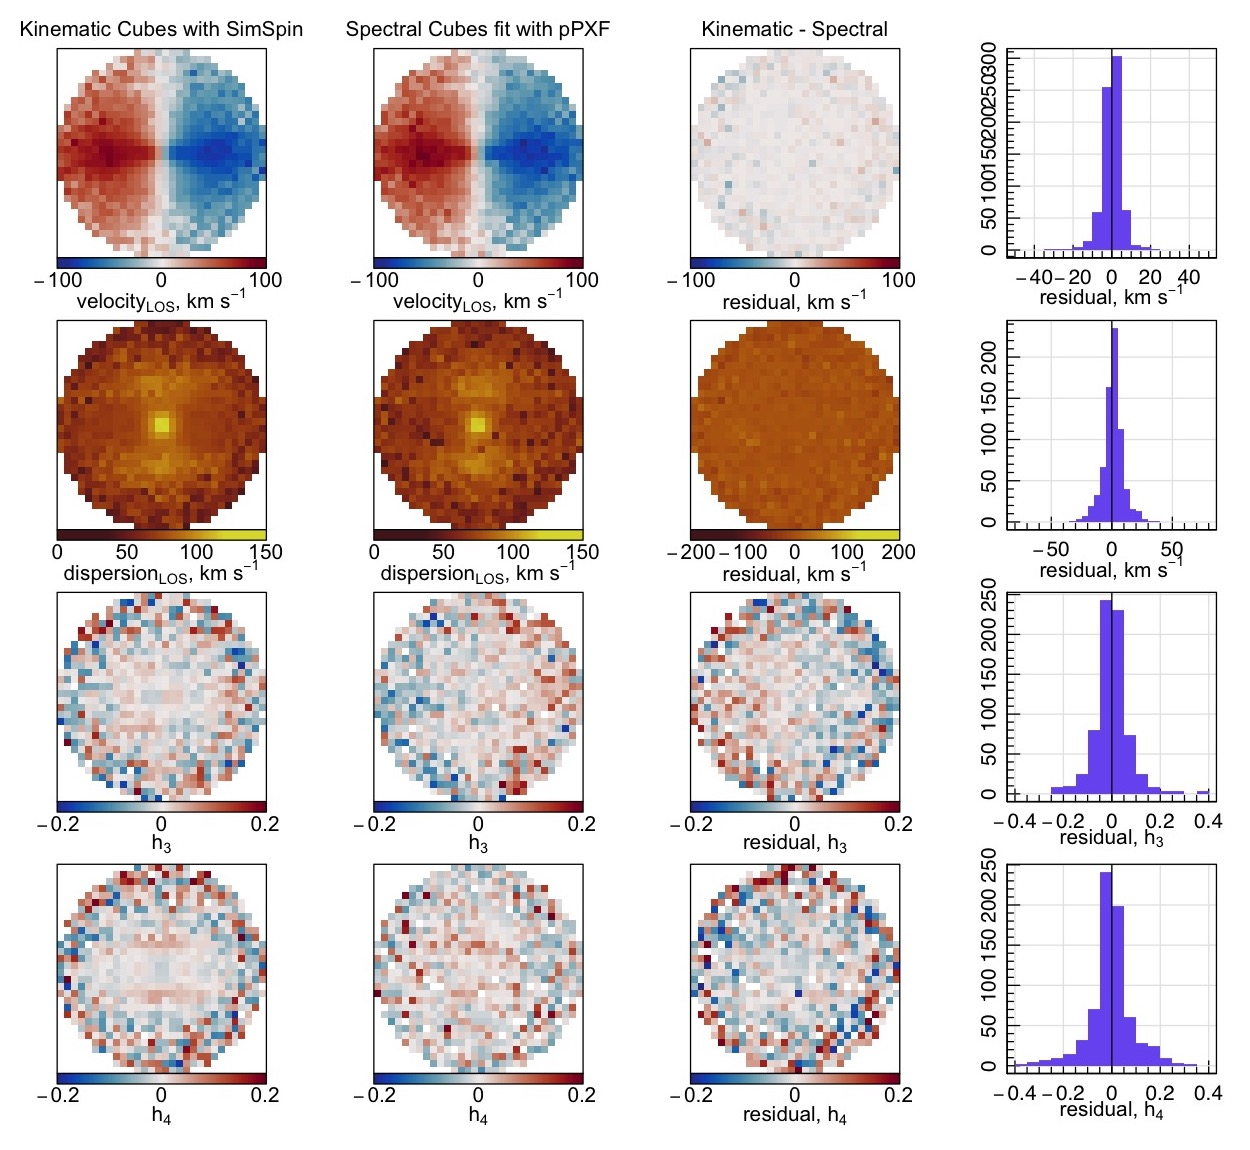
\includegraphics[keepaspectratio, width=8cm]{Figures/cs2_disk_velocities_highz_EMILES.jpeg}
    \caption{Case Study 2: The disk model built with EMILES templates observed with an intrinsic telescope resolution of  $\lambda_{\text{LSF}}^{telescope} = 0$ \AA{} at a high redshift distance of $z = 0.3$. Here we compare the output kinematic cubes to the kinematics fit with pPXF.}
    \label{fig:cs2_disk_EMILES}
\end{figure}

\begin{figure}
    \centering
    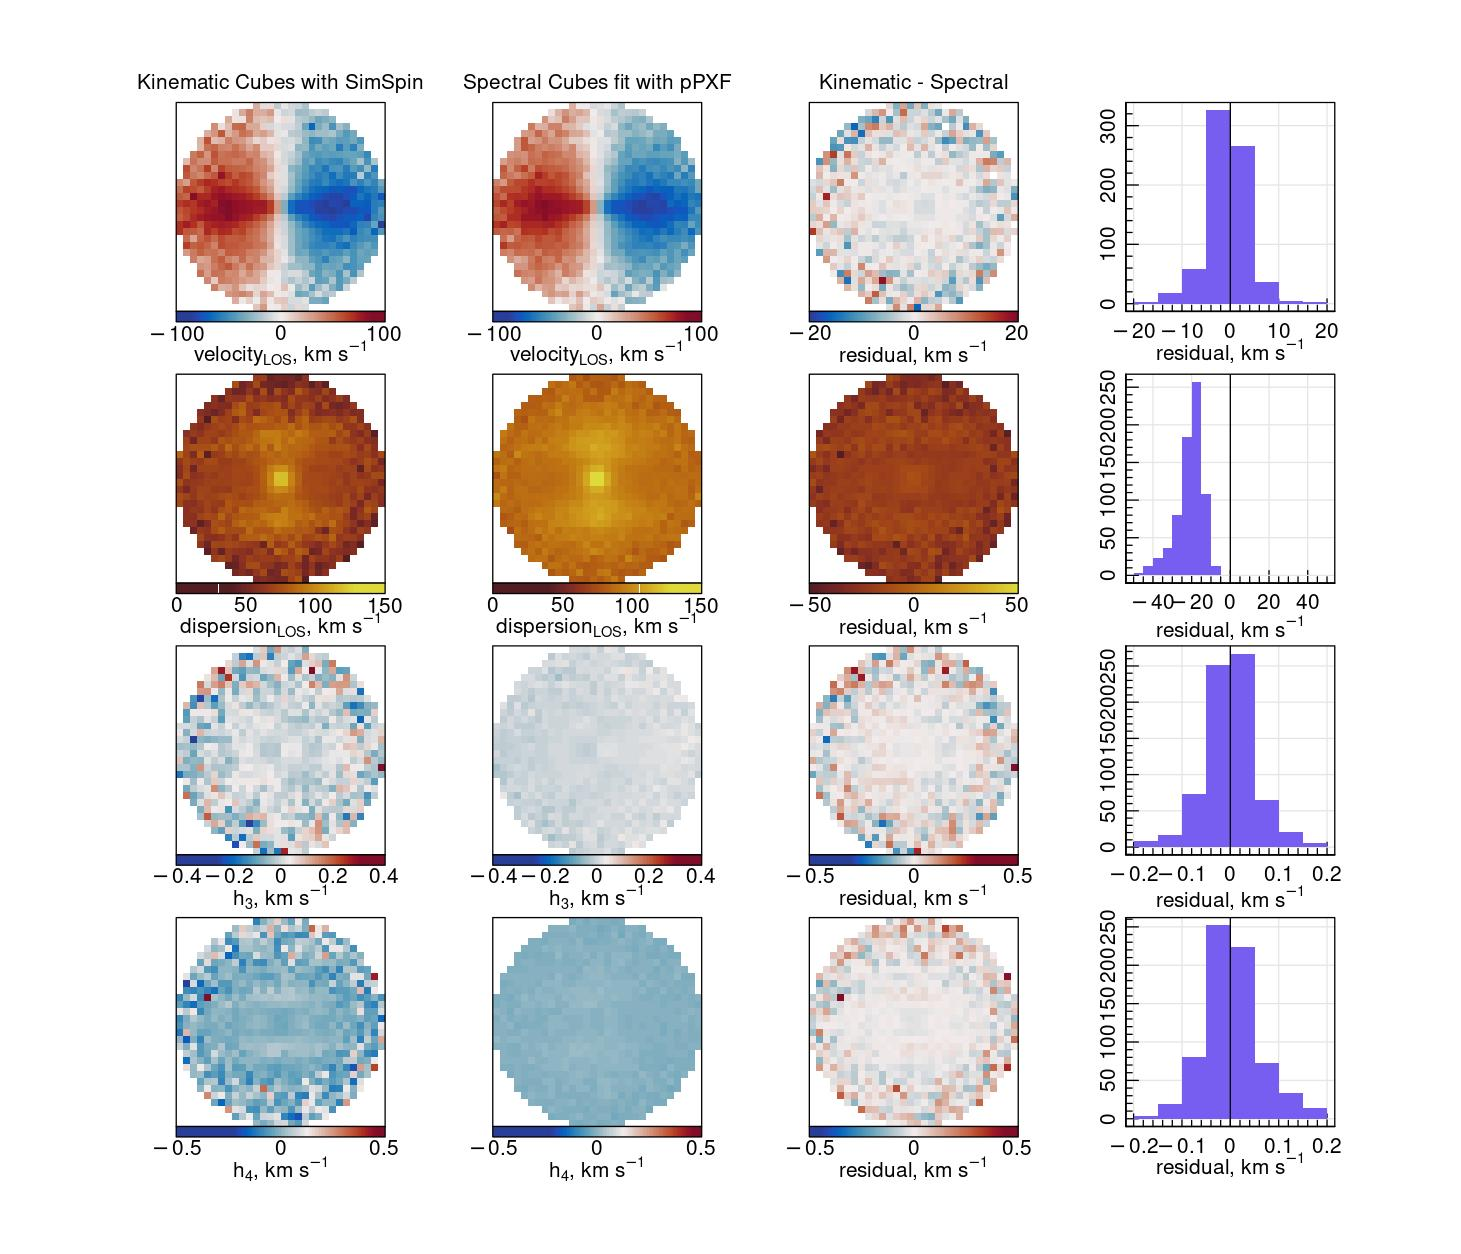
\includegraphics[keepaspectratio, width=8cm]{Figures/cs2_disk_velocities_highz_BC03hr.jpeg}
    \caption{Case Study 2: The disk model built with BC03 templates observed with an intrinsic telescope resolution of  $\lambda_{\text{LSF}}^{telescope} = 0$ \AA{} at a high redshift distance of $z = 0.3$. Here we compare the output kinematic cubes to the kinematics fit with pPXF.}
    \label{fig:cs2_disk_BC03}
\end{figure}

\begin{figure}
    \centering
    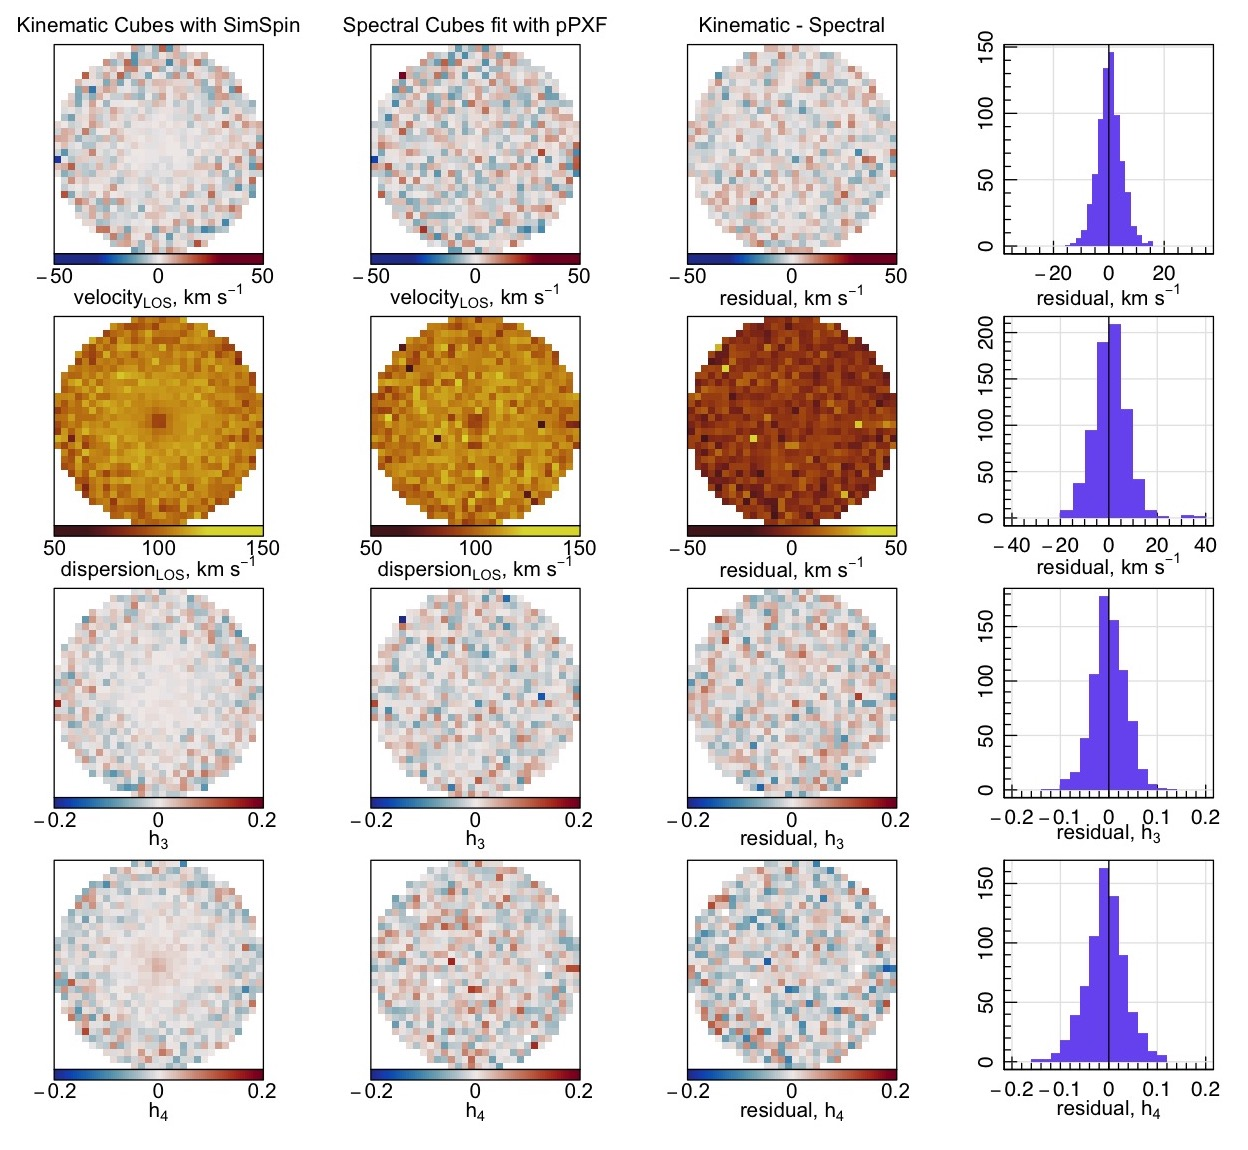
\includegraphics[keepaspectratio, width=8cm]{Figures/cs2_old_bulge_velocities_highz_EMILES.jpeg}
    \caption{Case Study 2: The old bulge model built with EMILES templates observed with an intrinsic telescope resolution of  $\lambda_{\text{LSF}}^{telescope} = 0$ \AA{} at a high redshift distance of $z = 0.3$. Here we compare the output kinematic cubes to the kinematics fit with pPXF.}
    \label{fig:cs2_oldbulge_EMILES}
\end{figure}

\begin{figure}
    \centering
    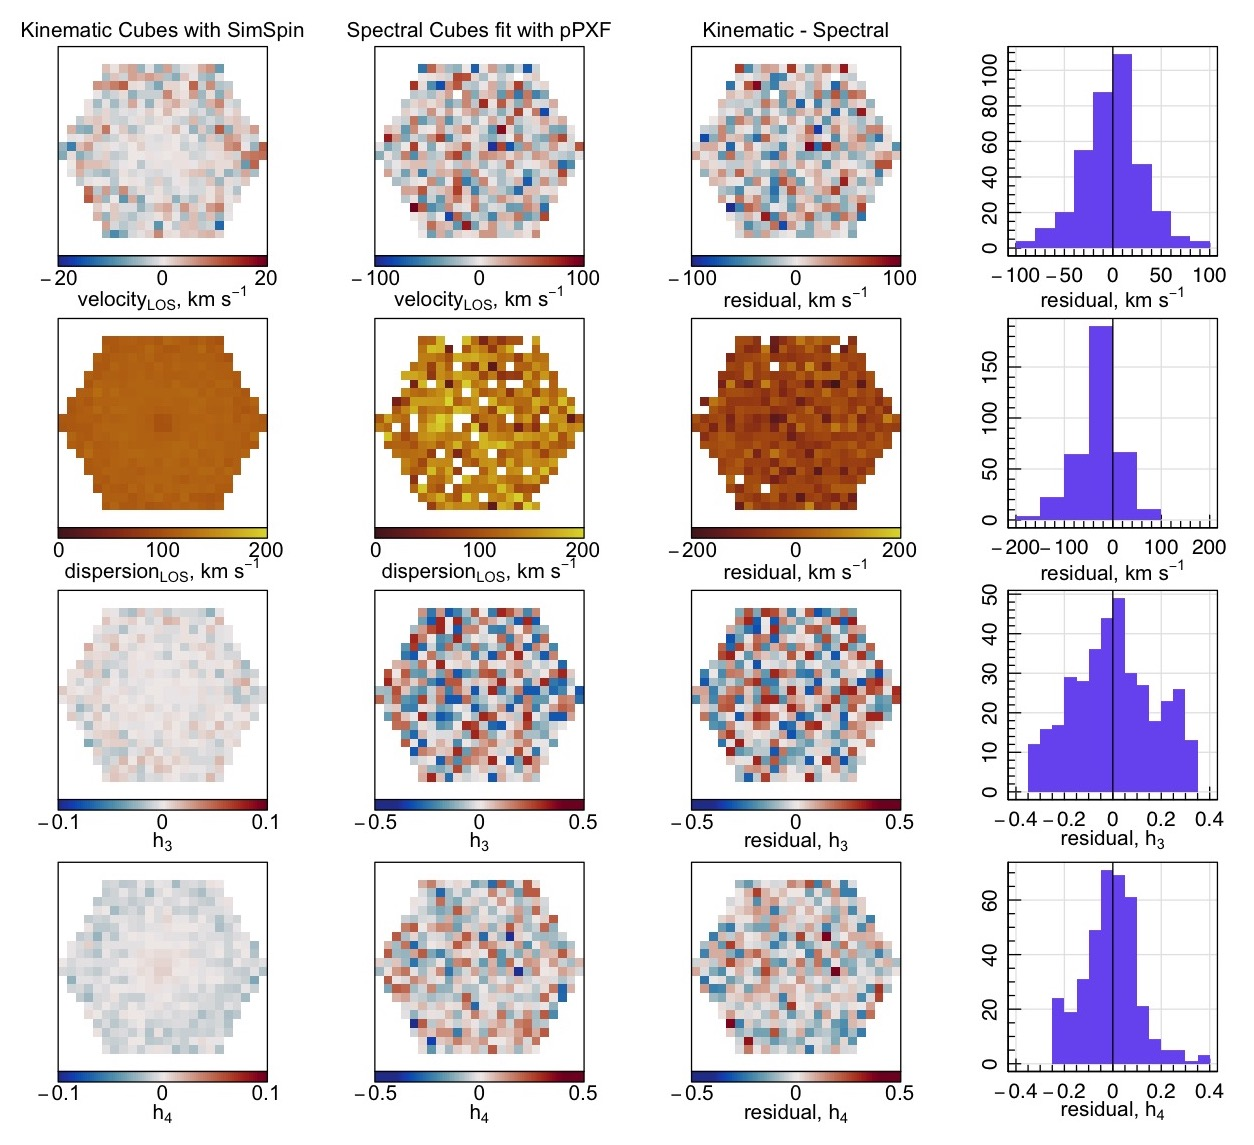
\includegraphics[keepaspectratio, width=8cm]{Figures/cs2_old_bulge_velocities_highz_BC03hr.jpeg}
    \caption{Case Study 2: The old bulge model built with BC03 templates observed with an intrinsic telescope resolution of  $\lambda_{\text{LSF}}^{telescope} = 0$ \AA{} at a high redshift distance of $z = 0.3$. Here we compare the output kinematic cubes to the kinematics fit with pPXF.}
    \label{fig:cs2_oldbulge_BC03}
\end{figure}

\FloatBarrier

\subsection{Observations of with \telescope{} spectral resolution at low \& high redshift}
\label{app:cs3}

Here, in Figures \ref{fig:cs3_disk_lowz_EMILES}-\ref{fig:cs3_disk_lowz_BC03}, we present the young disc low-$z$ observations from case study 3, where we have used \telescope{} spectral resolutions of 3.61\AA{} and 4.56\AA{} for the EMILES and BC03 models respectively. The hexagonal maps are those models that have been built with the BC03 templates, while the circular maps have been built with the EMILES templates. 

\begin{figure}
    \centering
    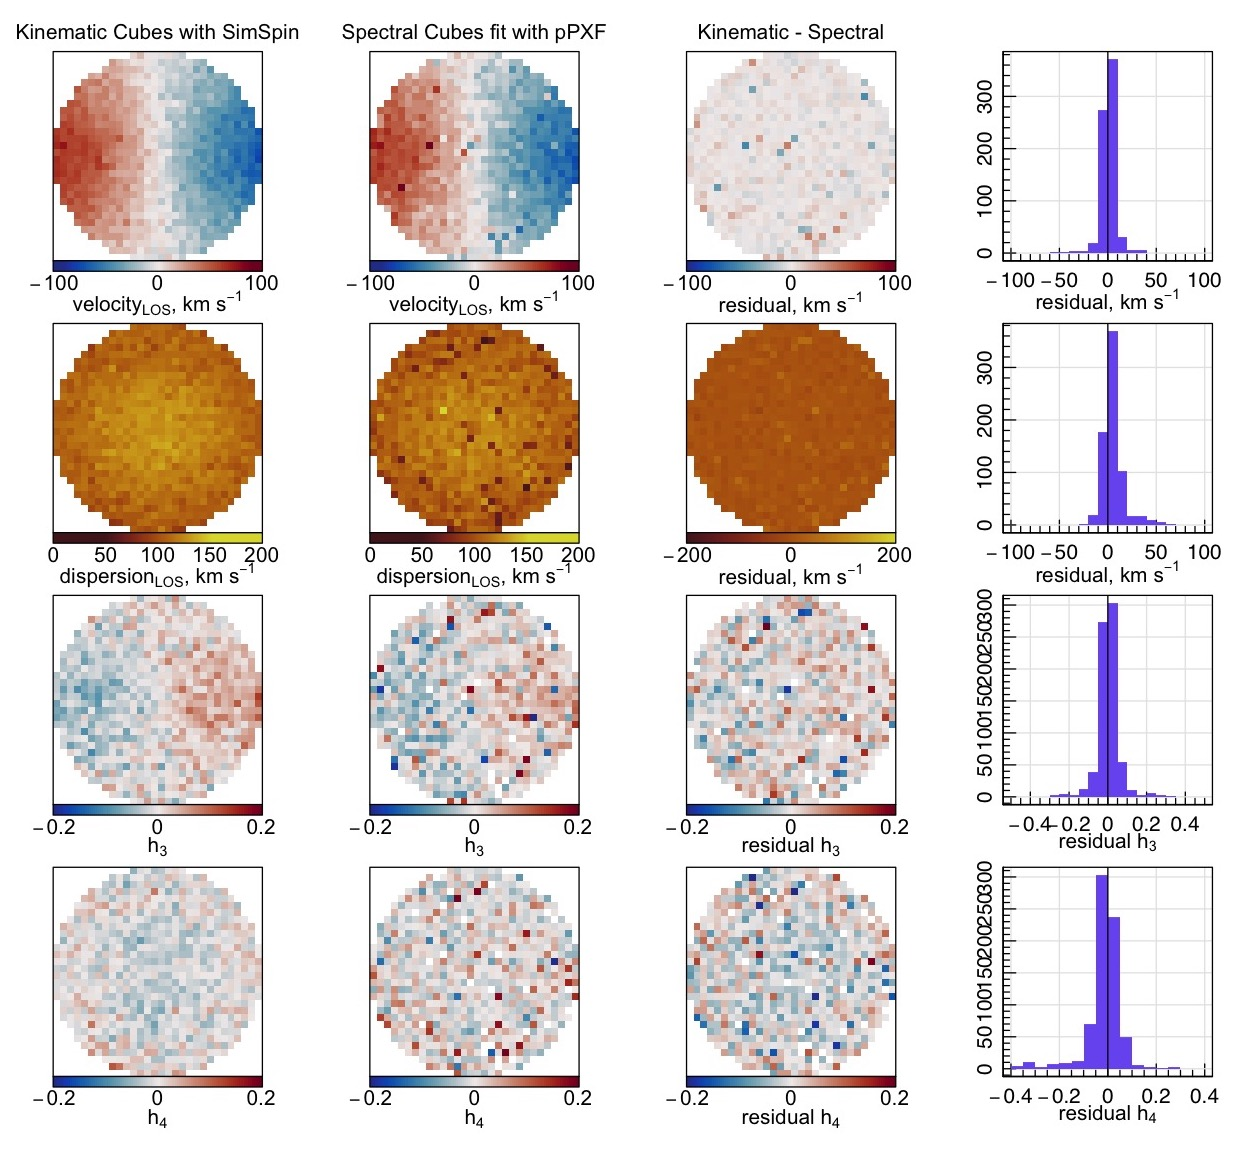
\includegraphics[keepaspectratio, width=8cm]{Figures/cs3_disk_velocities_lowz_fwhm_EMILES.jpeg}
    \caption{Case Study 3: The disk model built with EMILES templates observed with an intrinsic telescope resolution of  $\lambda_{\text{LSF}}^{telescope} = 3.61$ \AA{} at a low redshift distance of $z = 0.0144$. Here we compare the output kinematic cubes to the kinematics fit with pPXF.}
    \label{fig:cs3_disk_lowz_EMILES}
\end{figure}

\begin{figure}
    \centering
    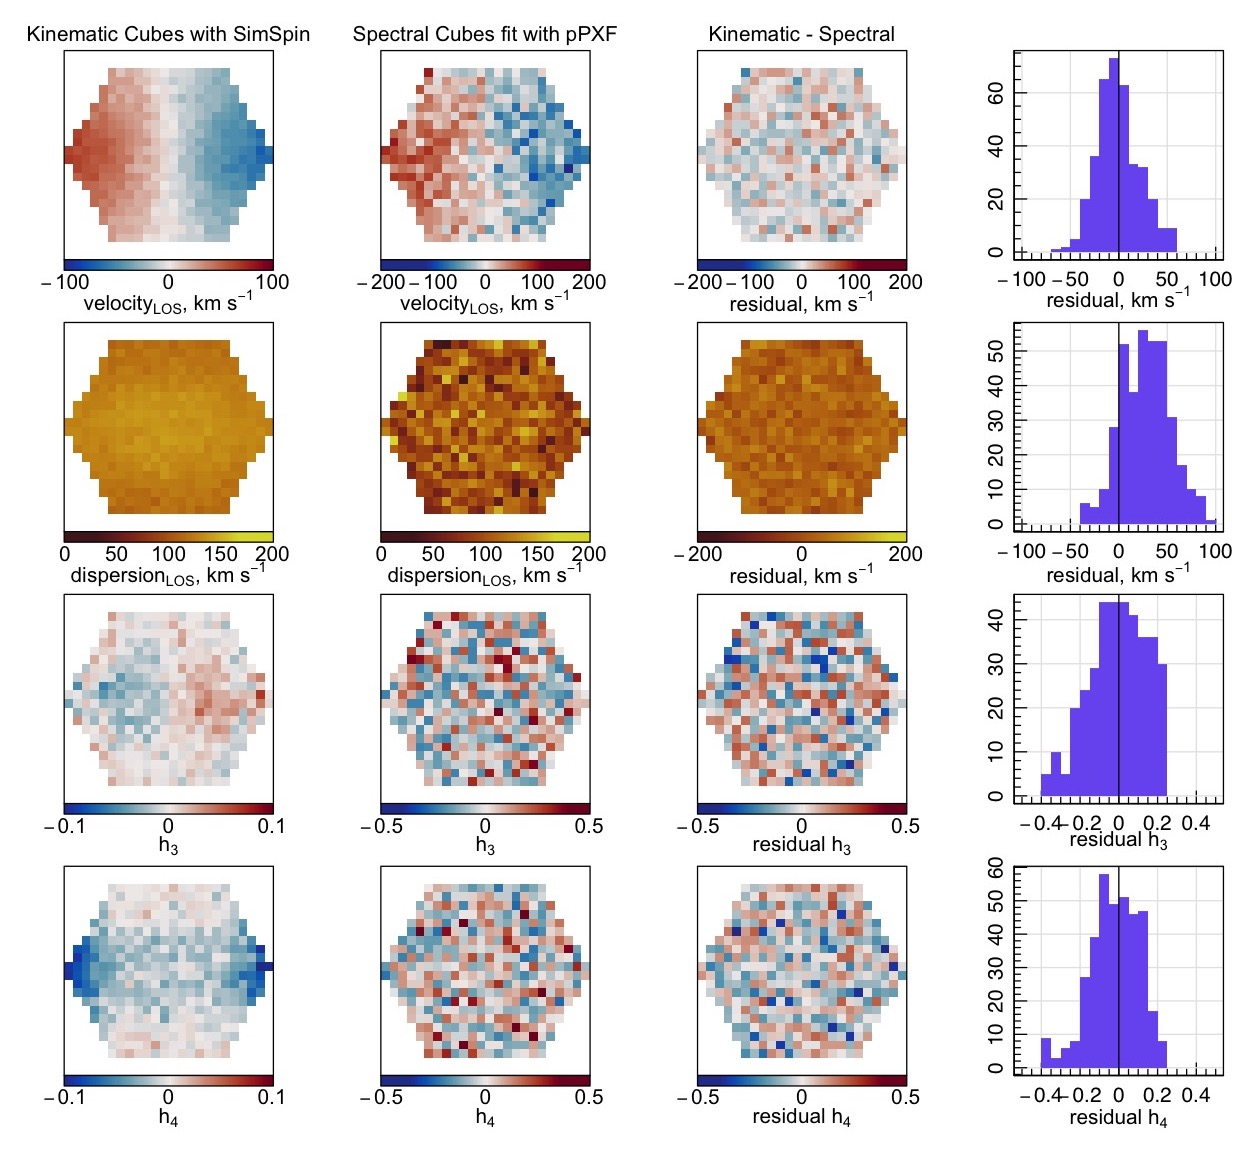
\includegraphics[keepaspectratio, width=8cm]{Figures/cs3_disk_velocities_lowz_fwhm_BC03.jpeg}
    \caption{Case Study 3: The disk model built with BC03 templates observed with an intrinsic telescope resolution of  $\lambda_{\text{LSF}}^{telescope} = 4.56$ \AA{} at a low redshift distance of $z = 0.0144$. Here we compare the output kinematic cubes to the kinematics fit with pPXF.}
    \label{fig:cs3_disk_lowz_BC03}
\end{figure}

\FloatBarrier

\subsection{Observations of with \telescope{} spectral resolution with atmospheric seeing conditions included.}
\label{app:cs4}

Here, in Figures \ref{fig:cs4_disk_highz_EMILES}-\ref{fig:cs4_disk_lowz_BC03}, we present the young disc high-$z$ observations for the EMILES model and low-$z$ observations for the BC03 model from case study 4, where we have used \telescope{} spectral resolutions of 3.61\AA{} and 4.56\AA{} for the EMILES and BC03 models respectively, and added different levels of seeing conditions by convolving each spatial plane with a convolution kernel. The hexagonal maps are those models that have been built with the BC03 templates, while the circular maps have been built with the EMILES templates. 

\begin{figure}
    \centering
    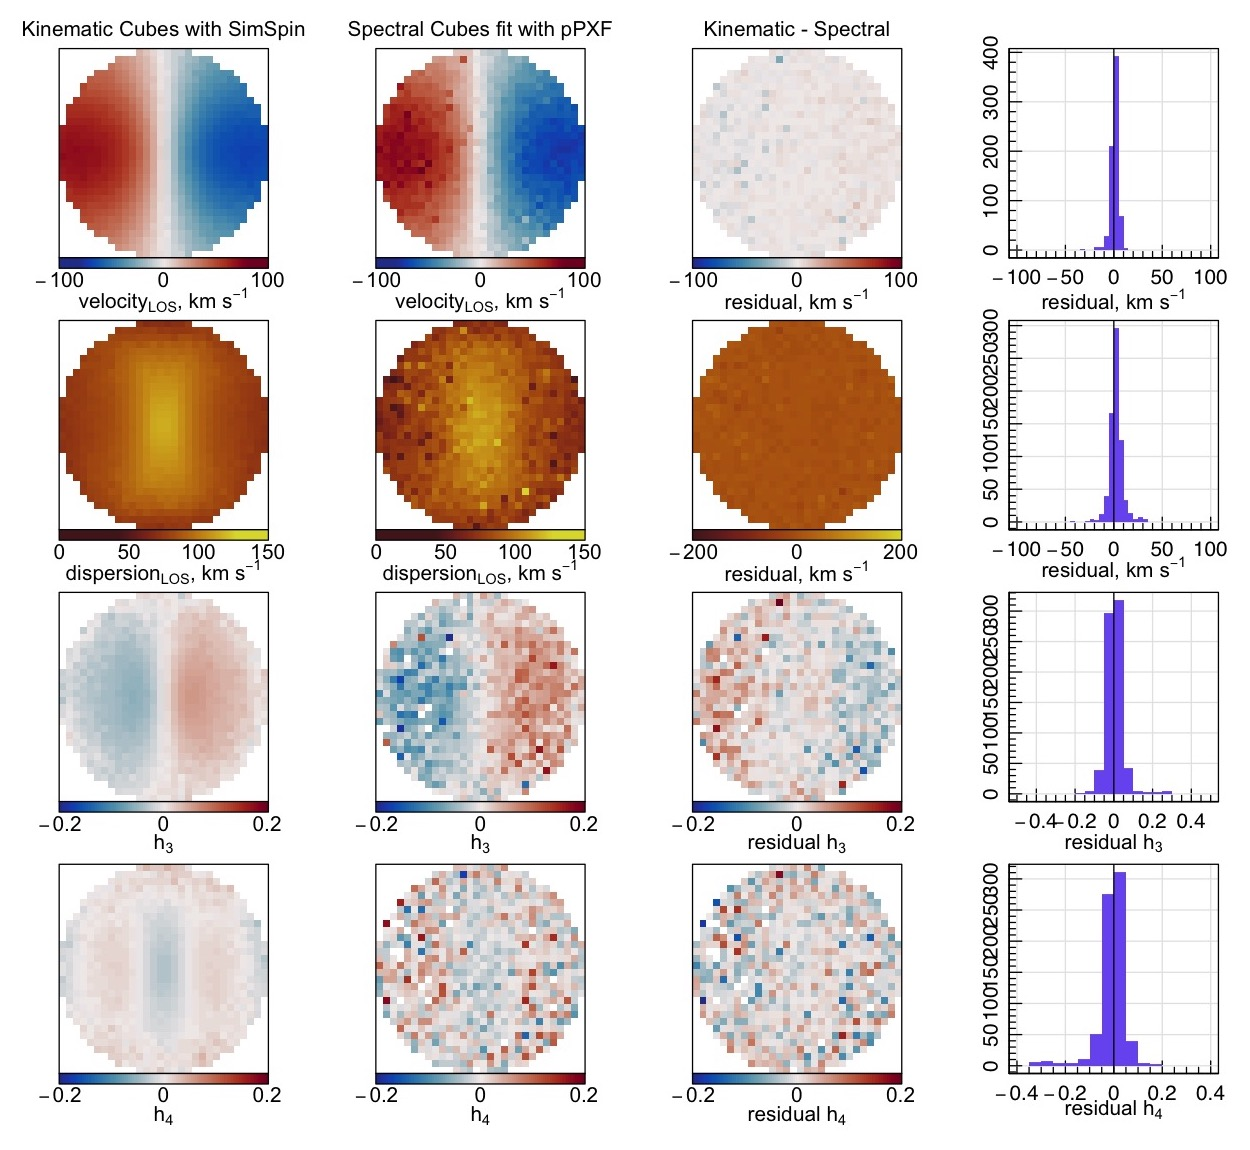
\includegraphics[keepaspectratio, width=8cm]{Figures/cs4_disk_velocities_highz_fwhm_blur_EMILES.jpeg}
    \caption{Case Study 4: The disk model built with EMILES templates observed with an intrinsic telescope resolution of  $\lambda_{\text{LSF}}^{telescope} = 3.61$ \AA{} at a high redshift distance of $z = 0.3$. We convolve each plane in this cube with a Moffat kernel with FWHM of 2.8 arcsec. Here we compare the output kinematic cubes to the kinematics fit with pPXF.}
    \label{fig:cs4_disk_highz_EMILES}
\end{figure}

\begin{figure}
    \centering
    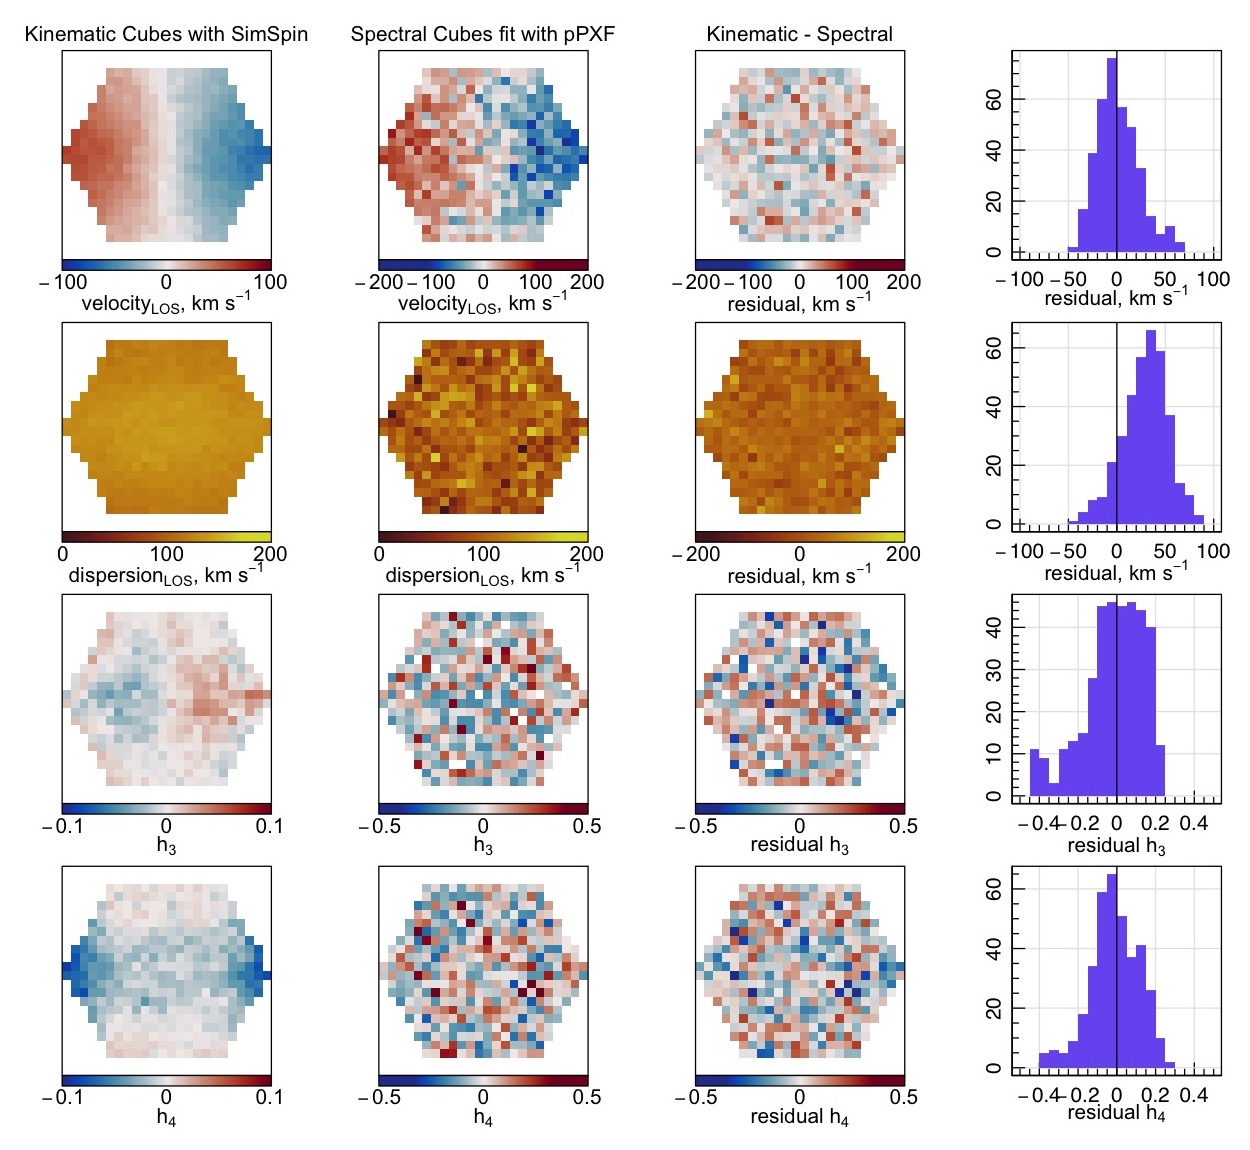
\includegraphics[keepaspectratio, width=8cm]{Figures/cs4_disk_velocities_lowz_fwhm_blur_BC03.jpeg}
    \caption{Case Study 3: The disk model built with BC03 templates observed with an intrinsic telescope resolution of  $\lambda_{\text{LSF}}^{telescope} = 4.56$ \AA{} at a low redshift distance of $z = 0.0144$. We convolve each plane in this cube with a Gaussian kernel with FWHM of 1 arcsec. Here we compare the output kinematic cubes to the kinematics fit with pPXF.}
    \label{fig:cs4_disk_lowz_BC03}
\end{figure}


\end{document}
